
\documentclass[a4paper,12pt]{report}

\usepackage[utf8]{inputenc}
\usepackage[T1]{fontenc}
\usepackage[french]{babel}
\usepackage{graphicx}
\usepackage{geometry}
\usepackage{fancyhdr}
\usepackage{tikz}
\usepackage{lmodern}
\usepackage{setspace}
\usepackage{ragged2e}
\usepackage{tocloft}
\usepackage{caption}
\usepackage{subcaption}
\usepackage{float}
\usepackage[version=4]{mhchem}
\usepackage{tabularx}
\usepackage{array}
\usepackage{amsmath}
\usepackage{amssymb}
\usepackage{xparse}

\graphicspath{{images/}}


\geometry{top=2.5cm, bottom=2.5cm, left=2.5cm, right=2.5cm}
\captionsetup[figure]{labelfont=bf, labelsep=space}
\captionsetup[table]{labelfont=bf, labelsep=space}
\setlength{\tabcolsep}{6pt}
\renewcommand{\arraystretch}{1.3}
\setlength{\cftbeforetoctitleskip}{1cm}
\setlength{\cftaftertoctitleskip}{1cm}
\renewcommand{\cfttoctitlefont}{\LARGE\bfseries\centering}
\renewcommand{\contentsname}{\centering Table des mati\`eres}
\setlength{\headheight}{60pt} % Important pour éviter les avertissements avec fancyhdr

% Environnement standard pour homogénéiser les tableaux du rapport.
\NewDocumentEnvironment{StdTable}{O{H} m m m +b}
{\begin{table}[#1]\centering\caption{#2}\label{#3}\begin{tabularx}{\textwidth}{#4}#5\end{tabularx}\end{table}}
{}

\newcommand{\chapitreencadre}[1]{
    \chapter{#1} % Numérotation activée
    \vspace*{6cm}
    \begin{center}
    \begin{tikzpicture}
        \draw[thick, rounded corners=10pt] (-1,-3) rectangle (15,3);
        \node[align=center] at (7,1.2) {\Huge \textbf{Chapitre \thechapter}};
        \node[align=center, text width=13cm] at (7,-0.8) {\Large \textbf{#1}};
    \end{tikzpicture}
    \end{center}
    \vfill
}
%hadchi ghanzido ana yasmine hhh 
\usepackage{adjustbox}
\usetikzlibrary{positioning,shapes.geometric,fit,backgrounds,calc,arrows}
\definecolor{mainblue}{RGB}{12,55,110}
\tikzset{
  seqpart/.style={draw=mainblue, fill=mainblue!12, rounded corners=3pt,
                  align=center, font=\small\sffamily,
                  minimum width=3.2cm, minimum height=0.72cm},
  seqmsg/.style={->, >=stealth, draw=mainblue!80, thick},
  seqret/.style={->, >=stealth, draw=mainblue!50, thick, dashed},
  seqlbl/.style={font=\tiny\sffamily, fill=white, inner sep=1.5pt, align=center},
  seqlife/.style={dashed, draw=gray!40},
  seqfrag/.style={draw=mainblue!50, thin, rounded corners=2pt},
  hw/.style={fill=mainblue!20, draw=mainblue!70, thin},
}
\newcommand{\actbar}[3]{\draw[hw] (#1-0.28,#2) rectangle (#1+0.28,#3);}
\newcommand{\seqA}[4]{\draw[seqmsg] (#1,#3) -- node[above,seqlbl]{#4} (#2,#3);}
\newcommand{\seqR}[4]{\draw[seqret] (#1,#3) -- node[above,seqlbl]{#4} (#2,#3);}
\newcommand{\seqF}[6]{%
  \draw[seqfrag] (#1,#2) rectangle (#3,#4);
  \node[font=\tiny\sffamily\bfseries,text=mainblue] at (#1+0.9,#2-0.18){#5};
  \node[font=\tiny\sffamily,text=mainblue!75,align=center]
        at ({(#1+#3)/2},#2-0.38){#6};}
\newcommand{\CPA}{0}
\newcommand{\CPB}{5.5}
\newcommand{\CPC}{12}
\newcommand{\CPD}{18.5}
\newcommand{\CPE}{25}

%sala hadakchi lli zedt ana yasmine 

% ------------------ DÉBUT DU DOCUMENT ------------------
\begin{document}

% ------------------ PAGE DE GARDE ------------------
\pagenumbering{gobble} % Pas de numéro
\begin{center}
\begin{minipage}{0.25\textwidth}
    
\includegraphics[width=2.5cm]{logo fsbm.png}
\end{minipage}
\begin{minipage}{0.45\textwidth}
    \centering
    {\large \textbf{UNIVERSITÉ HASSAN II}}\\[0.1cm]
    {\normalsize Faculté des Sciences Ben M'Sick}
\end{minipage}
\begin{minipage}{0.25\textwidth}
    \flushright
    
\includegraphics[width=3.5cm]{logo dep.png}
\end{minipage}
\end{center}

\vspace{1.5cm}

\begin{center}
    {\normalsize \textit{Filière : Licence Fondamentale -- Développement Informatique }}\\[0.8cm]

    \textsc{\large Mémoire de fin d'étude }\\[0.8cm]
    \rule{\linewidth}{0.4pt}\\[0.4cm]
    {\Huge \textbf{Conception et Développement d'une Plateforme Web Touristique Unifiée  }}\\[0.4cm]
    \rule{\linewidth}{0.4pt}\\[1.5cm]

 \begin{minipage}{\textwidth}

        \textbf{Réalisé par :}\\
        EL AATIFI Sara\\
        KBABRA Yasmine
    \end{minipage}

    \hfill
    \begin{minipage}{0.45\textwidth}
        \raggedleft
        \textbf{Encadré par  :}\\
        Pr. Soumaya OUNACER (Encadrante)  \\ Mme F. ABBOUR (Co-encadrante) 
    \end{minipage}
\vspace{1.5cm}

\begin{minipage}{\textwidth}
\begin{flushleft}
\textbf{Soutenu le 13 Juin 2026 devant le jury composé de :}\\[0.2cm]
\vspace{0.5cm}
\begin{tabular}{l l}
Pr.       \\
Pr.  \\
Pr.  \\
\end{tabular}
\end{flushleft}
\end{minipage}
\end{center}

\begin{center}

\vspace{2cm}

    {\large Année Universitaire 2025--2026}

    \end{center}



% ------------------ EN-TÊTE ------------------
\newpage
\pagenumbering{arabic}
\pagestyle{fancy}
\fancyhf{}
\fancyhead[L]{\raisebox{-10pt}{
\includegraphics[height=1.5cm]{logo fsbm.png}}}
\fancyhead[R]{\raisebox{-10pt}{
\includegraphics[height=1.5cm]{logo dep.png}}}

\fancyfoot[C]{\thepage}

% ------------------ DÉDICACE ------------------
\newpage
\vspace*{\fill}
\begin{flushright}
    \Huge \textit{À nos très chers parents\ldots}
\end{flushright}
\vspace*{\fill}

% ------------------ REMERCIEMENTS ------------------
\newpage
\vspace*{0.5cm}
\begin{center}
    {\LARGE\textbf{\textit{REMERCIEMENTS}}}
\end{center}
\vspace{2cm}

\justifying{   Ce mémoire est bien plus qu’un travail académique : il incarne le reflet d’un chemin parcouru à deux, marqué par la rigueur, la persévérance, les remises en question. . . et une solidarité constante.
\vspace*{0.5cm}

  Nous tenons à adresser nos plus sincères remerciements à notre encadrante, Pr. \textbf{OUNACER Soumaya}, pour la confiance qu’elle nous a accordée, son accompagnement précieux, sa disponibilité ainsi que la richesse de ses conseils tout au long de notre parcours universitaire et particulièrement durant la réalisation de ce mémoire de fin d’études. Son encadrement rigoureux, ses orientations pertinentes et son soutien constant ont constitué un apport essentiel à l’aboutissement de ce travail. Nous exprimons également notre profonde gratitude à Mme \textbf{ABBOUR FATIMA ZAHRA} pour son accompagnement, sa disponibilité et les précieux conseils apportés durant la période d’encadrement de notre projet de fin d’études. Son soutien et ses orientations nous ont permis de mener ce travail dans les meilleures conditions.
\vspace*{0.5cm}

Nous remercions également l’ensemble du corps enseignant de la \textbf{Faculté des Sciences Ben M'Sick}, pour la richesse de leurs enseignements, leur accompagnement et leur implication tout au long de notre formation.
\vspace*{0.5cm}

Travailler en binôme a été une véritable force. Nous avons partagé les efforts, les idées, les doutes et les réussites, mais aussi les rires et les longues heures de réflexion. Cette aventure commune nous a permis de mieux nous découvrir, de nous compléter et de nous soutenir mutuellement. C’est ensemble que nous sommes fières du chemin parcouru.
\vspace*{0.5cm}

Nous adressons également nos sincères remerciements à nos familles respectives, pour leur soutien indéfectible, leur confiance et leur patience. Merci à nos parents, qui ont toujours su que nous pouvions y arriver, même lorsque nous doutions.
Enfin, merci à cette petite voix en nous qui nous rappelle chaque jour que rêver, c’est bien … mais persévérer, c’est mieux.
}

 
\vspace{0.5cm}
\begin{spacing}{1.5}
\justifying


\end{spacing}

% ------------------ RESUME ------------------
\newpage
\vspace*{0.5cm}
\begin{center}
    {\LARGE\textbf{\textit{RÉSUMÉ }}}
\end{center}
%Ce rapport présente le travail réalisé dans le cadre du Projet de Fin d’Études de la Licence Fondamentale en Développement Informatique à la Faculté des Sciences Ben M’Sick de l’Université Hassan II de Casablanca. Le projet consiste en la conception et le développement de \textbf{TravEasy}, une plateforme web touristique unifiée destinée à centraliser les principaux services liés au tourisme au Maroc. Elle permet aux utilisateurs de découvrir des destinations touristiques, de bénéficier de recommandations d’hôtels adaptées à leurs besoins, de réserver des moyens de transport vers et depuis les aéroports, ainsi que de consulter et partager des avis au sein d’un espace communautaire. Dotée d’une interface bilingue français–anglais, la plateforme vise à offrir une expérience fluide, sécurisée et accessible à une clientèle nationale et internationale, tout en contribuant à la valorisation du tourisme marocain à travers les technologies numériques.
Ce rapport présente le travail réalisé dans le cadre du Projet de Fin d'Études de la Licence Fondamentale en Développement Informatique à la Faculté des Sciences Ben M'Sick de l'Université Hassan II de Casablanca.
Ce projet porte sur la conception et le développement de TravEasy, une plateforme web touristique unifiée ayant pour objectif de centraliser et de simplifier l'accès aux principaux services liés au tourisme au Maroc.La plateforme permet aux utilisateurs de découvrir des destinations et sites touristiques, d'accéder à des informations détaillées et actualisées sur les lieux d'intérêt, de rechercher des hébergements adaptés à leurs préférences et à leur budget grâce à un système de filtrage, ainsi que d'effectuer des réservations d'hébergement directement au sein de la plateforme de manière simple et sécurisée. Elle offre également la possibilité de rechercher et de réserver différents moyens de transport, notamment les transferts vers et depuis les aéroports, tout en fournissant une estimation préalable des coûts de transport afin d'assurer une plus grande transparence des tarifs et d'aider les voyageurs à mieux planifier leur budget. En complément, la plateforme intègre un espace communautaire permettant aux utilisateurs de consulter, partager et échanger des avis, recommandations et expériences de voyage, favorisant ainsi une interaction enrichissante entre les membres de la communauté. Dotée d'une interface bilingue français–anglais, d'une architecture moderne et de fonctionnalités adaptées aux besoins des voyageurs nationaux et internationaux, TravEasy vise à offrir une expérience utilisateur fluide, intuitive, sécurisée et accessible, tout en contribuant à la promotion du patrimoine touristique marocain et à la modernisation du secteur du tourisme grâce à l'exploitation des technologies numériques
\vspace{2cm}
\textbf{Mots-clés :} Espace communautaire, estimation des coûts, filtrage d'hébergements, Maroc, plateforme web touristique, réservation d'hébergement, réservation de transport, tourisme numérique

% ------------------ ABSTRACT ------------------
\newpage
\vspace*{0.5cm}
\begin{center}
    {\LARGE\textbf{\textit{ABSTRACT}}}
\end{center}
\vspace{2cm}




%This report presents the work carried out as part of the Final Year Project for the Bachelor’s degree in Computer Science Development at the Faculty of Sciences Ben M’Sick, Hassan II University of Casablanca. The project focuses on the design and development of \textbf{TravEasy}, a unified web-based tourism platform tailored to the Moroccan market. In response to the fragmentation of online tourism services, TravEasy provides a centralized and seamless experience that enables users to discover tourist destinations, access hotel recommendations, book airport transfers, and share reviews and ratings through a single interface. The platform also features a fully bilingual French–English interface designed to meet the needs of both local and international travelers. This project demonstrates the successful development of a complete digital solution that combines usability, performance, and security while contributing to the promotion and modernization of Moroccan tourism.

This report presents the work carried out as part of the Final Year Project for the Fundamental Bachelor's Degree in Computer Development at the Faculty of Sciences Ben M'Sick, Hassan II University of Casablanca. This project focuses on the design and development of TravEasy, a unified tourist web platform aimed at centralizing and simplifying access to the main tourism-related services in Morocco.
The platform allows users to discover destinations and tourist sites, access detailed and up-to-date information on points of interest, search for accommodations suited to their preferences and budget through a filtering system, and make hotel reservations directly within the platform in a simple and secure manner. It also offers the possibility to search for and book various means of transport, including airport transfers, while providing a preliminary estimate of transport costs to ensure greater price transparency and help travelers better plan their budget. In addition, the platform integrates a community space allowing users to consult, share and exchange reviews, recommendations and travel experiences, fostering enriching interaction among community members. Featuring a bilingual French–English interface, a modern architecture and functionalities tailored to the needs of both national and international travelers, TravEasy aims to provide a smooth, intuitive, secure and accessible user experience, while contributing to the promotion of Morocco's tourist heritage and the modernization of the tourism sector through the use of digital technologies


\textbf{Keywords:} Accommodation booking, community space, cost estimation, digital tourism, accommodation filtering, Moroccan tourism, tourist web platform, transport booking

% ------------------ TABLE DES MATIÈRES ------------------
\newpage
\tableofcontents

% ------------------ LISTE DES FIGURES ------------------
\newpage
\listoffigures


% ------------------ LISTE DES TABLEAUX ------------------
\newpage
\listoftables

% ------------------ LISTE DES ABRÉVIATIONS ------------------
\newpage
\section*{Liste des abréviations}
\addcontentsline{toc}{section}{Liste des abréviations}

\vspace{0.5cm}

\begin{spacing}{1.3}

\begin{tabular}{p{3cm} p{11cm}}

\textbf{API} & Application Programming Interface \\

\textbf{SSO} & Single Sign-On \\

\textbf{REST} & Representational State Transfer \\

\textbf{UI} & User Interface \\

\textbf{UX} & User Experience \\

\textbf{UML} & Unified Modeling Language \\

\textbf{SQL} & Structured Query Language \\

\textbf{JSON} & JavaScript Object Notation \\

\textbf{PDF} & Portable Document Format \\

\textbf{HTTP} & HyperText Transfer Protocol \\

\textbf{HTTPS} & HyperText Transfer Protocol Secure \\

\textbf{2FA} & Two-Factor Authentication \\

\textbf{TLS} & Transport Layer Security \\

\textbf{VTC} & Véhicule de Tourisme avec Chauffeur \\

\textbf{ERD} & Entity Relationship Diagram \\

\textbf{PCI-DSS} & Payment Card Industry Data Security Standard \\

\textbf{CMI} & Centre Monétique Interbancaire \\

\textbf{SMS} & Short Message Service \\

\textbf{OWASP} & Open Web Application Security Project \\

\textbf{VPS} & Virtual Private Server \\

\textbf{CI/CD} & Continuous Integration / Continuous Deployment \\

\textbf{SMTP} & Simple Mail Transfer Protocol \\

\end{tabular}

\end{spacing}


% ------------------ INTRODUCTION ------------------
\newpage
\section*{Introduction Générale}
\addcontentsline{toc}{section}{Introduction}
\vspace{0.5cm}
\begin{spacing}{1.5}
\justifying

Le secteur du \textbf{tourisme} constitue un levier important du développement économique du Maroc, contribuant à la croissance, à la création d’emplois et au rayonnement du pays à l’échelle internationale. Avec l’essor des technologies numériques et l’évolution des attentes des voyageurs, les besoins se tournent de plus en plus vers des services accessibles, centralisés et adaptés à une expérience utilisateur simplifiée.
\vspace{0.5cm}


Dans ce contexte, la digitalisation des services touristiques apparaît comme un enjeu majeur. Cependant, malgré la richesse de l’offre touristique marocaine, les solutions existantes demeurent souvent fragmentées, rendant l’organisation des séjours plus complexe et moins fluide pour les utilisateurs.
\vspace{0.5cm}

C’est dans cette optique qu’a été développé \textbf{TravEasy}, une plateforme web touristique conçue pour centraliser différents services liés au tourisme au Maroc à travers une interface unique. La plateforme propose des informations sur les destinations touristiques, un module d’hébergement permettant la consultation et la recherche d’hôtels, de riads, d’auberges et de maisons d’hôtes, des fonctionnalités de réservation de transport depuis et vers les aéroports, ainsi qu’un espace dédié aux activités touristiques et à l’interaction des utilisateurs à travers un système d’avis et de notation. Une interface bilingue français/anglais a également été intégrée afin de répondre aux besoins d’une clientèle locale et internationale.
\vspace{0.5cm} 

Ce projet s’inscrit ainsi dans une démarche de conception d’une solution numérique moderne, intuitive et performante, visant à améliorer l’expérience utilisateur tout en contribuant à la valorisation de l’offre touristique marocaine.
\vspace{0.5cm} 
Le présent rapport est structuré en cinq chapitres principaux. Le premier chapitre présente l’organisme d’accueil ainsi que le cadre académique dans lequel s’inscrit ce projet. Le deuxième chapitre est consacré à l’étude préalable et à l’analyse des besoins ; il expose la problématique, les objectifs du projet, l’étude de l’existant ainsi que les besoins fonctionnels et non fonctionnels de la plateforme. Le troisième chapitre porte sur la conception du système et présente l’architecture de la solution ainsi que les différents diagrammes UML élaborés pour modéliser les fonctionnalités du système. Le quatrième chapitre décrit la phase de réalisation et d’implémentation en détaillant les technologies utilisées, l’environnement de développement et les différents modules développés au sein de la plateforme. Le cinquième chapitre est dédié aux tests et à la validation de la solution, en présentant les différentes stratégies de test adoptées ainsi que les résultats obtenus. Enfin, le rapport se clôture par une conclusion générale qui résume les principaux résultats du projet et présente les perspectives d’amélioration et d’évolution de la plateforme TravEasy.
\end{spacing}

% ------------------ PRÉSENTATION DE L'ORGANISME ------------------
\chapter{ Présentation de l'organisme}


%yasmine
\section{Introduction}
\vspace{0.5cm}
\begin{spacing}{1.5}
\justifying
Dans le cadre de notre formation en \textbf{Développement Informatique} à la \textbf{Faculté des Sciences Ben M’Sick}, il est essentiel de réaliser un projet de fin d’études permettant de mettre en pratique les connaissances théoriques et techniques acquises durant le cursus universitaire. Ce chapitre a pour objectif de présenter l’établissement d’accueil de la formation, à savoir la Faculté des Sciences Ben M’Sick, ainsi que le \textbf{Département Mathématiques et Informatique} et la filière \textbf{Développement Informatique}. Il introduit également le contexte général du projet réalisé, portant sur la conception et le développement d’une plateforme web touristique unifiée destinée à centraliser différents services touristiques et à améliorer l’expérience des utilisateurs.

\end{spacing}
\section{Présentation de la Faculté des Sciences Ben M’Sick}
\vspace{0.5cm}
\begin{spacing}{1.5}
\justifying
Faculté des Sciences Ben M'Sick est un établissement relevant de l’\textbf{Université Hassan II de Casablanca}. Elle assure la formation des étudiants dans plusieurs domaines scientifiques et technologiques tout en favorisant la recherche scientifique et l’innovation.

\begin{figure}[H]
    \centering
    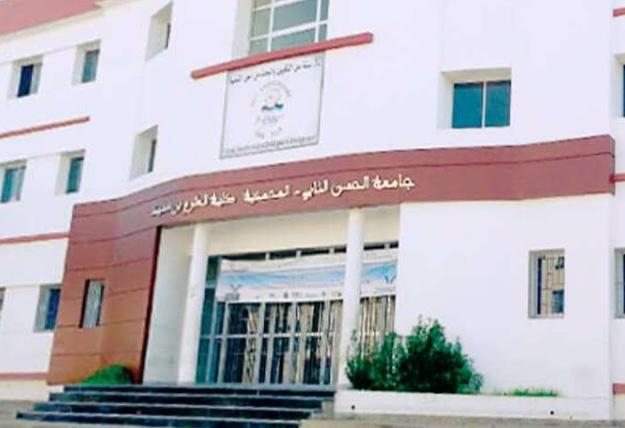
\includegraphics[width=0.7\textwidth]{img_fac.png}
    \caption{Image de la Faculté des Sciences Ben M’Sick }
    \label{fig:faculté_sciences_ben_m_sick}
\end{figure}
\end{spacing}
\section{Présentation du Département Mathématiques et Informatique}
\vspace{0.5cm}
\begin{spacing}{1.5}
\justifying
Le \textbf{Département Mathématiques et Informatique} est chargé de l’encadrement pédagogique et scientifique des formations liées aux mathématiques et à l’informatique. Il vise à développer les compétences techniques et méthodologiques des étudiants à travers des enseignements théoriques et pratiques dans différents domaines de l’informatique.

Le département encourage également la réalisation de projets académiques permettant aux étudiants de renforcer leurs compétences en développement et en gestion des systèmes informatiques.
\end{spacing}
\section{Présentation de la Filière Développement Informatique}
\vspace{0.5cm}
\begin{spacing}{1.5}
\justifying
La filière \textbf{Développement Informatique} a pour mission de former des étudiants capables de concevoir, développer et maintenir des applications informatiques répondant aux besoins des organisations et des utilisateurs. Elle offre une formation alliant connaissances théoriques et compétences pratiques dans les domaines du développement logiciel, des bases de données, des systèmes d’information, des technologies web et de l’ingénierie logicielle.

Grâce à un programme pédagogique diversifié, la filière permet aux étudiants d’acquérir les compétences techniques et méthodologiques nécessaires à la réalisation de projets informatiques, tout en développant leur capacité d’analyse, de résolution de problèmes et d’adaptation aux évolutions technologiques. Elle prépare ainsi les futurs diplômés à intégrer le monde professionnel ou à poursuivre leurs études dans des domaines spécialisés de l’informatique.

\end{spacing}

\section{Conclusion}
\vspace{0.5cm}
\begin{spacing}{1.5}
\justifying
%yasmine
À travers ce chapitre, nous avons présenté le cadre académique dans lequel s’inscrit ce projet de fin d’études, en mettant en lumière la Faculté des Sciences Ben M’Sick, le Département Mathématiques et Informatique ainsi que la filière Développement Informatique. Ces structures offrent un environnement propice à l’acquisition de compétences théoriques et pratiques dans le domaine du développement logiciel. Le projet réalisé, portant sur la conception et le développement de la plateforme web touristique unifiée \textbf{TravEasy}, constitue une application concrète des connaissances acquises au cours de la formation. Le chapitre suivant sera consacré à l’étude du contexte du projet, à l’analyse des besoins ainsi qu’à la définition des principales fonctionnalités de la plateforme.

\end{spacing}
\newpage
\begin{spacing}{0.5}
\chapter{ Étude préalable et analyse des besoins}
\end{spacing}

\newpage
\section{Introduction}
\vspace{0.5cm}
\begin{spacing}{1.5}
\justifying
Dans un contexte de transformation numérique du secteur touristique, les voyageurs recherchent aujourd’hui des solutions digitales capables de centraliser les différents services liés à leurs déplacements. Malgré l’existence de nombreuses plateformes de réservation et de planification touristique, la plupart restent limitées à des fonctionnalités spécifiques, obligeant les utilisateurs à utiliser plusieurs applications pour organiser un même séjour.

C’est dans ce cadre que s’inscrit notre projet de fin d’études portant sur la conception d’une plateforme web touristique unifiée adaptée au contexte marocain. Cette solution vise à offrir une interface centralisée permettant aux utilisateurs de gérer leurs déplacements, réservations et activités touristiques de manière simple et efficace.

Ce chapitre a pour objectif de présenter le contexte général du projet, d’analyser les limites des solutions existantes et d’identifier les besoins fonctionnels et non fonctionnels nécessaires à la conception du système, tout en prenant en considération les acteurs, les contraintes et la planification du projet.
\end{spacing}

\section{Présentation du projet}
\vspace{0.5cm}
\begin{spacing}{1.5}
\justifying
Le tourisme est un secteur économique important qui connaît une forte évolution grâce à la transformation numérique. Au Maroc, ce domaine occupe une place stratégique et bénéficie du développement des services digitaux liés au voyage. Cependant, les plateformes touristiques actuelles restent souvent limitées à des services spécifiques, obligeant les utilisateurs à utiliser plusieurs applications pour organiser un même séjour.

Cette fragmentation complique l’expérience utilisateur, notamment dans le contexte marocain où certains besoins comme la transparence des coûts de transport et l’intégration des moyens de paiement locaux restent insuffisamment pris en charge. Dans ce cadre, notre projet vise la conception d’une plateforme web touristique unifiée permettant de centraliser les principaux services touristiques au sein d’une interface unique afin de simplifier l’organisation des voyages et d’améliorer l’expérience utilisateur.

\end{spacing}

\section{Problématique}
\vspace{0.5cm}
\begin{spacing}{1.5}
\justifying
Les plateformes touristiques actuelles proposent généralement des services séparés, obligeant les voyageurs à utiliser plusieurs applications pour organiser un seul voyage. Cette fragmentation complique la gestion des réservations et réduit la fluidité de l’expérience utilisateur.

Notre projet vise donc à répondre à la problématique suivante :

« Comment concevoir une plateforme web capable de centraliser les différents services touristiques dans une interface unique, sécurisée et facile à utiliser ? »

\end{spacing}

\section{Objectifs du projet}
\vspace{0.5cm}
\begin{spacing}{1.5}
\justifying
Le projet a pour objectifs de :

\begin{itemize}
    \item Centraliser plusieurs services touristiques au sein d’une seule plateforme
    \item Faciliter la recherche d'hébergements, la réservation de transports aéroportuaires et la découverte de destinations touristiques.
    \item Proposer un système de filtrage d'hébergements permettant aux voyageurs de trouver des options adaptées à leur budget et à leurs préférences
    \item Offrir un moteur de recherche avancé avec plusieurs filtres
    \item Permettre aux utilisateurs de consulter et publier des avis
    \item Garantir la sécurité des paiements et des données personnelles
    \item Fournir une plateforme multilingue adaptée aux utilisateurs internationaux
\end{itemize}

\end{spacing}

\section{Étude de l’existant}
\vspace{0.5cm}
\begin{spacing}{1.5}
\subsection{Analyse des solutions existantes}
\justifying
Avant de développer une plateforme touristique unifiée, il est essentiel d’analyser les solutions existantes afin d’identifier leurs points forts, leurs limites et les opportunités d’amélioration. Le marché du tourisme en ligne est aujourd’hui dominé par plusieurs plateformes spécialisées qui couvrent chacune un segment précis du parcours voyageur (hébergement, transport, activités ou avis), mais sans offrir une véritable intégration globale.

Dans le cadre de cette étude, une analyse comparative a été réalisée sur plusieurs acteurs majeurs du secteur, notamment \textbf{Google Travel, Booking.com, Airbnb, TripAdvisor, Expedia, GetYourGuide et Uber}. L’objectif est d’évaluer leurs fonctionnalités, leur niveau d’intégration, leur couverture du marché marocain ainsi que leur capacité à répondre aux besoins des utilisateurs.


\begin{StdTable}[h]{Comparatif des plateformes touristiques existantes}{tab:comparatif}{|X|X|X|X|X|X|X|X|}
    \hline
    Plateforme & Hébergement & Transport aéroport & Lieux touristiques & Avis utilisateurs & Multilingue FR/EN & Paiement local Maroc & Transparence prix \\
    \hline
    Google Travel & Oui (agrégation) & Non & Oui (agrégation) & Oui & Partiel & Non & Variable \\
    \hline
    Booking.com & Très étendu & Partiel & Non & Très étendu & Oui & Non & Faible \\
    \hline
    Airbnb & Oui (particuliers) & Non & Partiel & Oui & Oui & Non & Sans objet \\
    \hline
    Tripadvisor & Agrégation & Non & Oui & Très étendu & Oui & Non & Sans objet \\
    \hline
    Expedia & Très étendu & Partiel & Activités & Moyen & Oui & Non & Moyenne \\
    \hline
    GetYour Guide & Absent & Non & Activités seules & Oui & Oui & Non & Sans objet \\
    \hline
    Uber & Non & Oui & Non & Partiel & Partiel & Non & Sans objet \\
    \hline
    \end{StdTable}

Cette analyse montre qu’aucune plateforme ne propose une centralisation complète du parcours touristique. Chacune reste spécialisée dans un domaine précis, ce qui limite la continuité et la fluidité de l’expérience utilisateur.

% Une seconde analyse plus approfondie a été menée en intégrant des critères liés à l’expérience utilisateur, tels que les avis, le multilinguisme, les paiements locaux et la transparence des prix.


% \begin{StdTable}[h]{Comparatif des plateformes}{tab:comparatif_plateformes_2}{|X|X|X|X|X|X|}
% \hline
% Plateforme    & Hébergement & Avis \newline utilisateurs & Multilingue & Paiement local Maroc & Transparence prix \newline transport \\
% \hline
% Google \newline Travel & Oui         & Oui               & Oui         & Non                  & Variable                    \\
% \hline
% Booking.com   & Très étendu & Très étendu       & Oui         & Non                  & Faible                      \\
% \hline
% Airbnb        & Très étendu & Oui               & Oui         & Non                  & Sans objet                  \\
% \hline
% Tripadvisor   & Agrégation  & Très étendu       & Oui         & Non                  & Sans objet                  \\
% \hline
% Expedia       & Très étendu & Moyen             & Oui         & Non                  & Moyenne                     \\
% \hline
% GetYour \newline Guide  & Absent      & Oui               & Oui         & Non                  & Sans objet                  \\
% \hline
% Uber          & Absent      & Oui               & Oui         & Partiel              & Bonne                      \\
% \hline
% \end{StdTable}
% Cette seconde analyse confirme que, malgré leur maturité, ces plateformes ne répondent pas pleinement aux besoins spécifiques du marché marocain. Les principales limites concernent l’intégration des moyens de paiement locaux, la couverture des services de transport interurbain et la transparence des tarifs, notamment pour les voyageurs internationaux.

 \end{spacing}

\subsection{Synthèse critique de l’existant}
\vspace{0.5cm}
\begin{spacing}{1.5}
\justifying
L’étude comparative met en évidence plusieurs limites communes aux plateformes touristiques existantes.

Tout d’abord, aucune solution ne propose une gestion complète et centralisée du parcours touristique, obligeant les utilisateurs à utiliser plusieurs plateformes spécialisées pour organiser leur voyage. Cette fragmentation rend l’expérience moins fluide et plus complexe.

Ensuite, les plateformes actuelles prennent peu en compte les spécificités du marché marocain, notamment en matière de moyens de paiement, de couverture géographique et d’adaptation aux services locaux.

Par ailleurs, le transport aéroportuaire constitue une faiblesse notable, avec une intégration souvent partielle, une visibilité limitée des prix et une couverture inégale des zones desservies.

Enfin, la dispersion des informations touristiques oblige les voyageurs à consulter plusieurs sources pour obtenir une vision complète de leur séjour.

Ces limites confirment donc la nécessité de développer une plateforme touristique unifiée, capable de centraliser les services essentiels tout en répondant aux besoins spécifiques du contexte marocain.
\end{spacing}

\subsection{Valeur ajoutée de la solution proposée}
\vspace{0.5cm}
\begin{spacing}{1.5}
\justifying
La plateforme proposée se distingue par une approche intégrée visant à centraliser l’ensemble des services touristiques (transport, hébergement, activités, recommandations et réservation) au sein d’une seule interface, afin de simplifier le parcours utilisateur. Elle met également l’accent sur la transparence des prix, notamment pour le transport aéroportuaire, grâce à un système de calcul basé sur des critères définis (distance, type de véhicule, horaires, saison).

En outre, la solution intègre des moyens de paiement adaptés au marché marocain, renforçant ainsi son accessibilité. Enfin, elle privilégie une expérience utilisateur fluide, la sécurité des données et une conception évolutive répondant aux besoins du tourisme numérique moderne.

Contrairement à plusieurs plateformes spécialisées, TravEasy permet de centraliser la recherche et la réservation d'hébergements touristiques au Maroc au sein d'un même environnement numérique. Grâce à un système de recherche multicritère et à une interface intuitive, l'utilisateur peut comparer plusieurs établissements et effectuer sa réservation directement sur la plateforme, sans être redirigé vers un site externe
\subsection{Présentation des acteurs du système}
\vspace{0.5cm}
\begin{spacing}{1.5}
\justifying
Cette section s’inscrit dans l’analyse fonctionnelle de la plateforme web touristique unifiée et vise à identifier les principaux acteurs du système ainsi que leurs rôles et interactions. Cette identification constitue une étape essentielle pour la définition des besoins fonctionnels et la modélisation du système.

\begin{StdTable}[h]{Acteurs du système TravEasy}{tab:acteurs_systeme}{|X|X|X|}
\hline
Acteur & Description & Principales interactions avec le système \\
\hline
Visiteur & Internaute non connecté souhaitant découvrir la plateforme TravEasy. & Consultation des destinations, lieux touristiques, hébergements et transports disponibles, sans possibilité de réservation ni de publication d'avis. \\
\hline
Utilisateur & Voyageur national ou international inscrit sur la plateforme souhaitant organiser son séjour au Maroc. & Recherche et filtrage des hébergements, réservation de transport, paiement sécurisé, gestion du profil et publication d'avis. \\
\hline
Administrateur & Responsable de la gestion et du bon fonctionnement global de la plateforme. & Gestion des utilisateurs, supervision des contenus, modération des avis et suivi des paiements. \\
\hline
\end{StdTable}


En résumé, l'interaction entre ces trois acteurs assure le bon fonctionnement de TravEasy : le visiteur explore librement la plateforme, l'utilisateur accède aux services de réservation et de paiement, tandis que l'administrateur veille à la sécurité, à la qualité des contenus et à la gestion globale de la plateforme
\end{spacing}

\end{spacing}
\section{Spécification des besoins}
\vspace{0.5cm}
\begin{spacing}{1.5}
\justifying
\subsection{Introduction}
\vspace{0.5cm}
\begin{spacing}{1.5}
\justifying
Cette section définit la phase de spécification des besoins comme une étape fondamentale du projet, permettant d’identifier avec précision les attentes du système. Elle met en évidence deux catégories principales de besoins : les besoins fonctionnels, qui décrivent les services attendus, et les besoins non fonctionnels, qui concernent la qualité du système (performance, sécurité, ergonomie, etc.). Cette structuration constitue une base essentielle pour la conception et le développement de la plateforme touristique.

\end{spacing}
\subsection{Besoins fonctionnels}
\vspace{0.5cm}
\begin{spacing}{1.5}
\justifying

Les besoins fonctionnels regroupent l’ensemble des services que la plateforme doit offrir aux utilisateurs. Ils sont organisés en modules afin de structurer le système :

\begin{itemize}
    \item Gestion des utilisateurs : inscription, authentification, gestion des profils et des rôles
    \item Transport aéroportuaire : réservation de trajets, estimation des coûts, paiement et géolocalisation
    \item Module touristique : recherche et consultation d’informations sur les destinations et activités
    \item Module d'hébergement : Consultation des hôtels, riads, auberges et maisons d'hôtes, recherche par nom ou ville, et réservation directement au sein de la plateforme TravEasy
    \item Réservation : gestion des réservations d’activités et transports 
    \item Avis et notation : publication d’avis, système de notation et modération
    \item Paiement sécurisé : gestion des transactions, facturation et remboursements
    \item Multilingue : support de plusieurs langues pour améliorer l’accessibilité
 Ces modules permettent de couvrir l’ensemble du parcours utilisateur de manière centralisée et cohérente
\end{itemize}
\end{spacing}


\end{spacing}

\subsection{Besoins non fonctionnels}
\vspace{0.5cm}
\begin{spacing}{1.5}
\justifying

Afin d’assurer la qualité de la plateforme, plusieurs besoins non fonctionnels doivent
être respectés :
\begin{itemize}
    \item Une interface responsive compatible avec différents appareils 
    \item Un temps de réponse rapide 
    \item La sécurité des données et des paiements 
    \item Une architecture maintenable et évolutive 
    \item Une bonne disponibilité et fiabilité du système
\end{itemize}

\end{spacing}
\section{Planification du projet}
\vspace{0.5cm}
\begin{spacing}{1.5}
\justifying
\subsection{Introduction}
\vspace{0.5cm}
\begin{spacing}{1.5}
\justifying
La planification constitue une étape essentielle dans la gestion d’un projet informatique, car elle permet d’organiser les tâches, de définir les délais et d’assurer une bonne coordination entre les différentes phases de développement.

Dans le cadre du projet TravEasy, un planning prévisionnel a été établi afin de structurer les principales étapes du développement de la plateforme web touristique unifiée, notamment l’analyse des besoins, la conception, le prototypage des interfaces, le développement backend et frontend, l’intégration des API, les tests et le déploiement.

Le suivi du projet s’est également appuyé sur une comparaison entre le planning prévisionnel et le déroulement réel des travaux, permettant d’identifier les écarts observés et de proposer des actions correctives pour améliorer la gestion du temps et l’organisation du projet.

\end{spacing}
\end{spacing}
\subsection{Déroulement des étapes du projet}
\vspace{0.5cm}
\begin{spacing}{1.5}
\justifying




Le développement du projet s’est déroulé selon plusieurs phases successives, permettant d’assurer une progression structurée et cohérente du système.

Phase 1 : Analyse et cahier des charges

Cette étape a consisté à identifier les besoins fonctionnels et non fonctionnels du système, analyser les solutions existantes et définir les objectifs du projet. Elle a permis de formaliser le cahier des charges et de déterminer les principales fonctionnalités attendues.

Phase 2 : Conception

La phase de conception a porté sur la modélisation du système, incluant l’architecture logicielle, les diagrammes UML (cas d’utilisation, classes, séquences et activités) ainsi que la structuration de la base de données.

Phase 3 : Prototypage UI/UX

Cette étape a permis de concevoir les maquettes de l’interface utilisateur afin d’améliorer l’expérience utilisateur et de définir l’organisation visuelle des différentes pages de la plateforme.

Phase 4 : Développement Backend

Le backend a été développé afin d’implémenter la logique métier de l’application, la gestion des utilisateurs, les réservations, les paiements, les avis et les échanges avec la base de données via les API REST.

Phase 5 : Développement Frontend

Le frontend a consisté en l’implémentation des interfaces graphiques interactives permettant aux utilisateurs d’interagir avec la plateforme.

Phase 6 : Intégration des API externes

Cette phase a permis l’intégration de services externes, notamment les APIs de paiement, de cartographie et de géolocalisation afin d’enrichir les fonctionnalités de la plateforme.

Phase 7 : Tests et validation

Les différents modules développés ont été testés afin de vérifier leur conformité aux besoins exprimés, leur sécurité et leurs performances.

Phase 8 : Déploiement

Enfin, le système a été mis en production et configuré afin de garantir son accessibilité et son bon fonctionnement.
\end{spacing}
\subsection{Planning prévisionnel du projet}
\vspace{0.5cm}
\begin{spacing}{1.5}
\justifying
Le planning prévisionnel du projet a été élaboré sous forme d’un diagramme de Gantt afin de répartir les tâches dans le temps et d’assurer un suivi rigoureux de l’avancement du projet.

\begin{figure}[H]
    \centering
    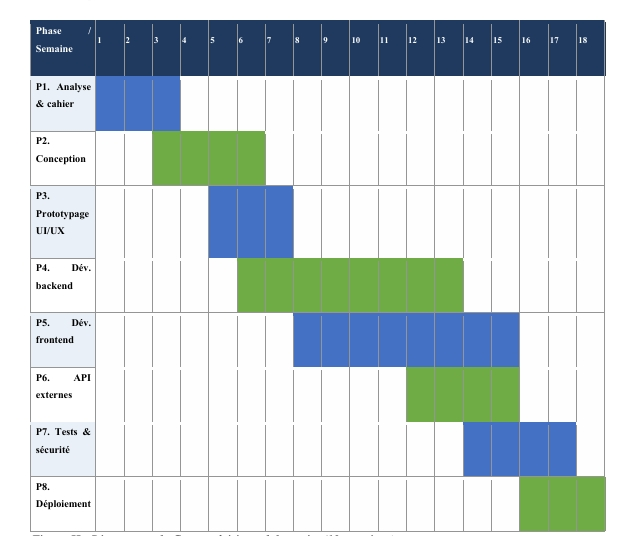
\includegraphics[width=0.50\textwidth]{di_previ.jpeg}
    \caption{ Diagramme de Gantt prévisionnel du projet}
    \label{fig: Diagramme de Gantt prévisionnel du projet }
\end{figure}

\end{spacing}
\section{Analyse des écarts entre le planning prévisionnel et réel}
\vspace{0.5cm}
\begin{spacing}{1.5}
\justifying

\subsection{Introduction}
\vspace{0.5cm}
\begin{spacing}{1.5}
\justifying
Bien qu’un planning prévisionnel ait été défini au démarrage du projet, certaines adaptations ont été nécessaires au cours du développement réel. La réalisation effective du projet s’est étalée sur une période d’environ deux mois et demi, soit environ 10 semaines, ce qui a conduit à des ajustements dans l’enchaînement et la durée des différentes activités.

\end{spacing}

\subsection{Planning réel du projet}
\vspace{0.5cm}
\begin{spacing}{1.5}
\justifying
Le diagramme suivant présente le déroulement réel du projet ainsi que la répartition effective des tâches réalisées.

\end{spacing}

\begin{figure}[H]
    \centering
    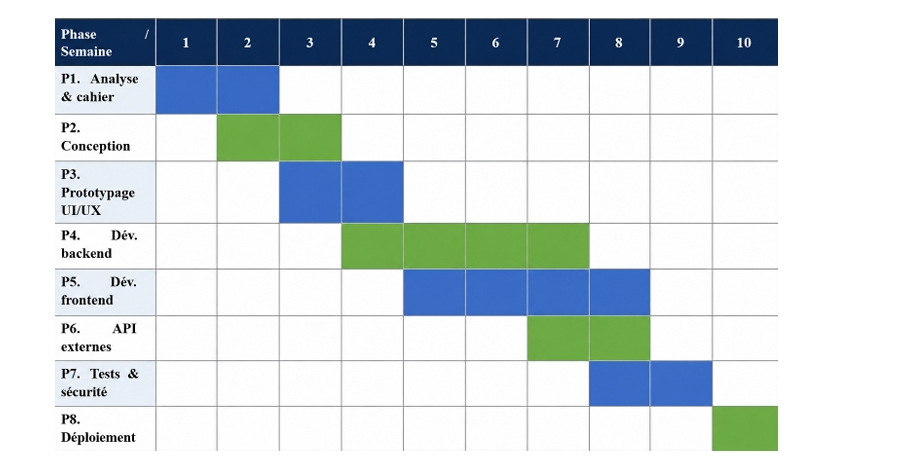
\includegraphics[width=0.50\textwidth]{di_reel.jpeg}
    \caption{Diagramme de Gantt réel du projet }
    \label{fig:Diagramme de Gantt réel du projet }
\end{figure}
\end{spacing}
\subsection{Analyse des écarts observés}
\vspace{0.5cm}
\begin{spacing}{1.5}
\justifying
L’analyse comparative entre le planning prévisionnel et le planning réel met en évidence plusieurs écarts liés à la dynamique du développement du projet.

\begin{itemize}
    \item Certaines tâches ont été réalisées plus rapidement que prévu grâce à l’utilisation de frameworks modernes facilitant le développement.
    \item Plusieurs phases ont été exécutées simultanément, notamment le développement frontend et backend, permettant un gain de temps significatif.
    \item L’intégration des APIs externes et les tests ont nécessité davantage d’ajustements techniques, entraînant quelques retours correctifs.
    \item Certaines étapes de conception ont été revues pendant le développement afin d’améliorer l’ergonomie et l’expérience utilisateur.
    \item Le projet a finalement été réalisé sur une durée plus courte que celle prévue initialement grâce à une meilleure priorisation des tâches et une organisation progressive du travail.
\end{itemize}
\end{spacing}

\subsection{Solutions proposées pour limiter les écarts}
\vspace{0.5cm}
\begin{spacing}{1.5}
\justifying
Afin de réduire les écarts entre la planification théorique et l’exécution réelle dans de futurs projets similaires, plusieurs recommandations peuvent être proposées :

\begin{itemize}
    \item Mettre en place un suivi hebdomadaire de l’avancement du projet ;
    \item Découper les tâches en sous-objectifs plus précis afin de faciliter le contrôle des délais ;
    \item Prévoir une marge temporelle pour la correction des anomalies techniques ;
    \item Prioriser les fonctionnalités critiques dès les premières phases du développement ;
    \item Renforcer les échanges entre les différentes parties prenantes afin d’améliorer la coordination du projet.
\end{itemize}

\end{spacing}

%%\section{Conclusion}
%\vspace{0.5cm}
%\begin{spacing}{1.5}
%\justifying
%%La planification du projet a joué un rôle important dans l’organisation du développement de la plateforme TravEasy. L’utilisation du diagramme de Gantt a permis de structurer les différentes phases du projet et d’assurer un meilleur suivi de leur avancement.

%%La comparaison entre le planning prévisionnel et le planning réel a mis en évidence certains écarts liés aux ajustements du développement, tout en démontrant une bonne capacité d’adaptation ayant permis de mener le projet à terme dans un délai maîtrisé. Cette analyse a également permis d’identifier des axes d’amélioration pour une meilleure gestion des projets futurs.

\section{Conclusion}
\vspace{0.5cm}
\begin{spacing}{1.5}
\justifying
Ce chapitre a permis de présenter le contexte du projet TravEasy, d’identifier la problématique liée à la fragmentation des services touristiques et de définir les principaux objectifs de la plateforme. L’étude de l’existant a mis en évidence les limites des solutions actuelles et a justifié la nécessité d’une plateforme unifiée adaptée au contexte marocain.

Par ailleurs, l’analyse des besoins fonctionnels et non fonctionnels a permis de préciser les fonctionnalités attendues ainsi que les exigences techniques du système. Enfin, la planification du projet a contribué à organiser les différentes étapes du développement et à assurer un meilleur suivi de l’avancement du projet.

Ainsi, ce chapitre constitue une base essentielle avant la phase de conception détaillée et de réalisation de la plateforme TravEasy.

\end{spacing}

\newpage
\chapter{ Conception du système}

\newpage
\section{Introduction}
\vspace{0.5cm}
\begin{spacing}{1.5}
\justifying
Après avoir analysé le contexte du projet, identifié les besoins des utilisateurs et défini les contraintes techniques dans le chapitre précédent, il est nécessaire de passer à la phase de conception afin de transformer les besoins exprimés en une solution logicielle cohérente et réalisable.

La phase de conception constitue une étape essentielle dans le développement du système, puisqu’elle permet de structurer l’architecture de l’application, de définir les interactions entre les différents composants et de modéliser les fonctionnalités avant leur implémentation.

Ainsi, ce chapitre présente l’architecture générale de la plateforme, les choix techniques et les raisons ayant motivé l’utilisation des technologies retenues, ainsi que les différents diagrammes UML utilisés pour modéliser le fonctionnement global du système et les interactions entre les acteurs et la plateforme0. 

\end{spacing}
\section{Architecture logicielle}
\vspace{0.5cm}
\begin{spacing}{1.5}
\justifying
\subsection{Architecture technique}
\vspace{0.5cm}
\begin{spacing}{1.5}
\justifying
Afin d’assurer une organisation claire et efficace des traitements, la plateforme TravEasy adopte une architecture applicative basée sur une séparation entre l’interface utilisateur, la logique métier, la gestion des données et les services externes.

Cette architecture permet d’assurer une meilleure répartition des responsabilités entre les composants du système, tout en facilitant les opérations de maintenance, de sécurité et d’évolution de la plateforme.

Le système repose principalement sur :

\begin{itemize}
    \item Une interface utilisateur développée en React permettant l’interaction avec les utilisateurs 
    \item Un backend basé sur Node.js/Express chargé du traitement des requêtes et de la logique métier 
    \item Une base de données assurant la persistance des informations 
    \item Des services externes permettant notamment la gestion des paiements, des notifications et des services de cartographie
\end{itemize}
\end{spacing}
\end{spacing}

L’architecture globale de la plateforme suit une approche client–serveur organisée en plusieurs couches logiques assurant une meilleure modularité et une séparation claire des responsabilités.


\vspace{0.5cm}
\begin{spacing}{1.5}
\begin{figure}[H]
    \centering
    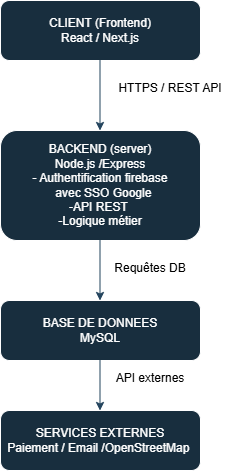
\includegraphics[width=0.50\textwidth]{rapp fig/ARCHI.drawio.png}
    \caption{Architecture de la plateforme }
    \label{fig: Architecture de la plateforme}
\end{figure}
\justifying




La figure précédente illustre l’organisation générale du système ainsi que les interactions existantes entre les différents composants de la plateforme. L’utilisateur interagit avec l’interface frontend via un navigateur web, les requêtes étant ensuite traitées par le serveur backend avant d’être stockées ou récupérées depuis la base de données. Des services externes peuvent également intervenir afin d’enrichir les fonctionnalités proposées




%tableau
\end{spacing}

\section{Diagramme de classes}
\vspace{0.5cm}
\begin{spacing}{1.5}
\justifying
Dans le cadre du projet TravEasy, le diagramme de classes permet de structurer les principales composantes métier du système, notamment la gestion des utilisateurs, des réservations, des paiements, des lieux touristiques ainsi que des avis utilisateurs. Il offre une vision globale et cohérente de l’organisation interne de la plateforme ainsi que des relations entre ses différentes entités.
\end{spacing}
\vspace{0.5cm}
\begin{spacing}{1.5}
\begin{figure}[H]
    \centering
    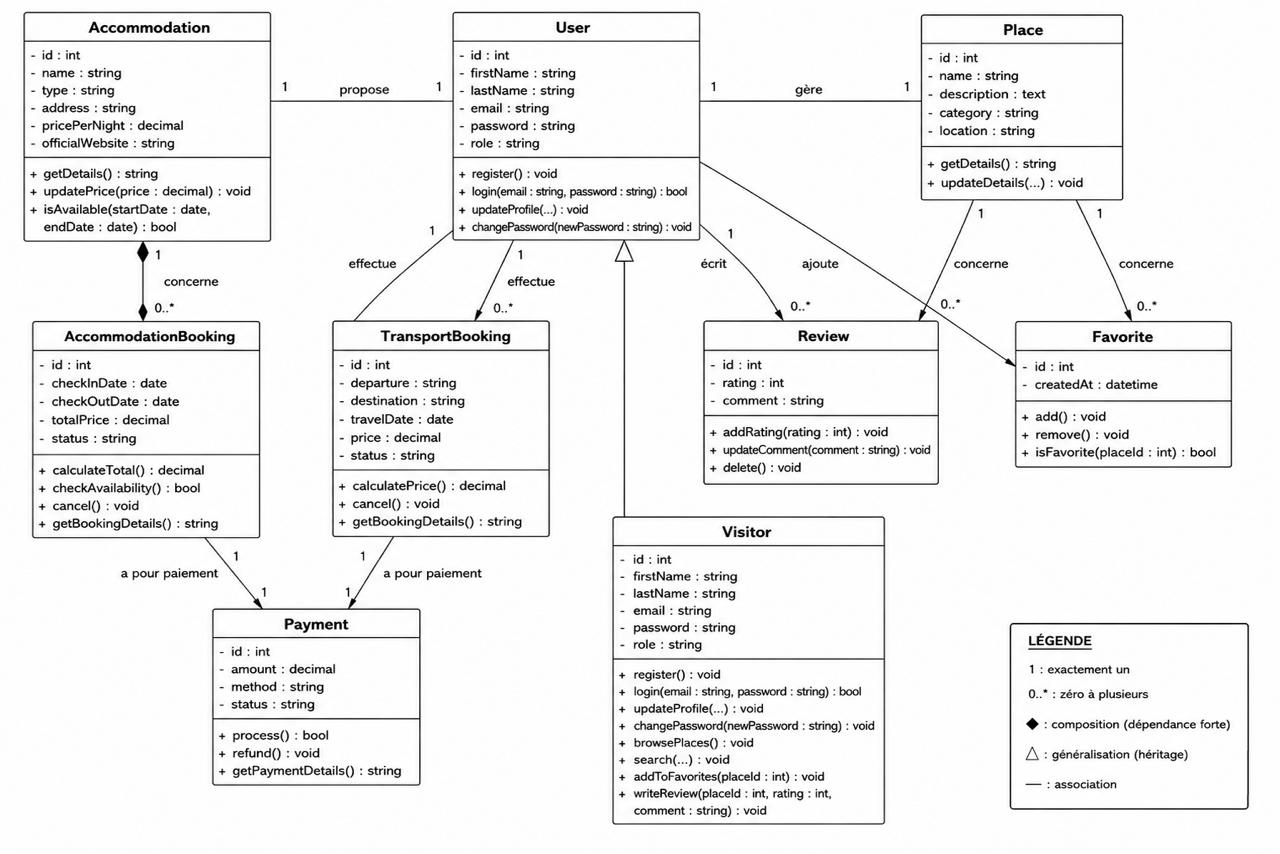
\includegraphics[width=0.7\textwidth]{classe ppt.jpeg}
    \caption{Diagramme de classe  }
    \label{fig: Diagramme de classe }
\end{figure}
\justifying


\end{spacing}
\section{Diagrammes de cas d’utilisation}
\vspace{0.5cm}
\begin{spacing}{1.5}
\justifying
Les diagrammes de cas d’utilisation permettent de représenter les interactions entre les acteurs du système et les fonctionnalités mises à leur disposition. Ils constituent un outil particulièrement utile pour comprendre le comportement attendu du système du point de vue utilisateur. Ils ont été élaborés afin de représenter les principales fonctionnalités offertes aux utilisateurs de la plateforme TravEasy.

\end{spacing}
\subsection{Diagramme de cas d’utilisation global}
\vspace{0.5cm}
\begin{spacing}{1.5}
\justifying
Ce diagramme présente une vue générale des principales interactions entre les utilisateurs et le système.
%
\end{spacing}
\begin{spacing}{1.5}
\begin{figure}[H]
    \centering
    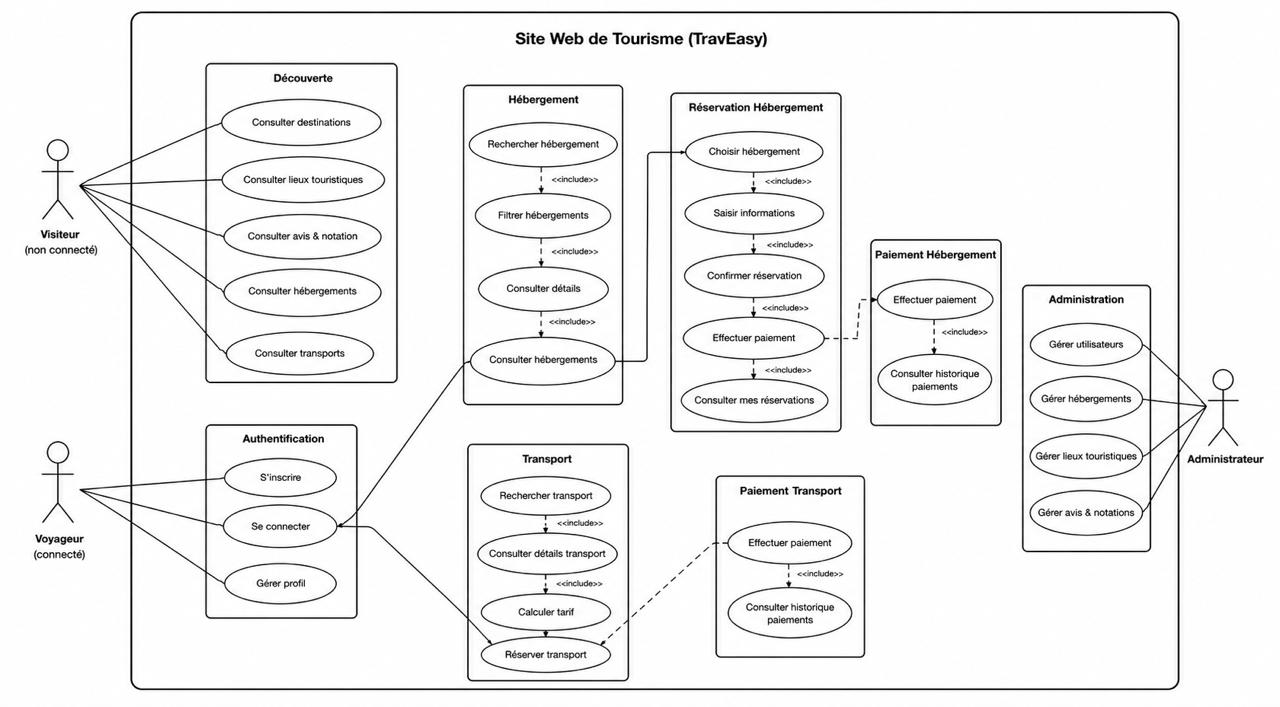
\includegraphics[width=0.5\textwidth]{usecase ppt.jpeg}
    \caption{Diagramme de cas d'utilisation globale  }
    \label{fig: Diagramme de cas d'utilisation globale}
\end{figure}
% \begin{figure}[H]
%     \centering

%     \begin{subfigure}{0.32\textwidth}
%         \centering
%         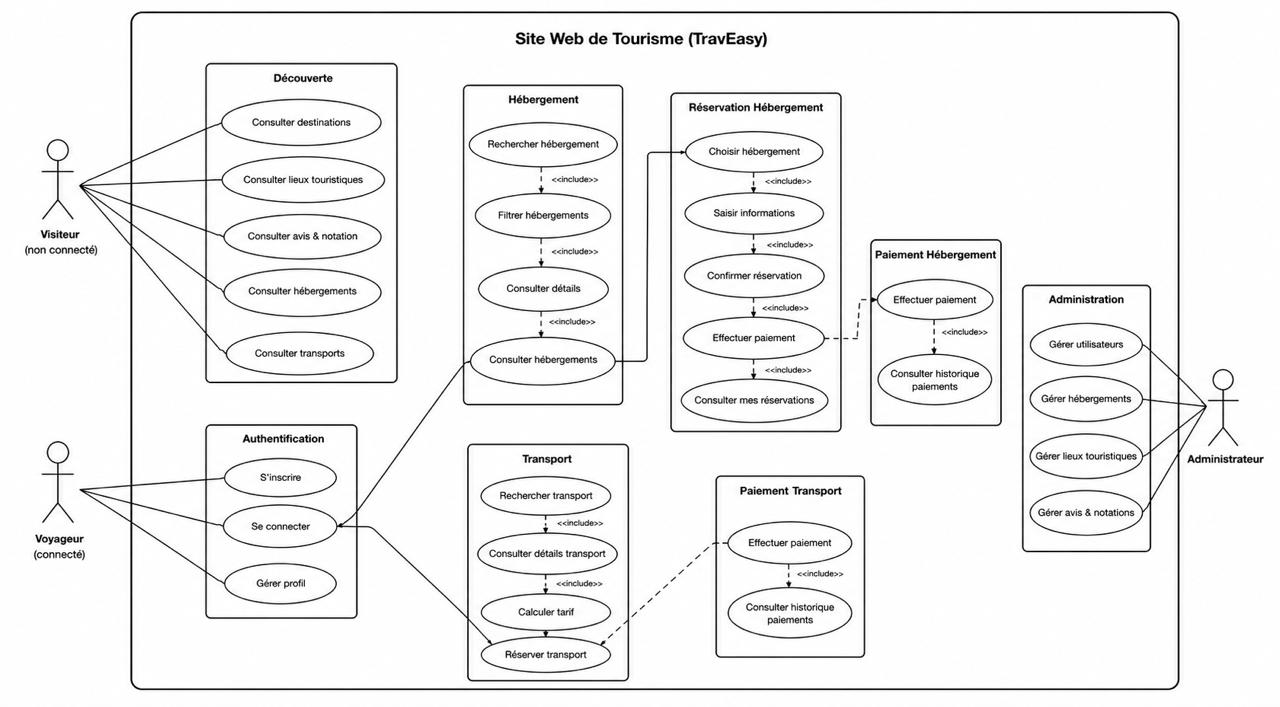
\includegraphics[width=\linewidth]{usecase ppt.jpeg}
%         %\caption{Planning prévisionnel}
%     \end{subfigure}
%     \hfill
%     \begin{subfigure}{0.32\textwidth}
%         \centering
%         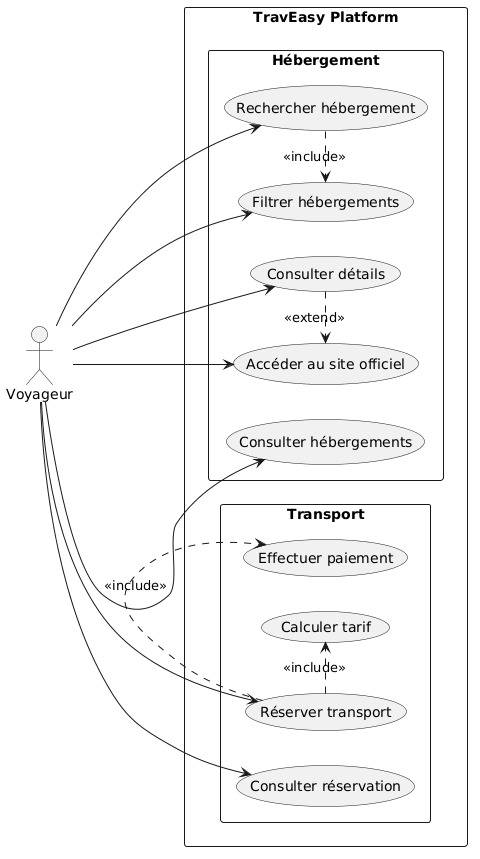
\includegraphics[width=\linewidth]{usecase2.png}
%         %\caption{Planning réel}
%     \end{subfigure}
%     \hfill
%     \begin{subfigure}{0.32\textwidth}
%         \centering
%         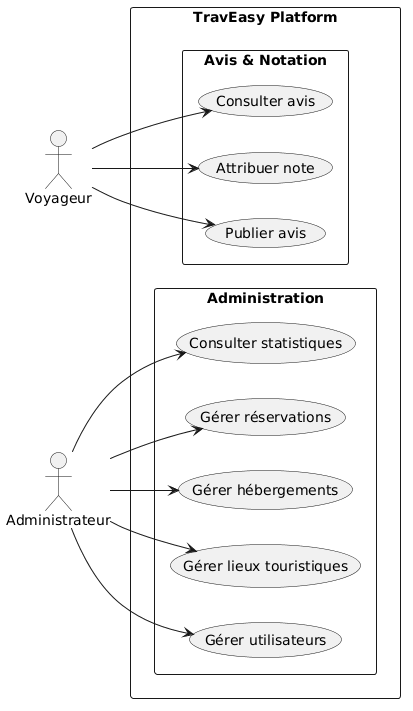
\includegraphics[width=\linewidth]{usecase3.png}
%         %\caption{Analyse des écarts}
%     \end{subfigure}

%     \caption{Diagramme de cas d'utilisation globale}
%     \label{fig:Diagramme de cas d'utilisation globale}
% \end{figure}

Ce diagramme illustre les principales fonctionnalités disponibles au sein de la plateforme, notamment l’authentification, la gestion des réservations, la consultation des contenus touristiques et les opérations de gestion associées.



\end{spacing}
% \subsection{Diagramme de cas d’utilisation du voyageur}
% \vspace{0.5cm}
% \begin{spacing}{1.5}
% \justifying
% Ce diagramme met en évidence les interactions spécifiques du voyageur avec la plateforme.

% \begin{figure}[H]
%     \centering
%     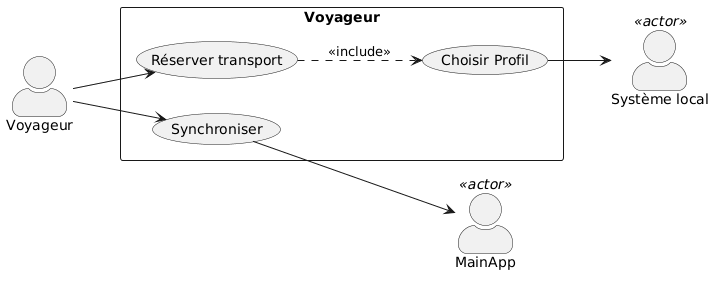
\includegraphics[width=0.5\textwidth]{rapp fig/voyageur usecase.png}
%     \caption{Diagramme de cas d'utilisation voyageur  }
%     \label{fig: Diagramme de cas d'utilisation voyageur}
% \end{figure}
% Le voyageur constitue l’acteur principal du système. Celui-ci peut rechercher des lieux touristiques, réserver un moyen de transport, consulter les informations touristiques disponibles ainsi qu’interagir avec les différents services proposés.
% \end{spacing}

\section{Diagramme d’activité}
\vspace{0.5cm}
\begin{spacing}{1.5}
\justifying

Le diagramme d’activité permet de représenter l’enchaînement logique des opérations exécutées dans un processus fonctionnel donné.

Dans ce projet, un diagramme d’activité a été élaboré afin de modéliser le processus d’authentification.
\begin{figure}[H]
    \centering
    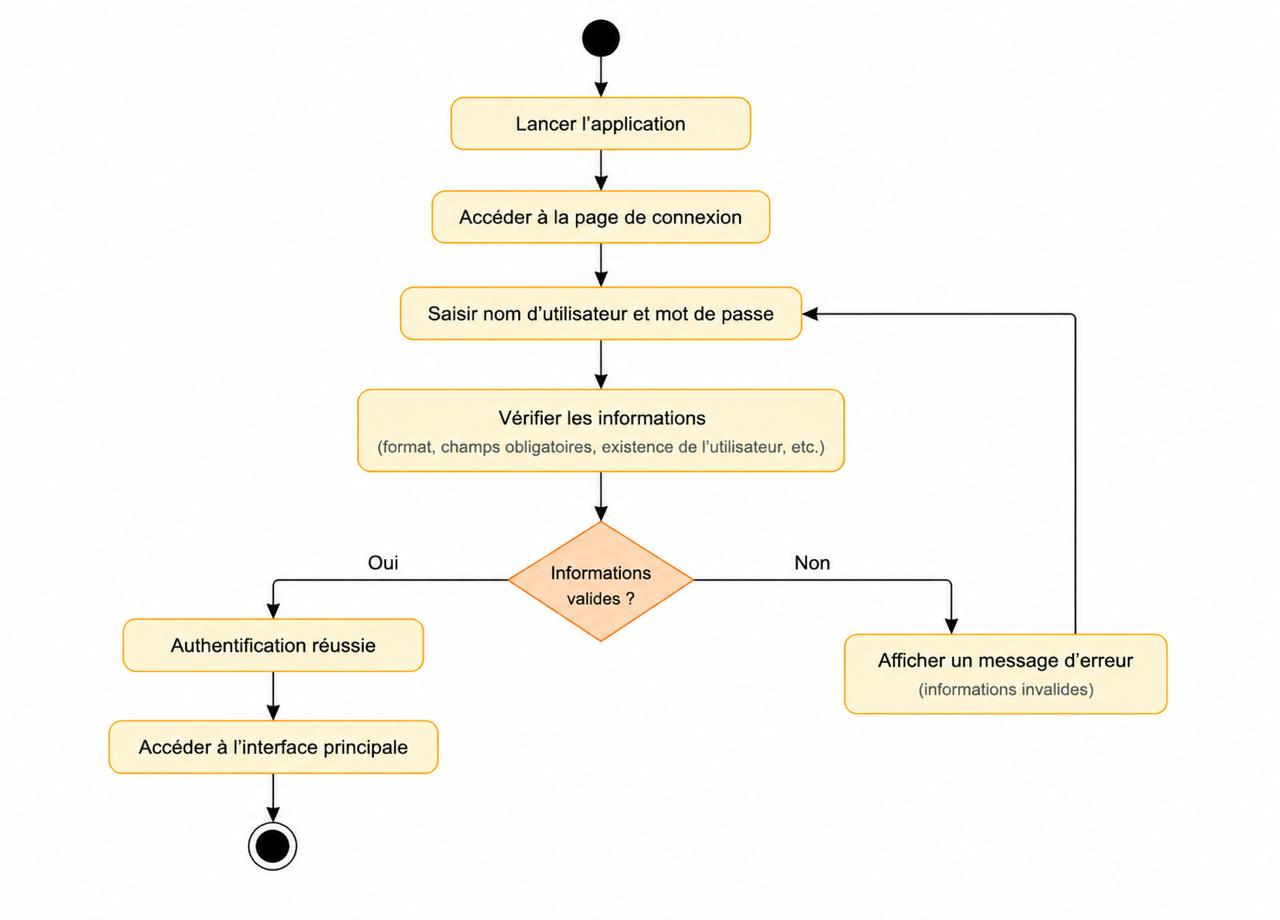
\includegraphics[width=0.5\textwidth]{activite.jpeg}
    \caption{Diagramme d'activité -Authentification   }
    \label{Diagramme d'activité -Authentification }
\end{figure}
Le diagramme précédent illustre les différentes étapes nécessaires au processus d’authentification, depuis la saisie des informations d’identification jusqu’à la validation des accès utilisateur, garantissant ainsi la sécurité du système.


\end{spacing}
\section{Diagrammes de séquence}
\vspace{0.5cm}
\begin{spacing}{1.5}
\justifying
Les diagrammes de séquence permettent de représenter les interactions chronologiques entre les différents composants du système lors de l’exécution d’un scénario fonctionnel.

Ils mettent en évidence les échanges d’informations entre les acteurs, l’interface utilisateur, le backend et la base de données.
\end{spacing}
\subsection{Inscription et authentification}
\vspace{0.5cm}
\begin{spacing}{1.5}
\justifying
Ce scénario décrit le processus permettant à un utilisateur de créer un compte et de s’authentifier afin d’accéder aux fonctionnalités sécurisées de la plateforme.

Scénario : Le voyageur s'inscrit sur la plateforme et se connecte pour accéder aux 
services réservés 
\begin{figure}[H]
    \centering
    \begin{adjustbox}{max width=\textwidth}
    \begin{tikzpicture}[node distance=0cm]
    
      \node[seqpart] at (\CPA,0) {Utilisateur};
      \node[seqpart] at (\CPB,0) {Frontend\\(\texttt{LoginPage})};
      \node[seqpart] at (\CPC,0) {\texttt{AuthController}\\(backend)};
      \node[seqpart] at (\CPD,0) {\texttt{Base de Données}\\(Sequelize)};
    
      \foreach \x in {\CPA,\CPB,\CPC,\CPD}
        \draw[seqlife] (\x,-0.36) -- (\x,-16);
    
      \actbar{\CPA}{-0.36}{-1.9}
      \actbar{\CPB}{-1.9}{-15.2}
      \actbar{\CPC}{-3.1}{-14.0}
      \actbar{\CPD}{-4.3}{-12.5}
      \actbar{\CPA}{-12.8}{-13.3}
    
      \seqF{-0.65}{-0.7}{18.65}{-10.5}{loop}{[tant que identifiants incorrects]}
    
      \seqA{\CPA}{\CPB}{-1.9}{saisit email + mot de passe}
      \seqA{\CPB}{\CPC}{-3.1}{\texttt{POST /auth/login} (email, password)}
      \seqA{\CPC}{\CPD}{-4.3}{\texttt{User.findOne(\{email\})}}
    
      \seqF{\CPB-0.1}{-5.1}{\CPD+0.65}{-8.8}{alt}{[utilisateur non trouvé ou mot de passe incorrect]}
      \seqR{\CPD}{\CPC}{-6.2}{null\,/\,erreur}
      \seqR{\CPC}{\CPB}{-7.0}{\texttt{401} Email ou mot de passe incorrect}
      \seqR{\CPB}{\CPA}{-7.8}{affiche message d'erreur, réinitialise formulaire}
    
      \seqR{\CPD}{\CPC}{-9.5}{user trouvé + hash mdp vérifié}
      \seqR{\CPC}{\CPB}{-10.5}{\texttt{JWT accessToken} + profil utilisateur}
    
      \seqR{\CPB}{\CPA}{-12.0}{redirige vers IHM principale (droits appliqués)}
    
    \end{tikzpicture}
    \end{adjustbox}
    \caption{Diagramme de séquence -- Authentification}
    \label{fig:seq_auth}
    \end{figure}

\end{spacing}

\subsection{Recherche et filtrage de lieux touristiques}
\vspace{0.5cm}
\begin{spacing}{1.5}
\justifying
Ce scénario décrit le fonctionnement du système lors de la recherche d’un lieu touristique selon différents critères de filtrage.
\begin{figure}[H]
    \centering
    \begin{adjustbox}{max width=\textwidth}
    \begin{tikzpicture}[node distance=0cm]
    
      \node[seqpart] at (\CPA,0) {Utilisateur};
      \node[seqpart] at (\CPB,0) {Frontend\\(\texttt{ExplorePage})};
      \node[seqpart] at (\CPC,0) {\texttt{CatalogController}\\(backend)};
      \node[seqpart] at (\CPD,0) {\texttt{CatalogSearchService}\\(SQL)};
      \node[seqpart] at (\CPE,0) {\texttt{Base de Données}\\(\texttt{places})};
    
      \foreach \x in {\CPA,\CPB,\CPC,\CPD,\CPE}
        \draw[seqlife] (\x,-0.36) -- (\x,-22);
    
      \actbar{\CPA}{-0.36}{-1.9}
      \actbar{\CPB}{-1.9}{-21.0}
      \actbar{\CPC}{-3.1}{-20.0}
      \actbar{\CPD}{-4.2}{-10.2}
      \actbar{\CPE}{-5.2}{-9.2}
      \actbar{\CPD}{-13.2}{-16.8}
      \actbar{\CPE}{-14.0}{-15.8}
      \actbar{\CPA}{-19.0}{-19.5}
    
      \seqA{\CPA}{\CPB}{-1.9}{saisit mot-clé, catégorie, localisation, filtres}
      \seqA{\CPB}{\CPC}{-3.1}{\texttt{GET /catalog/suggestions?q=...}}
      \seqA{\CPC}{\CPD}{-4.2}{\texttt{searchSuggestions(query)}}
      \seqA{\CPD}{\CPE}{-5.2}{\texttt{SELECT name FROM places WHERE name LIKE ?}}
      \seqR{\CPE}{\CPD}{-6.2}{liste de noms correspondants}
      \seqR{\CPD}{\CPC}{-7.2}{\{id, name, category\}[]}
      \seqR{\CPC}{\CPB}{-8.2}{suggestions JSON}
      \seqR{\CPB}{\CPA}{-9.0}{affiche liste autocomplete}
    
      \seqA{\CPA}{\CPB}{-10.2}{confirme recherche (filtres: prix, note, openNow, rayon GPS)}
      \seqA{\CPB}{\CPC}{-11.4}{\texttt{GET /catalog/search?category=\&lat=\&lng=\&sortBy=rating}}
      \seqA{\CPC}{\CPD}{-12.5}{\texttt{searchPlaces(filters, sortBy, limit, offset)}}
      \seqA{\CPD}{\CPE}{-13.2}{\texttt{SELECT p.*, distance(Haversine) WHERE filters ORDER BY rating}}
      \seqR{\CPE}{\CPD}{-14.9}{lignes: id, name, category, rating, distance, photos...}
      \seqR{\CPD}{\CPC}{-15.9}{places[] + total + pagination}
      \seqR{\CPC}{\CPB}{-16.9}{\{places, total, page, filters\}}
      \seqR{\CPB}{\CPA}{-17.7}{affiche liste / carte des lieux}
    
      \seqA{\CPA}{\CPB}{-18.8}{clique sur un lieu}
      \seqA{\CPB}{\CPC}{-19.6}{\texttt{GET /catalog/:placeId}}
      \seqR{\CPC}{\CPB}{-20.5}{détails complets + photos + avis + horaires}
      \seqR{\CPB}{\CPA}{-21.3}{affiche fiche lieu}
    
    \end{tikzpicture}
    \end{adjustbox}
    \caption{Diagramme de séquence -- Recherche de lieux touristiques}
    \label{fig:seq_catalog}
    \end{figure}
\end{spacing}
\subsection{Réservation de transport aéroport}
\vspace{0.5cm}
\begin{spacing}{1.5}
\justifying
Ce diagramme modélise les différentes interactions nécessaires à la réservation d’un transport depuis ou vers l’aéroport.
\begin{figure}[H]
    \centering
    \begin{adjustbox}{max width=\textwidth}
    \begin{tikzpicture}[node distance=0cm]
    
      \node[seqpart] at (\CPA,0) {Utilisateur};
      \node[seqpart] at (\CPB,0) {Frontend\\(\texttt{TransportPage})};
      \node[seqpart] at (\CPC,0) {\texttt{TransportController}\\(backend)};
      \node[seqpart] at (\CPD,0) {\texttt{Base de Données}\\(\texttt{transport\_bookings})};
      \node[seqpart] at (\CPE,0) {\texttt{PaymentService}\\(Stripe/CMI)};
    
      \foreach \x in {\CPA,\CPB,\CPC,\CPD,\CPE}
        \draw[seqlife] (\x,-0.36) -- (\x,-23);
    
      \actbar{\CPA}{-0.36}{-2.1}
      \actbar{\CPB}{-2.1}{-22.0}
      \actbar{\CPC}{-3.3}{-21.0}
      \actbar{\CPD}{-4.6}{-7.8}
      \actbar{\CPD}{-11.8}{-15.3}
      \actbar{\CPE}{-13.8}{-17.8}
      \actbar{\CPA}{-20.5}{-21.0}
    
      \seqA{\CPA}{\CPB}{-2.1}{saisit départ, destination, type véhicule, date/heure}
      \seqA{\CPB}{\CPC}{-3.3}{\texttt{GET /transport/estimate} (pickup, dest, vehicleType)}
      \seqA{\CPC}{\CPD}{-4.6}{\texttt{SELECT fare\_config WHERE vehicle\_type = ?}}
      \seqR{\CPD}{\CPC}{-5.7}{tarifs: baseFare, pricePerKm, surcharges...}
      \seqR{\CPC}{\CPB}{-6.7}{estimation: distance, durée, totalFare (MAD)}
      \seqR{\CPB}{\CPA}{-7.5}{affiche récapitulatif tarifaire}
    
      \seqF{-0.65}{-8.4}{25.65}{-11.5}{alt}{[utilisateur confirme la réservation]}
      \seqA{\CPA}{\CPB}{-9.4}{confirme la réservation}
      \seqA{\CPB}{\CPC}{-10.5}{\texttt{POST /transport/book} (JWT + données trajet)}
    
      \seqA{\CPC}{\CPD}{-11.8}{\texttt{INSERT transport\_bookings} (status: pending)}
      \seqR{\CPD}{\CPC}{-12.8}{bookingId généré}
      \seqA{\CPC}{\CPE}{-13.8}{\texttt{createPaymentIntent(totalFare, MAD)}}
      \seqR{\CPE}{\CPC}{-14.9}{paymentClientSecret}
      \seqR{\CPC}{\CPB}{-15.7}{bookingId + paymentClientSecret}
      \seqA{\CPB}{\CPC}{-16.8}{\texttt{POST /payment/confirm} (paymentId)}
    
      \seqF{\CPB-0.1}{-17.6}{\CPE+0.65}{-20.2}{alt}{[paiement accepté] / [paiement refusé]}
      \seqA{\CPC}{\CPD}{-18.5}{\texttt{UPDATE transport\_bookings SET status='assigned'}}
      \seqR{\CPD}{\CPC}{-19.6}{OK}
      \seqR{\CPC}{\CPB}{-20.6}{confirmation + détails chauffeur}
      \seqR{\CPB}{\CPA}{-21.5}{affiche confirmation + numéro réservation}
    
    \end{tikzpicture}
    \end{adjustbox}
    \caption{Diagramme de séquence -- Réservation de transport}
    \label{fig:seq_transport}
    \end{figure}

\end{spacing}
 
\section{Conclusion}
\vspace{0.5cm}
\begin{spacing}{1.5}
\justifying
À travers ce chapitre, les principaux éléments de conception du système ont été présentés afin de fournir une vision structurée du fonctionnement de la plateforme TravEasy. La modélisation UML adoptée a permis de représenter les interactions entre les acteurs, les composants métier ainsi que les scénarios fonctionnels essentiels au bon fonctionnement du système.

Par ailleurs, l’architecture proposée garantit une organisation cohérente des composants applicatifs tout en favorisant la maintenabilité, la modularité et l’évolutivité de la plateforme.

Ainsi, cette phase de conception constitue une base essentielle avant la réalisation technique et l’implémentation des différentes fonctionnalités du système.


\end{spacing}






\newpage
\chapter{ Réalisation et implémentation}
\newpage
\section{Introduction}
\vspace{0.5cm}
\begin{spacing}{1.5}
\justifying
Dans ce chapitre, nous sommes dédiés à la réalisation de la plateforme. Cette étape consiste à mettre en œuvre les modèles de conception dans une application fonctionnelle qui satisfait aux objectifs du projet ainsi qu'aux exigences des utilisateurs. Nous détaillerons l'environnement de développement ainsi que les modules clés créés.

\end{spacing}

\section{Environnement de développement}
\vspace{0.5cm}
\begin{spacing}{1.5}
\justifying

\subsection{Outils logiciels}
\vspace{0.5cm}
\begin{spacing}{1.5}
\justifying
Afin de mener à bien le développement de la plateforme TravEasy, plusieurs outils logiciels ont été utilisés tout au long du projet. Ces outils ont permis d’assurer la conception, le développement, les tests, la gestion des versions ainsi que la modélisation du système. Le tableau suivant présente les principaux outils utilisés et leur rôle dans le projet.

\begin{StdTable}[H]{Outils utilisés dans le projet}{tab:outils}{|X|X|}
\hline
\textbf{Outil} & \textbf{Utilisation} \\ \hline
Visual Studio Code & Développement \\ \hline
Git / GitHub & Gestion des versions \\ \hline
Postman & Test des API \\ \hline
MySQL & Base de données \\ \hline
Draw.io / StarUML & Diagrammes UML \\ \hline
\end{StdTable}

\end{spacing}

\end{spacing}
\section{Choix de l’architecture monolithique}
\vspace{0.5cm}
\begin{spacing}{1.5}
\justifying
\textbf{TravEasy} est une plateforme monolithique constituée d’une grande application structurée en différents modules regroupant les différentes fonctions du système.

Cette décision a été prise pour diverses raisons techniques et organisationnelles.

Tout d’abord, les fonctions de ce système sont étroitement liées entre elles, notamment l’enregistrement des utilisateurs, la réservation, le paiement, les activités touristiques et le transport. Une architecture monolithique permet de les faire communiquer rapidement et de manière fluide sans nécessiter de mécanismes de communication complexes pour le fonctionnement interservices.

De plus, cette approche facilite le développement, les tests, le déploiement et la maintenance de l’application, puisque l’ensemble du système est centralisé dans une seule structure logicielle. Cela permet également de réduire la complexité technique du projet et d’accélérer le cycle de développement.

L’architecture monolithique offre également de bonnes performances pour une plateforme de taille moyenne comme TravEasy, car les échanges internes entre composants s’effectuent localement sans dépendre d’appels réseau supplémentaires.

Le recours à une architecture microservices n’a pas été retenu dans cette première version du projet en raison de la complexité supplémentaire qu’elle introduit, notamment :

la gestion de plusieurs services indépendants ;
la communication entre services via API ;
la gestion distribuée de la sécurité ;
le déploiement de plusieurs serveurs ou conteneurs ;
la supervision des services et la tolérance aux pannes.

Une architecture microservices est généralement plus adaptée aux systèmes de très grande taille nécessitant une forte scalabilité et des équipes de développement importantes.

Toutefois, l’architecture actuelle reste modulaire afin de permettre une éventuelle migration future vers une architecture microservices si les besoins du système évoluent.

\end{spacing}
\section{Choix des technologies utilisées}
\vspace{0.5cm}
\begin{spacing}{1.5}
\justifying

Le choix des technologies utilisées repose sur plusieurs critères, notamment la performance, la flexibilité, la maintenabilité, la rapidité de développement ainsi que la compatibilité avec les applications web modernes.

\subsubsection{Frontend : React.js et Next.js}

React.js a été choisi pour le développement du frontend grâce à son architecture basée sur des composants réutilisables, permettant de concevoir des interfaces dynamiques, interactives et faciles à maintenir. Cette technologie offre une grande flexibilité, de bonnes performances grâce au Virtual DOM et une importante communauté de développeurs. Comparé à Angular, dont l’architecture est plus complexe et plus lourde à mettre en œuvre, React répond mieux aux besoins du projet en offrant une plus grande simplicité de développement. Bien que Vue.js constitue également une alternative performante, React bénéficie d’un écosystème plus mature et d’une adoption plus large dans le développement d’applications web modernes.

\subsubsection{Backend : Node.js et Express.js} 

Le backend repose sur Node.js associé au framework Express.js. Ce choix s’explique par le modèle asynchrone de Node.js, qui permet de gérer efficacement un grand nombre de requêtes simultanées tout en offrant d’excellentes performances. L’utilisation de JavaScript aussi bien côté client que côté serveur assure également une cohérence technologique au sein du projet. Quant à Express.js, il a été retenu pour sa légèreté, sa simplicité et sa capacité à faciliter le développement d’API REST. Des solutions telles que Spring Boot ou Django ont été envisagées, mais elles nécessitent une configuration plus importante et présentent une courbe d’apprentissage plus élevée pour les besoins de cette plateforme.

\subsubsection{Base de données : MySQL 8}

Pour la gestion des données, MySQL 8 a été retenu comme système de gestion de base de données relationnelle. Ce choix repose sur sa robustesse, sa fiabilité et sa compatibilité avec l’environnement Node.js. De plus, la nature des données manipulées dans le projet implique de nombreuses relations entre les utilisateurs, les réservations, les paiements et les activités touristiques, ce qui rend le modèle relationnel particulièrement adapté. Contrairement à certaines bases de données NoSQL, MySQL garantit une meilleure cohérence des données et une gestion efficace des relations complexes, tout en offrant d’excellentes performances et une administration simplifiée.

\subsubsection{APIs externes : Firebase, Open Street Map, Stripe et PayPal}

La plateforme intègre plusieurs APIs externes afin d’enrichir ses fonctionnalités. 
Firebase avec SSO google a été choisi pour la gestion de l’authentification en raison de sa simplicité d’intégration, de sa sécurité renforcée.  
Open Street Map a été choisie pour sa précision, sa couverture géographique mondiale et ses fonctionnalités avancées de géolocalisation et de cartographie. Pour les paiements en ligne, Stripe et PayPal ont été retenus en raison de leur fiabilité, de leur niveau élevé de sécurité et de leur large adoption dans le commerce électronique. Le recours à ces solutions permet de bénéficier de services éprouvés et régulièrement mis à jour, évitant ainsi le développement de fonctionnalités complexes tout en garantissant une meilleure expérience utilisateur.
\end{spacing}

\section{Implémentation de la base de données}
\vspace{0.5cm}
\begin{spacing}{1.5}
\justifying
La base de données de la plateforme a été implémentée à l’aide de MySQL 8 conformément au modèle de données défini lors de la phase de conception. Elle assure le stockage et la gestion des informations relatives aux utilisateurs, aux lieux touristiques, aux hébergements , aux réservations de transport ainsi qu’aux transactions de paiement. Les principales tables de la base de données sont présentées ci-dessous.
\begin{itemize}
    \item \textbf{Table User}
\end{itemize}

Cette table stocke les informations relatives aux utilisateurs de la plateforme, notamment leurs identifiants de connexion et leur rôle au sein du système.

\begin{StdTable}[H]{Table Utilisateur}{tab:utilisateur}{|X|X|}
\hline
\textbf{Champ} & \textbf{Type} \\ \hline
id & INT \\ \hline
email & VARCHAR \\ \hline
password & VARCHAR \\ \hline
role & VARCHAR \\ \hline
\end{StdTable}
\begin{itemize}
    \item \textbf{Table Place}
\end{itemize}

La table \textbf{Place} contient les informations concernant les lieux touristiques référencés sur la plateforme.

\begin{StdTable}[H]{Table Point d'intérêt}{tab:point_interet}{|X|X|}
\hline
\textbf{Champ} & \textbf{Type} \\ \hline
id & INT \\ \hline
name & VARCHAR \\ \hline
category & VARCHAR \\ \hline
description & TEXT \\ \hline
latitude & FLOAT \\ \hline
longitude & FLOAT \\ \hline
\end{StdTable}
\begin{itemize}
    \item \textbf{Table TransportBooking}
\end{itemize}

Cette table permet d’enregistrer les réservations de transport effectuées par les utilisateurs ainsi que les informations nécessaires au calcul du tarif.

\begin{StdTable}[H]{Table Estimation de trajet}{tab:estimation_trajet}{|X|X|}
\hline
\textbf{Champ} & \textbf{Type} \\ \hline
pickup & VARCHAR \\ \hline
dropoff & VARCHAR \\ \hline
distanceKm & FLOAT \\ \hline
calculatedPrice & FLOAT \\ \hline
\end{StdTable}
\begin{itemize}
    \item \textbf{Table Payment}
\end{itemize}

La table \textbf{Payment} assure le suivi des transactions financières réalisées sur la plateforme.

\begin{StdTable}[H]{Table Paiement}{tab:paiement}{|X|X|}
\hline
\textbf{Champ} & \textbf{Type} \\ \hline
amount & FLOAT \\ \hline
method & VARCHAR \\ \hline
status & VARCHAR \\ \hline
\end{StdTable}
\begin{itemize}
    \item \textbf{Table Accommodation}
\end{itemize}

La table \textbf{Accommodation} stocke les informations relatives aux différents hébergements proposés sur la plateforme, tels que les hôtels, les riads, les auberges et les maisons d’hôtes. Elle permet d’effectuer les recherches et les filtrages selon plusieurs critères, notamment la ville, le type d’établissement, le nombre d’étoiles et la gamme de prix.

\begin{StdTable}[H]{Table Hébergement}{tab:hebergement}{|X|X|}
\hline
\textbf{Champ} & \textbf{Type} \\ \hline
id & INT \\ \hline
name & VARCHAR \\ \hline
type & VARCHAR \\ \hline
city & VARCHAR \\ \hline
stars & INT \\ \hline
priceRange & VARCHAR \\ \hline
description & TEXT \\ \hline
websiteUrl & VARCHAR \\ \hline
\end{StdTable}

%les tables 
%capture decrand d base de donnees

\end{spacing}

\section{Réalisation des modules fonctionnels}
\vspace{0.5cm}
\begin{spacing}{1.5}
\justifying

\newpage
\subsection{Page d’accueil de la plateforme}
\vspace{0.5cm}
\begin{spacing}{1.5}
\justifying
La page d’accueil constitue le point d’entrée principal de la plateforme TravEasy. Elle a été conçue pour offrir aux utilisateurs un accès rapide et intuitif aux différentes fonctionnalités disponibles. Cette interface met en avant les principaux services proposés, notamment la consultation des destinations touristiques, la recherche d’hébergements, la réservation de transport ainsi que l’accès aux avis des utilisateurs. La figure suivante présente l’interface d’accueil développée dans le cadre du projet.
\begin{figure}[H]
\centering
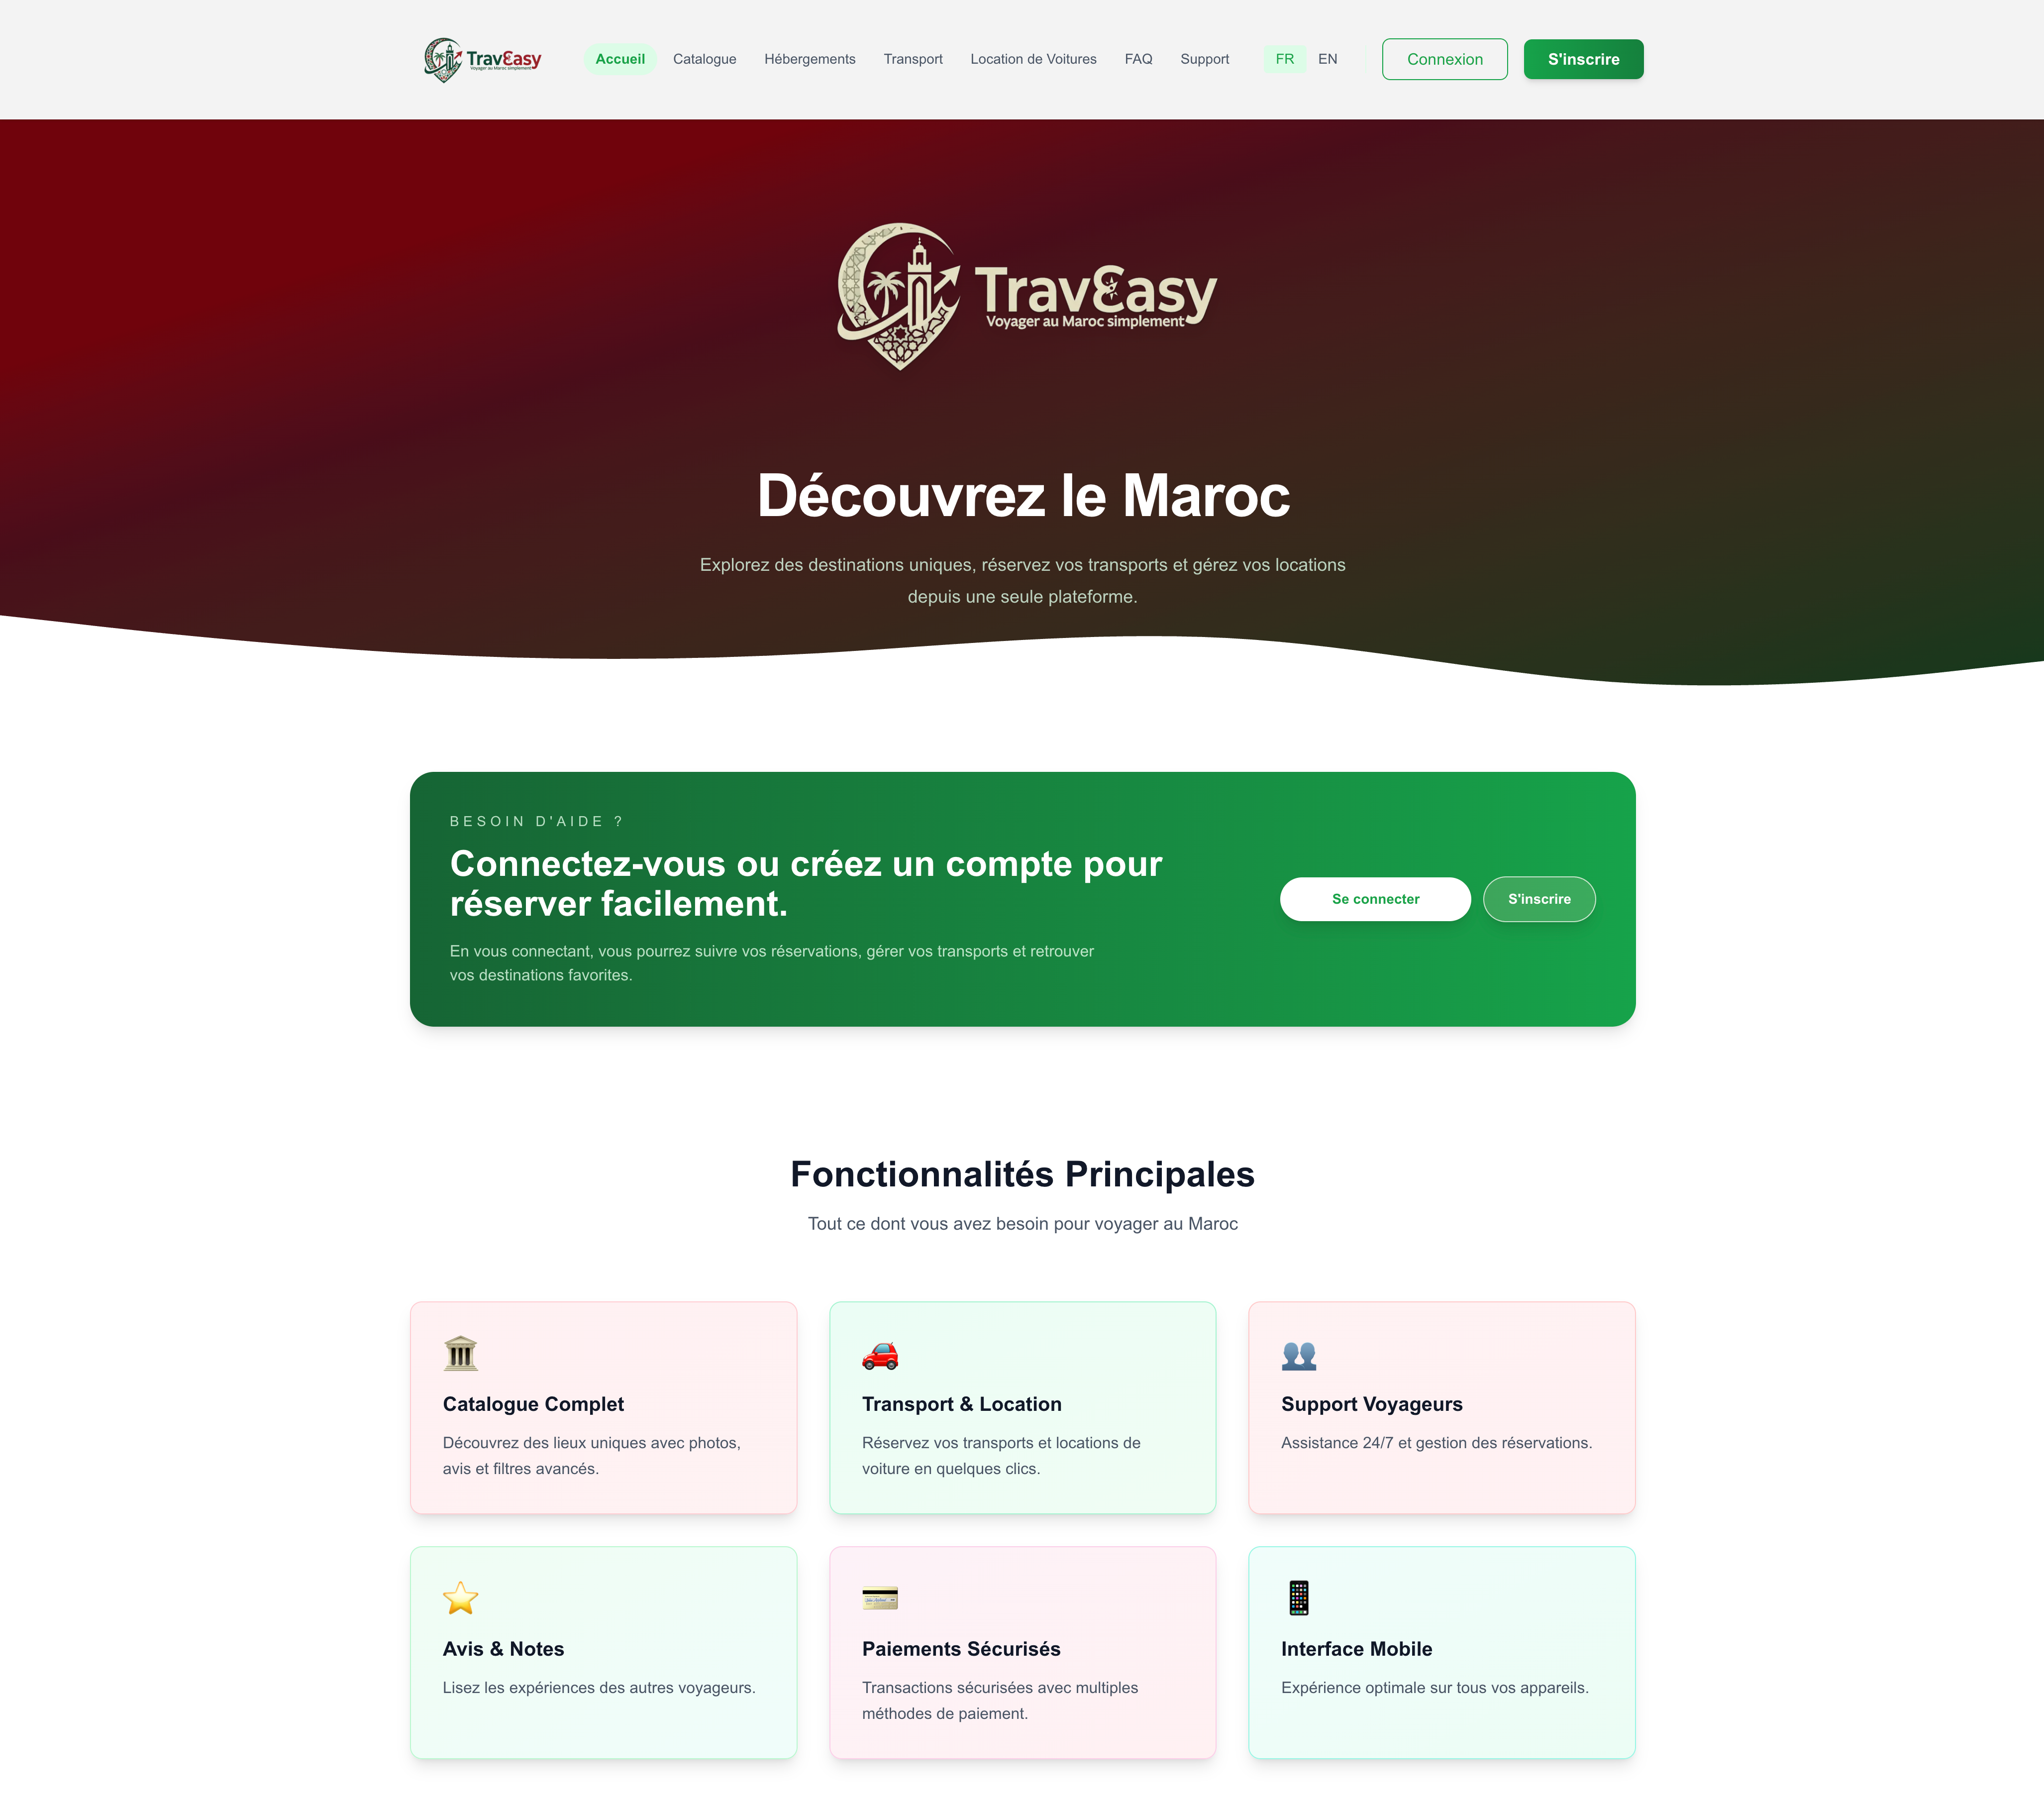
\includegraphics[width=\textwidth]{home1.png}
\caption{Page d'accueil avant la connexion}
\label{fig:Page d'accueil avant la connexion}
\end{figure}

La page d'accueil constitue le point d'entrée principal de la plateforme TravEasy. Elle offre un accès rapide et intuitif aux différentes fonctionnalités disponibles, notamment la consultation des destinations touristiques, la recherche d'hébergements, la réservation de transport et l'accès aux avis des utilisateurs.

\begin{figure}[H]
\centering
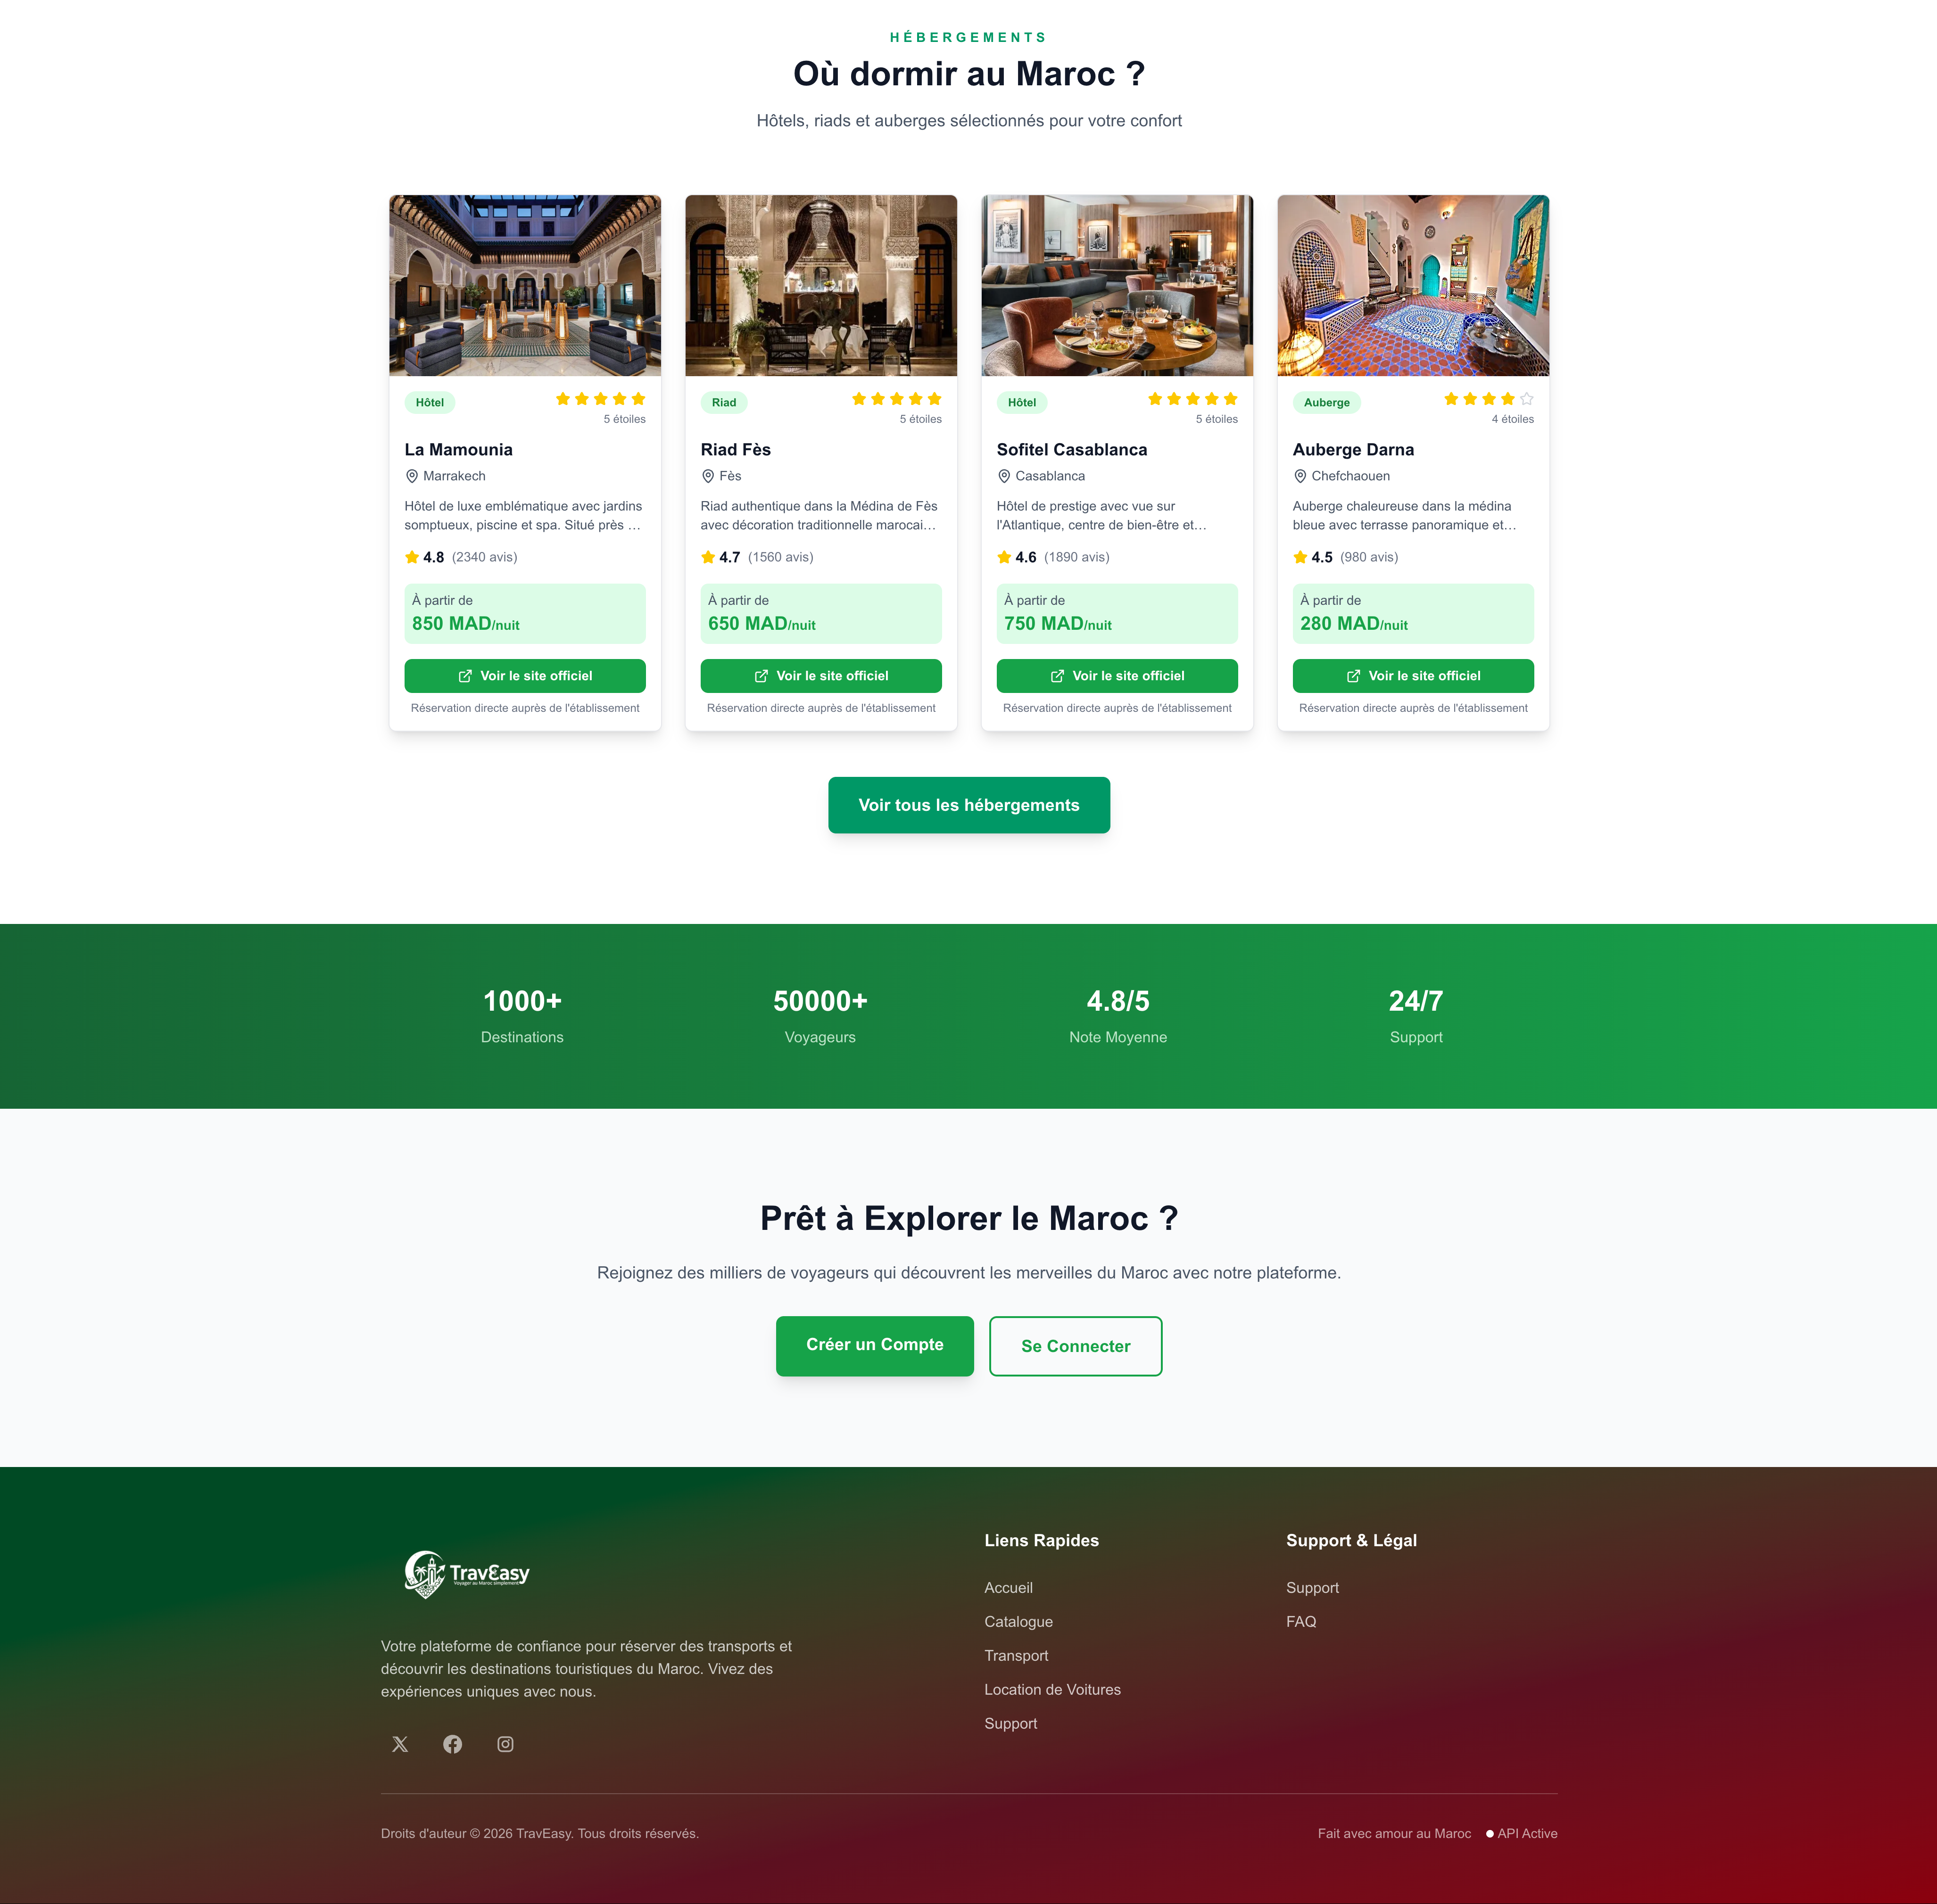
\includegraphics[width=\textwidth]{home2.png}
\caption{Suite page d'accueil avant la connexion}
\label{fig:Suite page d'accueil avant la connexion}
\end{figure}

Cette vue présente la suite de la page d'accueil, complétant la présentation des services et fonctionnalités proposés par la plateforme avant toute connexion de l'utilisateur.


\begin{figure}[H]
\centering
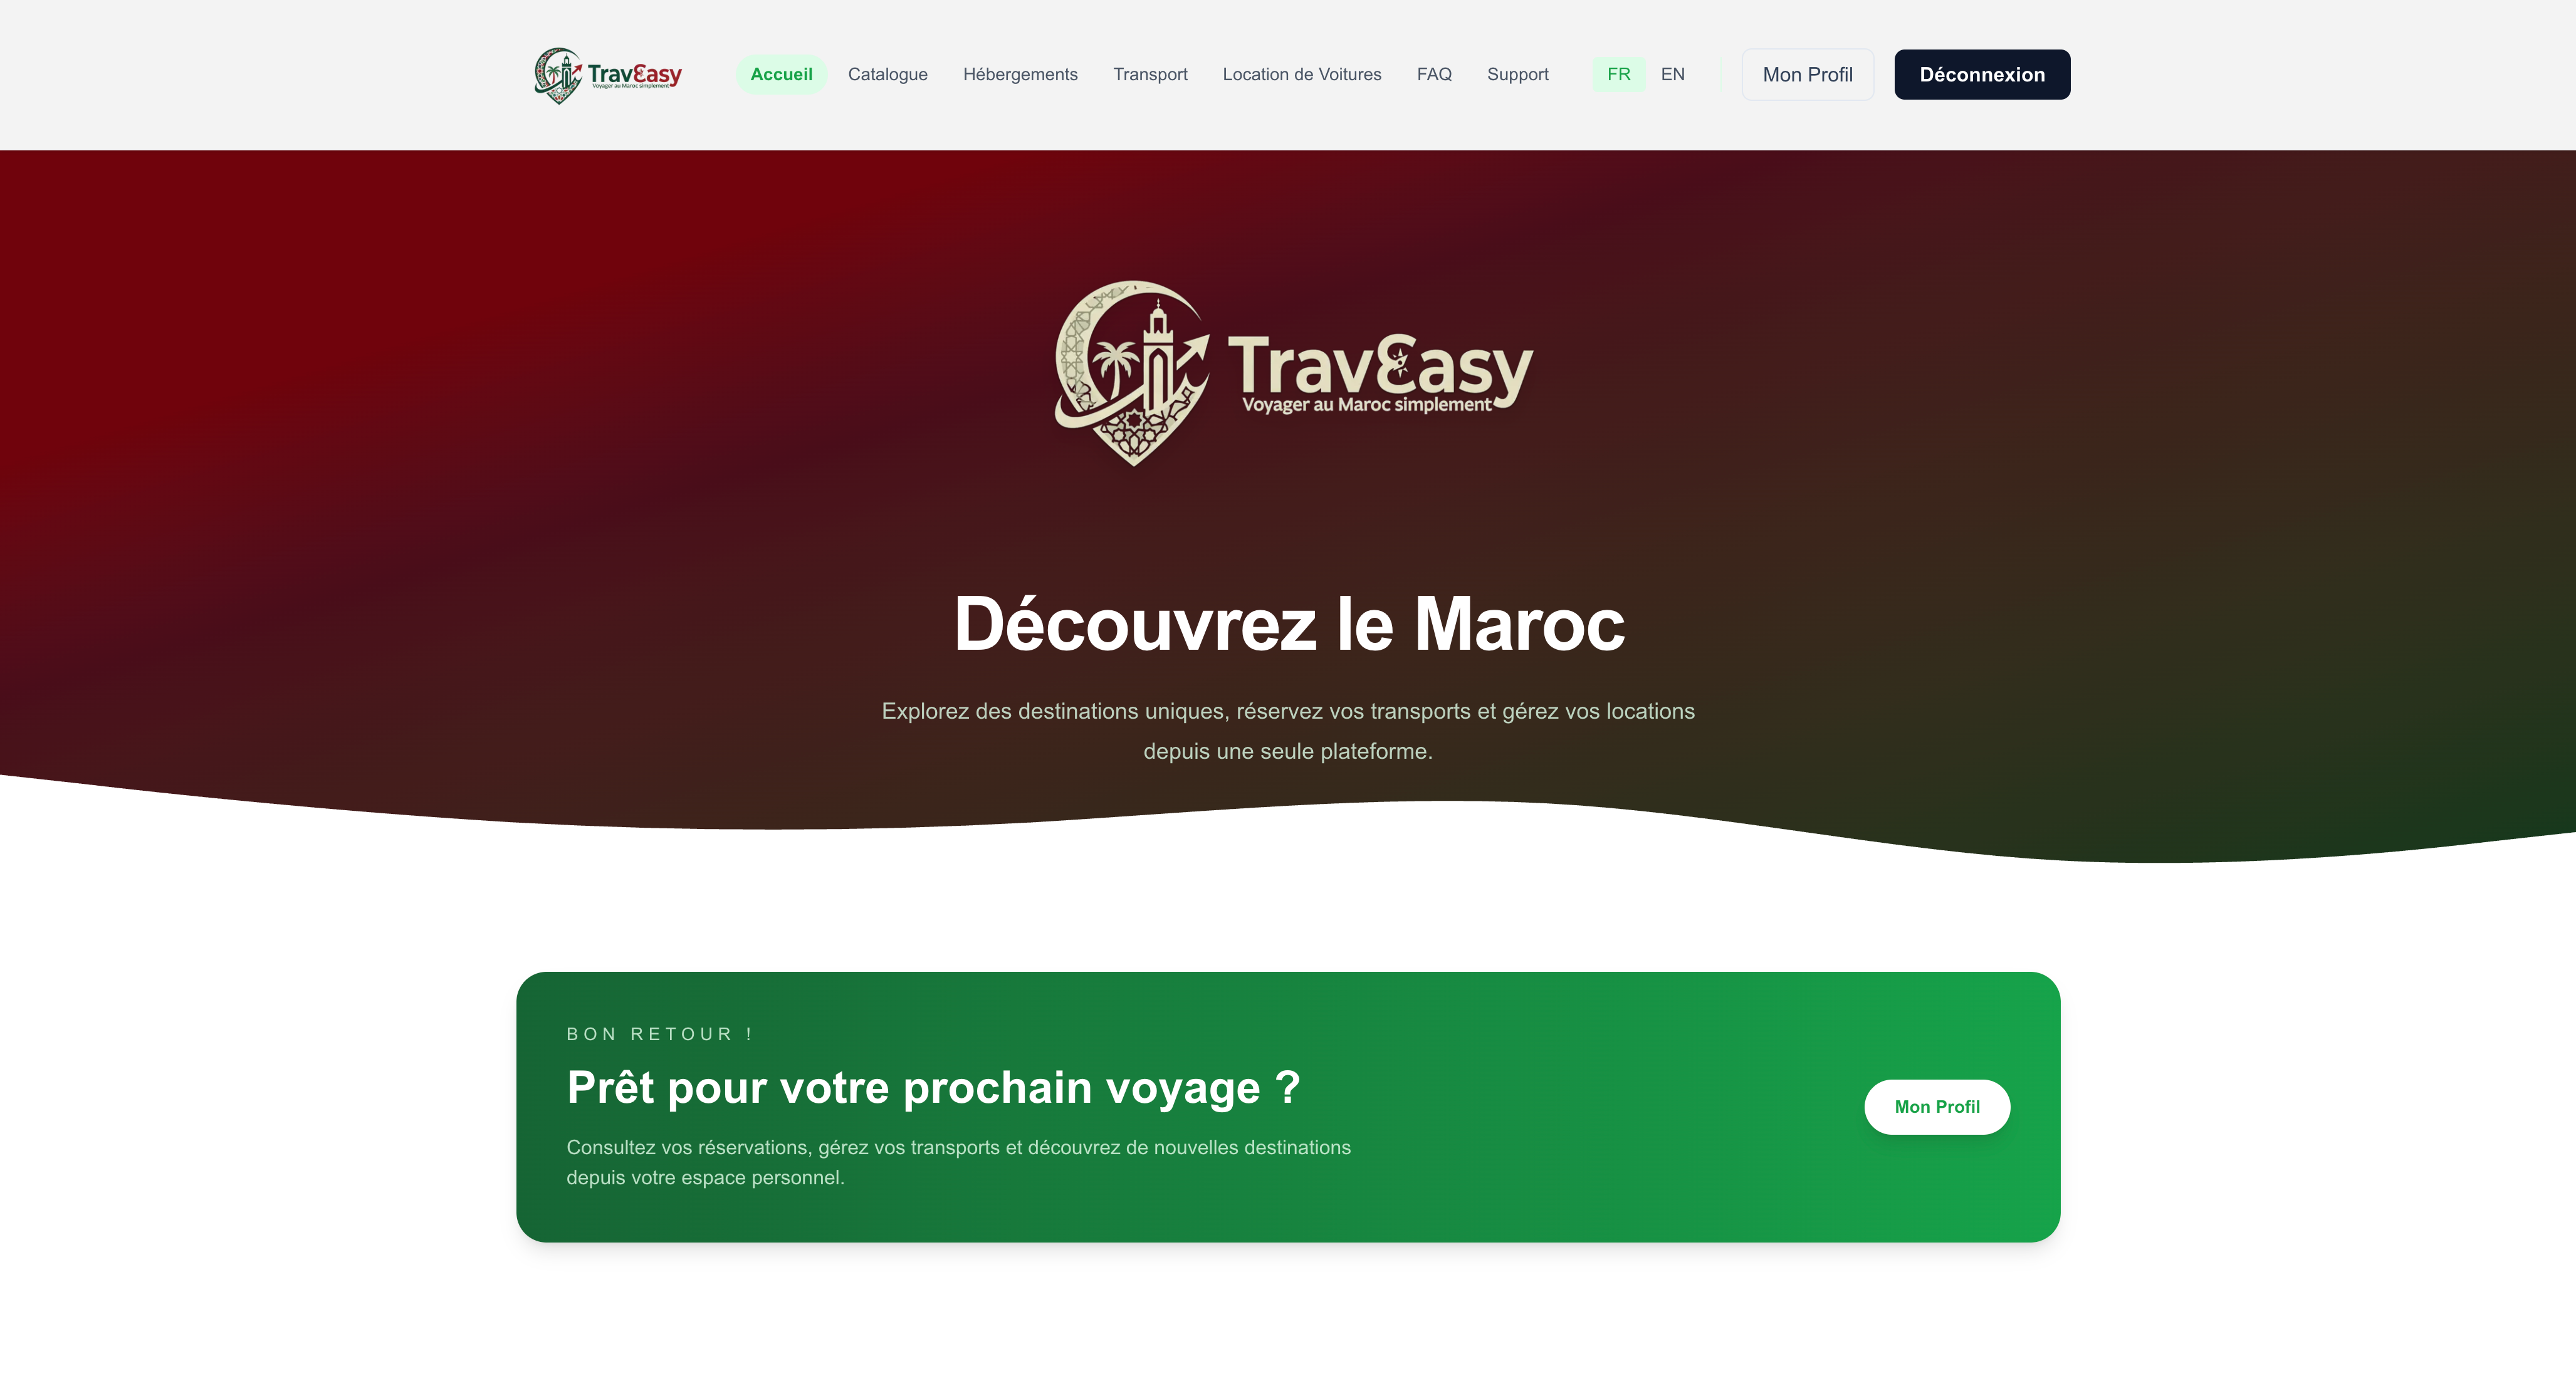
\includegraphics[width=\textwidth]{home log in.png}
\caption{Page d'accueil après la connexion}
\label{fig:Page d'accueil apres la connexion}
\end{figure}

Une fois connecté, l'utilisateur accède à une interface d'accueil personnalisée lui permettant de naviguer directement vers l'ensemble des fonctionnalités de la plateforme selon son profil et ses préférences.


\begin{figure}[H]
\centering
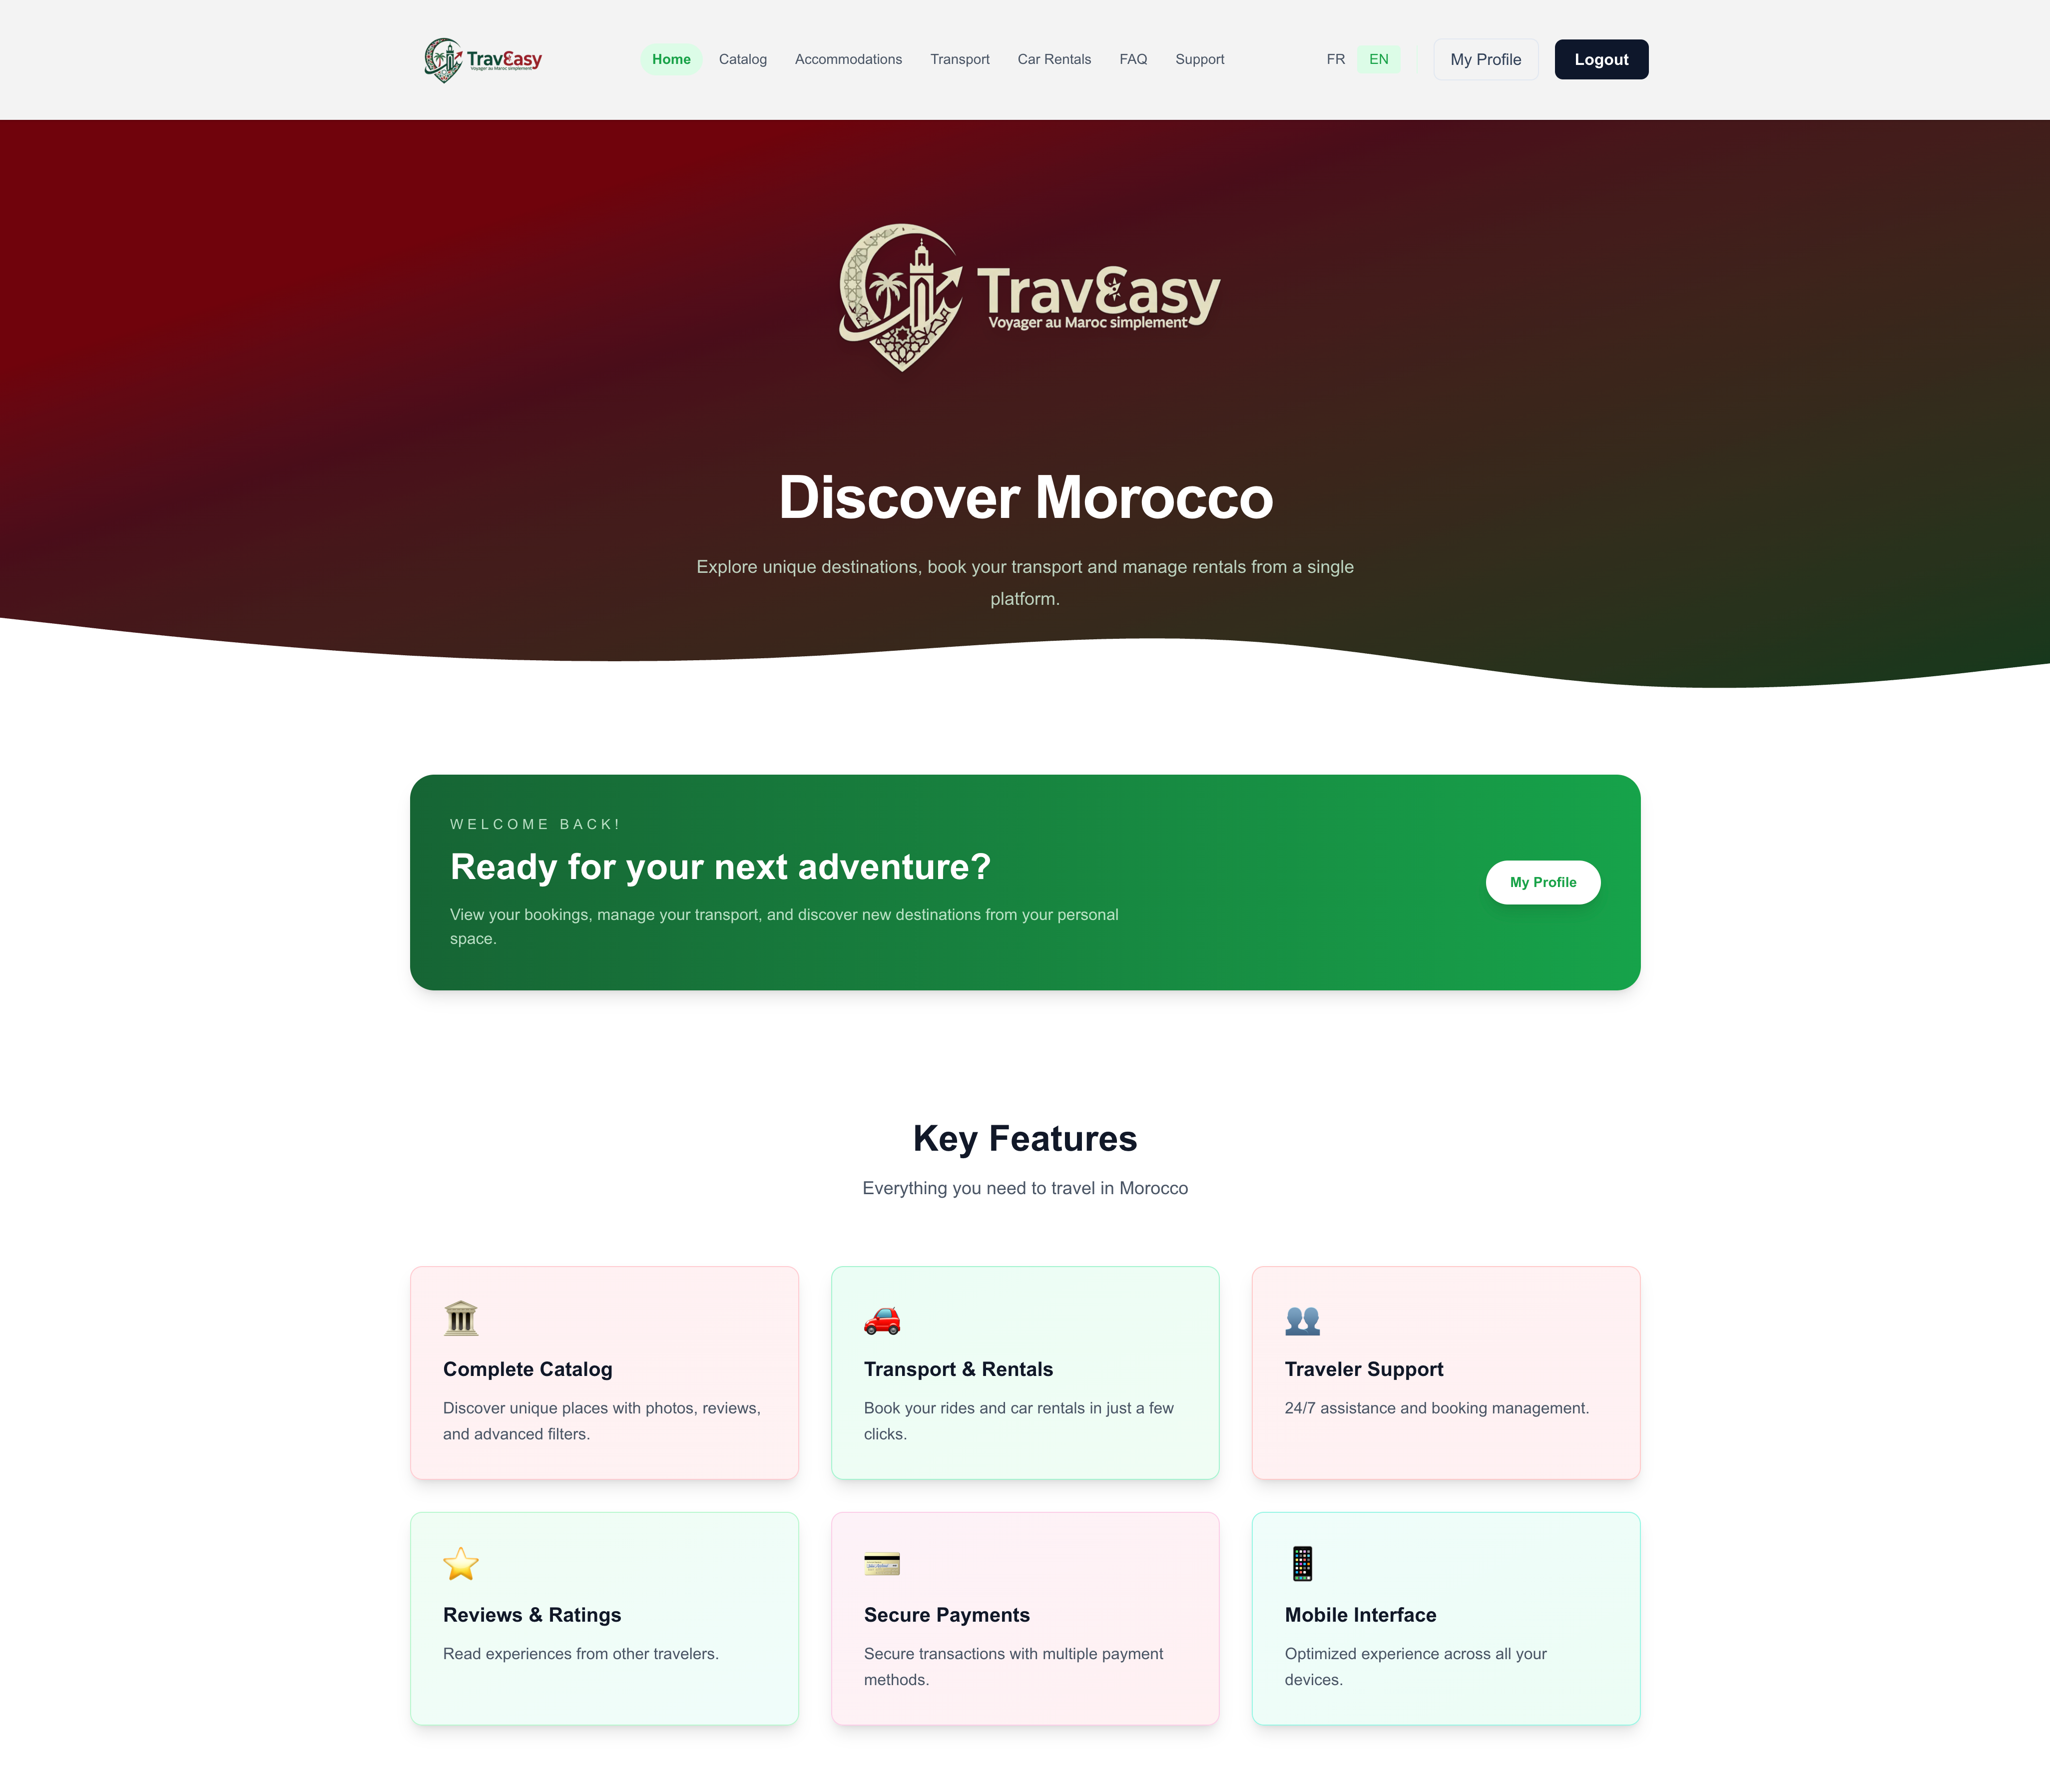
\includegraphics[width=\textwidth]{home1 en.png}
\caption{Page d'accueil en anglais}
\label{fig:Page d'accueil en anglais}
\end{figure}

La plateforme TravEasy intègre un support multilingue. Cette figure illustre l'interface d'accueil affichée en langue anglaise, permettant d'élargir l'accessibilité de la plateforme à un public international.

\begin{figure}[H]
\centering
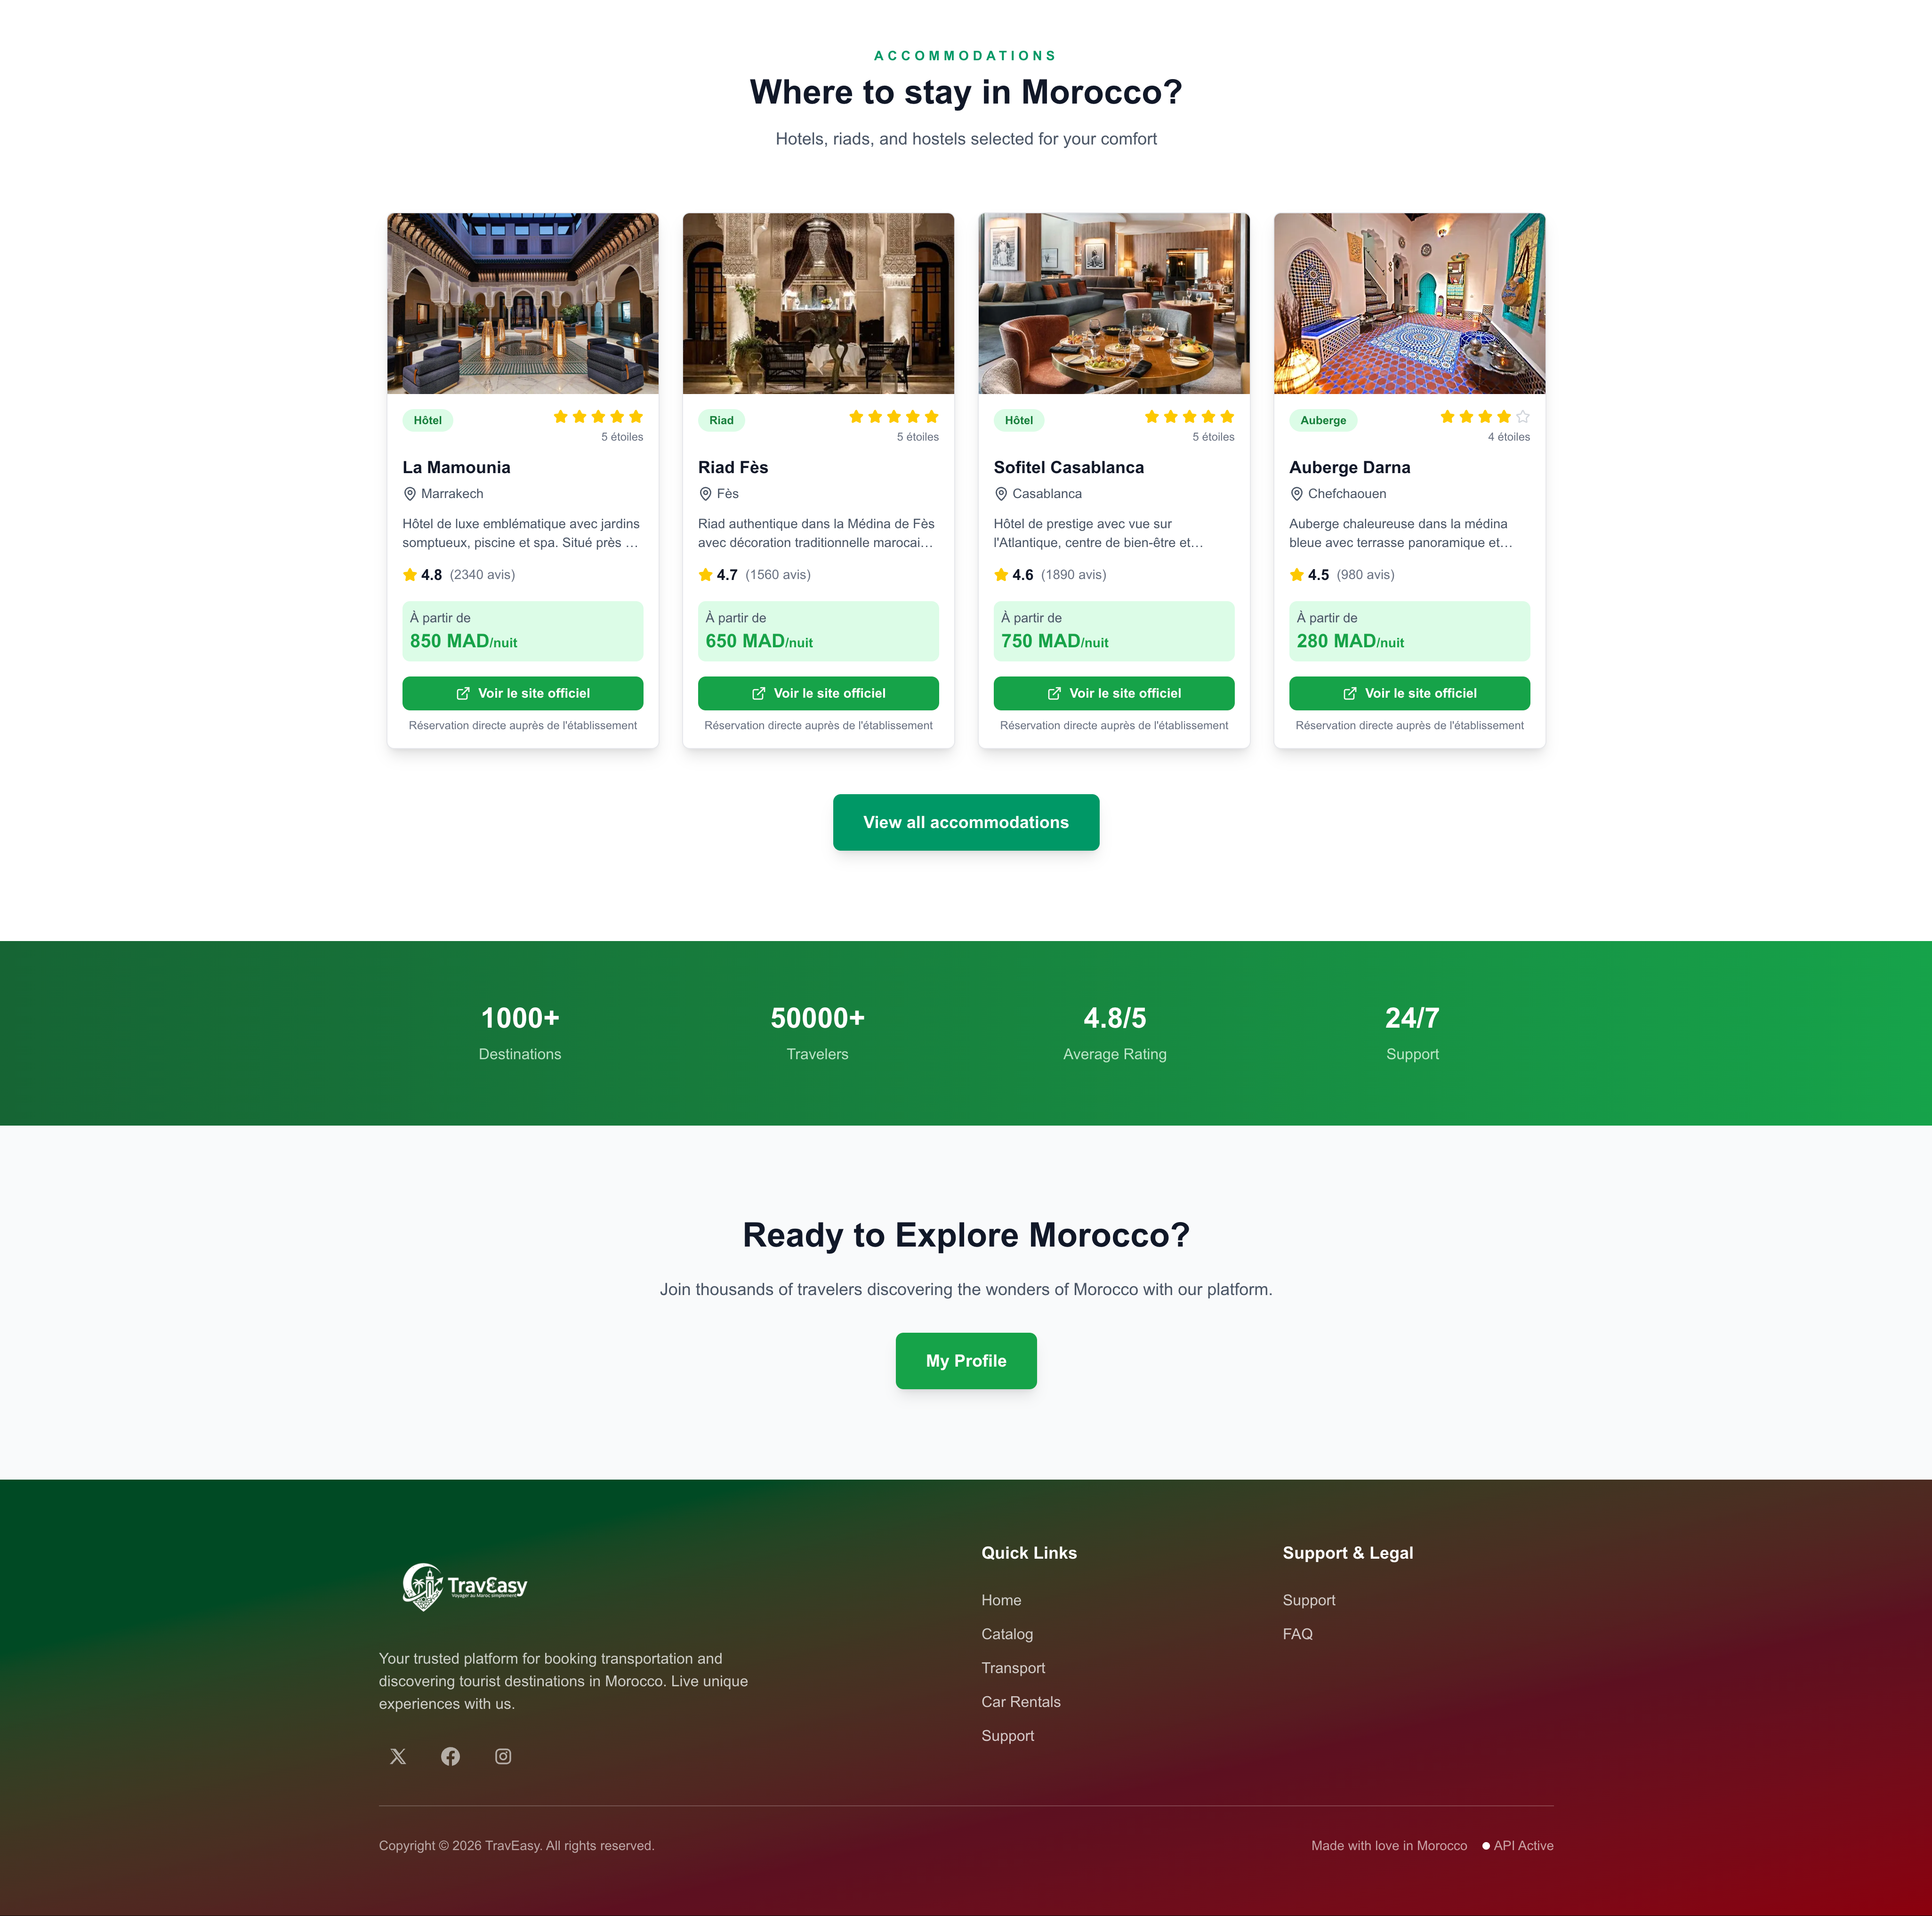
\includegraphics[width=\textwidth]{home2 en.png}
\caption{Suite page d'accueil en anglais}
\label{fig:Suite page d'accueil en anglais}
\end{figure}

Cette vue présente la suite de la page d'accueil en version anglaise, confirmant la prise en charge complète du multilingue sur l'ensemble du contenu de l'interface.

\end{spacing}

\subsection{Module d'authentification}
\vspace{0.5cm}
\begin{spacing}{1.5}
\justifying
Le module d’authentification constitue la première couche de sécurité de la plateforme. 
Il permet aux utilisateurs de créer un compte à travers la fonctionnalité d’\textbf{inscription} et d’accéder à leurs espaces personnels via la \textbf{connexion}. 
Afin de garantir la sécurité des échanges et la protection des données, l’authentification repose sur l’utilisation du module \textbf{Firebase} soit via un formulaire soit via \textbf{SSO Google}, ce qui assure une gestion sécurisée des sessions utilisateur. 
Ce module intègre également un mécanisme de \textbf{gestion des rôles}, permettant de définir différents niveaux d’accès et d’autorisation selon le profil de l’utilisateur (administrateur, utilisateur standard, etc.). 
Cette approche garantit un contrôle efficace des ressources et des fonctionnalités accessibles au sein de la plateforme.

%Capture écran formulaire inscription
\begin{figure}[H]
\centering
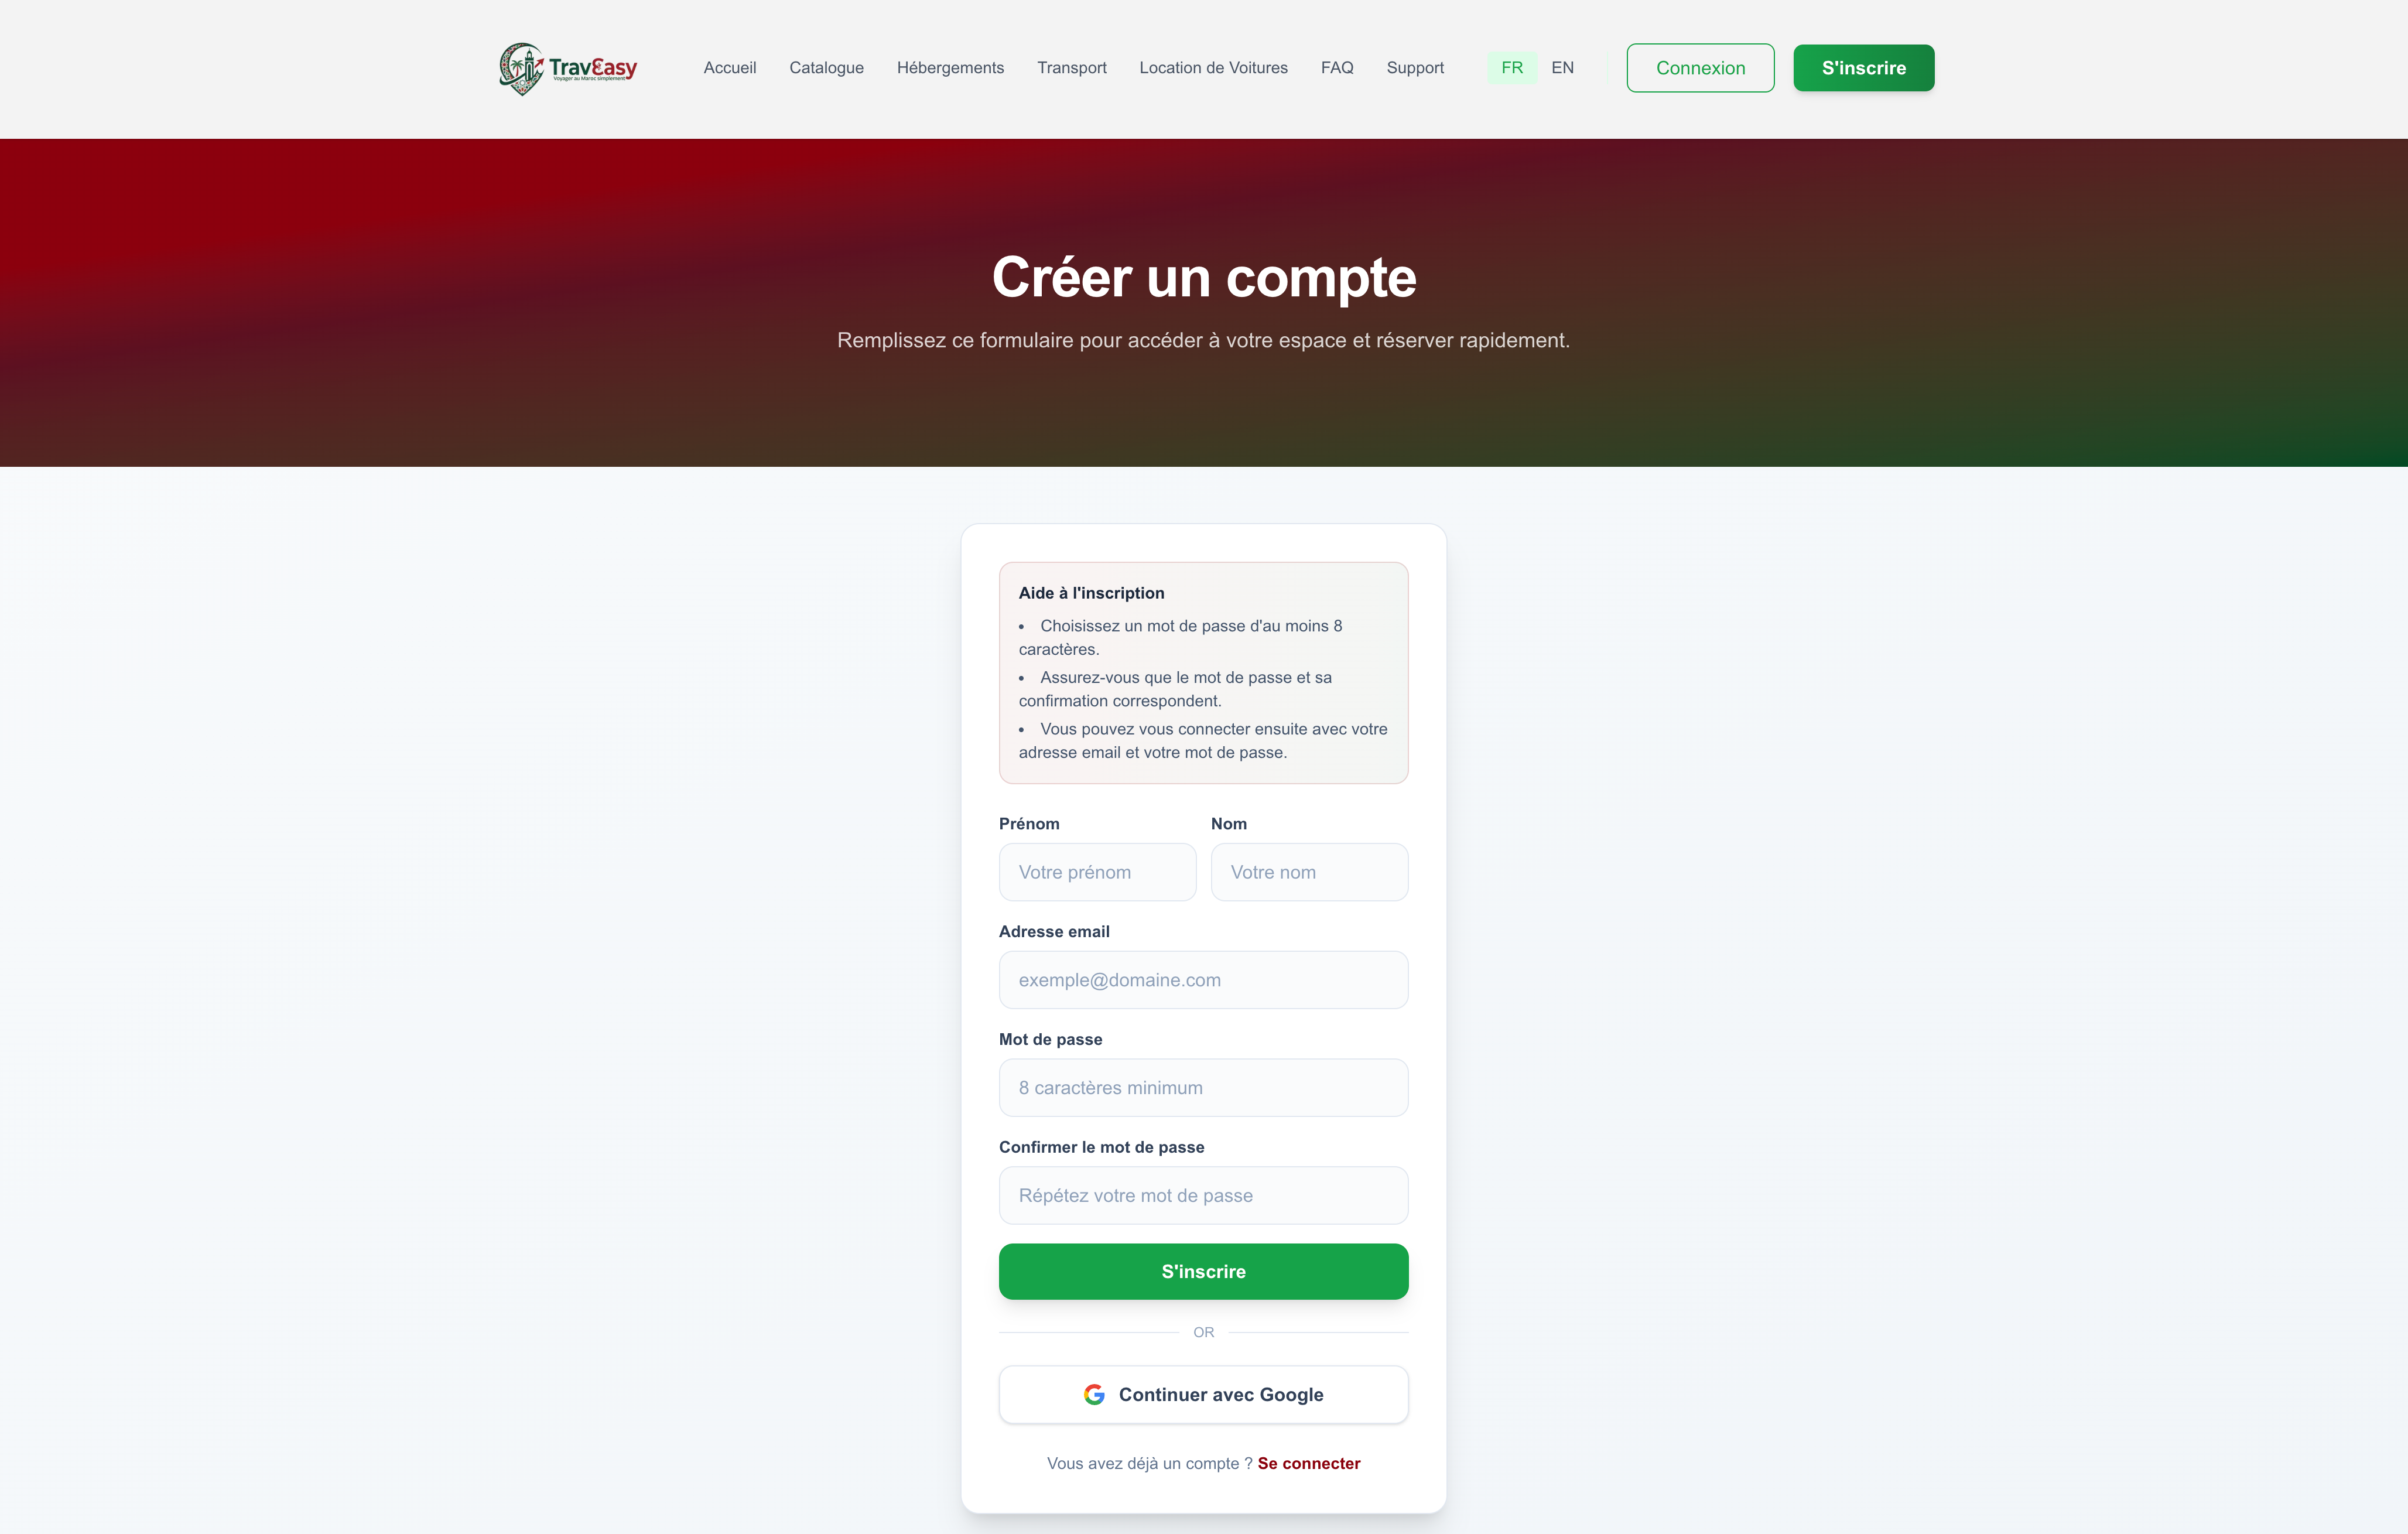
\includegraphics[width=\textwidth]{signup.png}
\caption{Formulaire d'inscription}
\label{fig:Formulaire d'inscription}
\end{figure}

Le formulaire d'inscription permet aux nouveaux utilisateurs de créer un compte sur la plateforme, soit via un formulaire classique, soit via l'authentification SSO Google, garantissant ainsi une prise en main simple et sécurisée grâce à Firebase.

%Capture écran connexion

\begin{figure}[H]
\centering
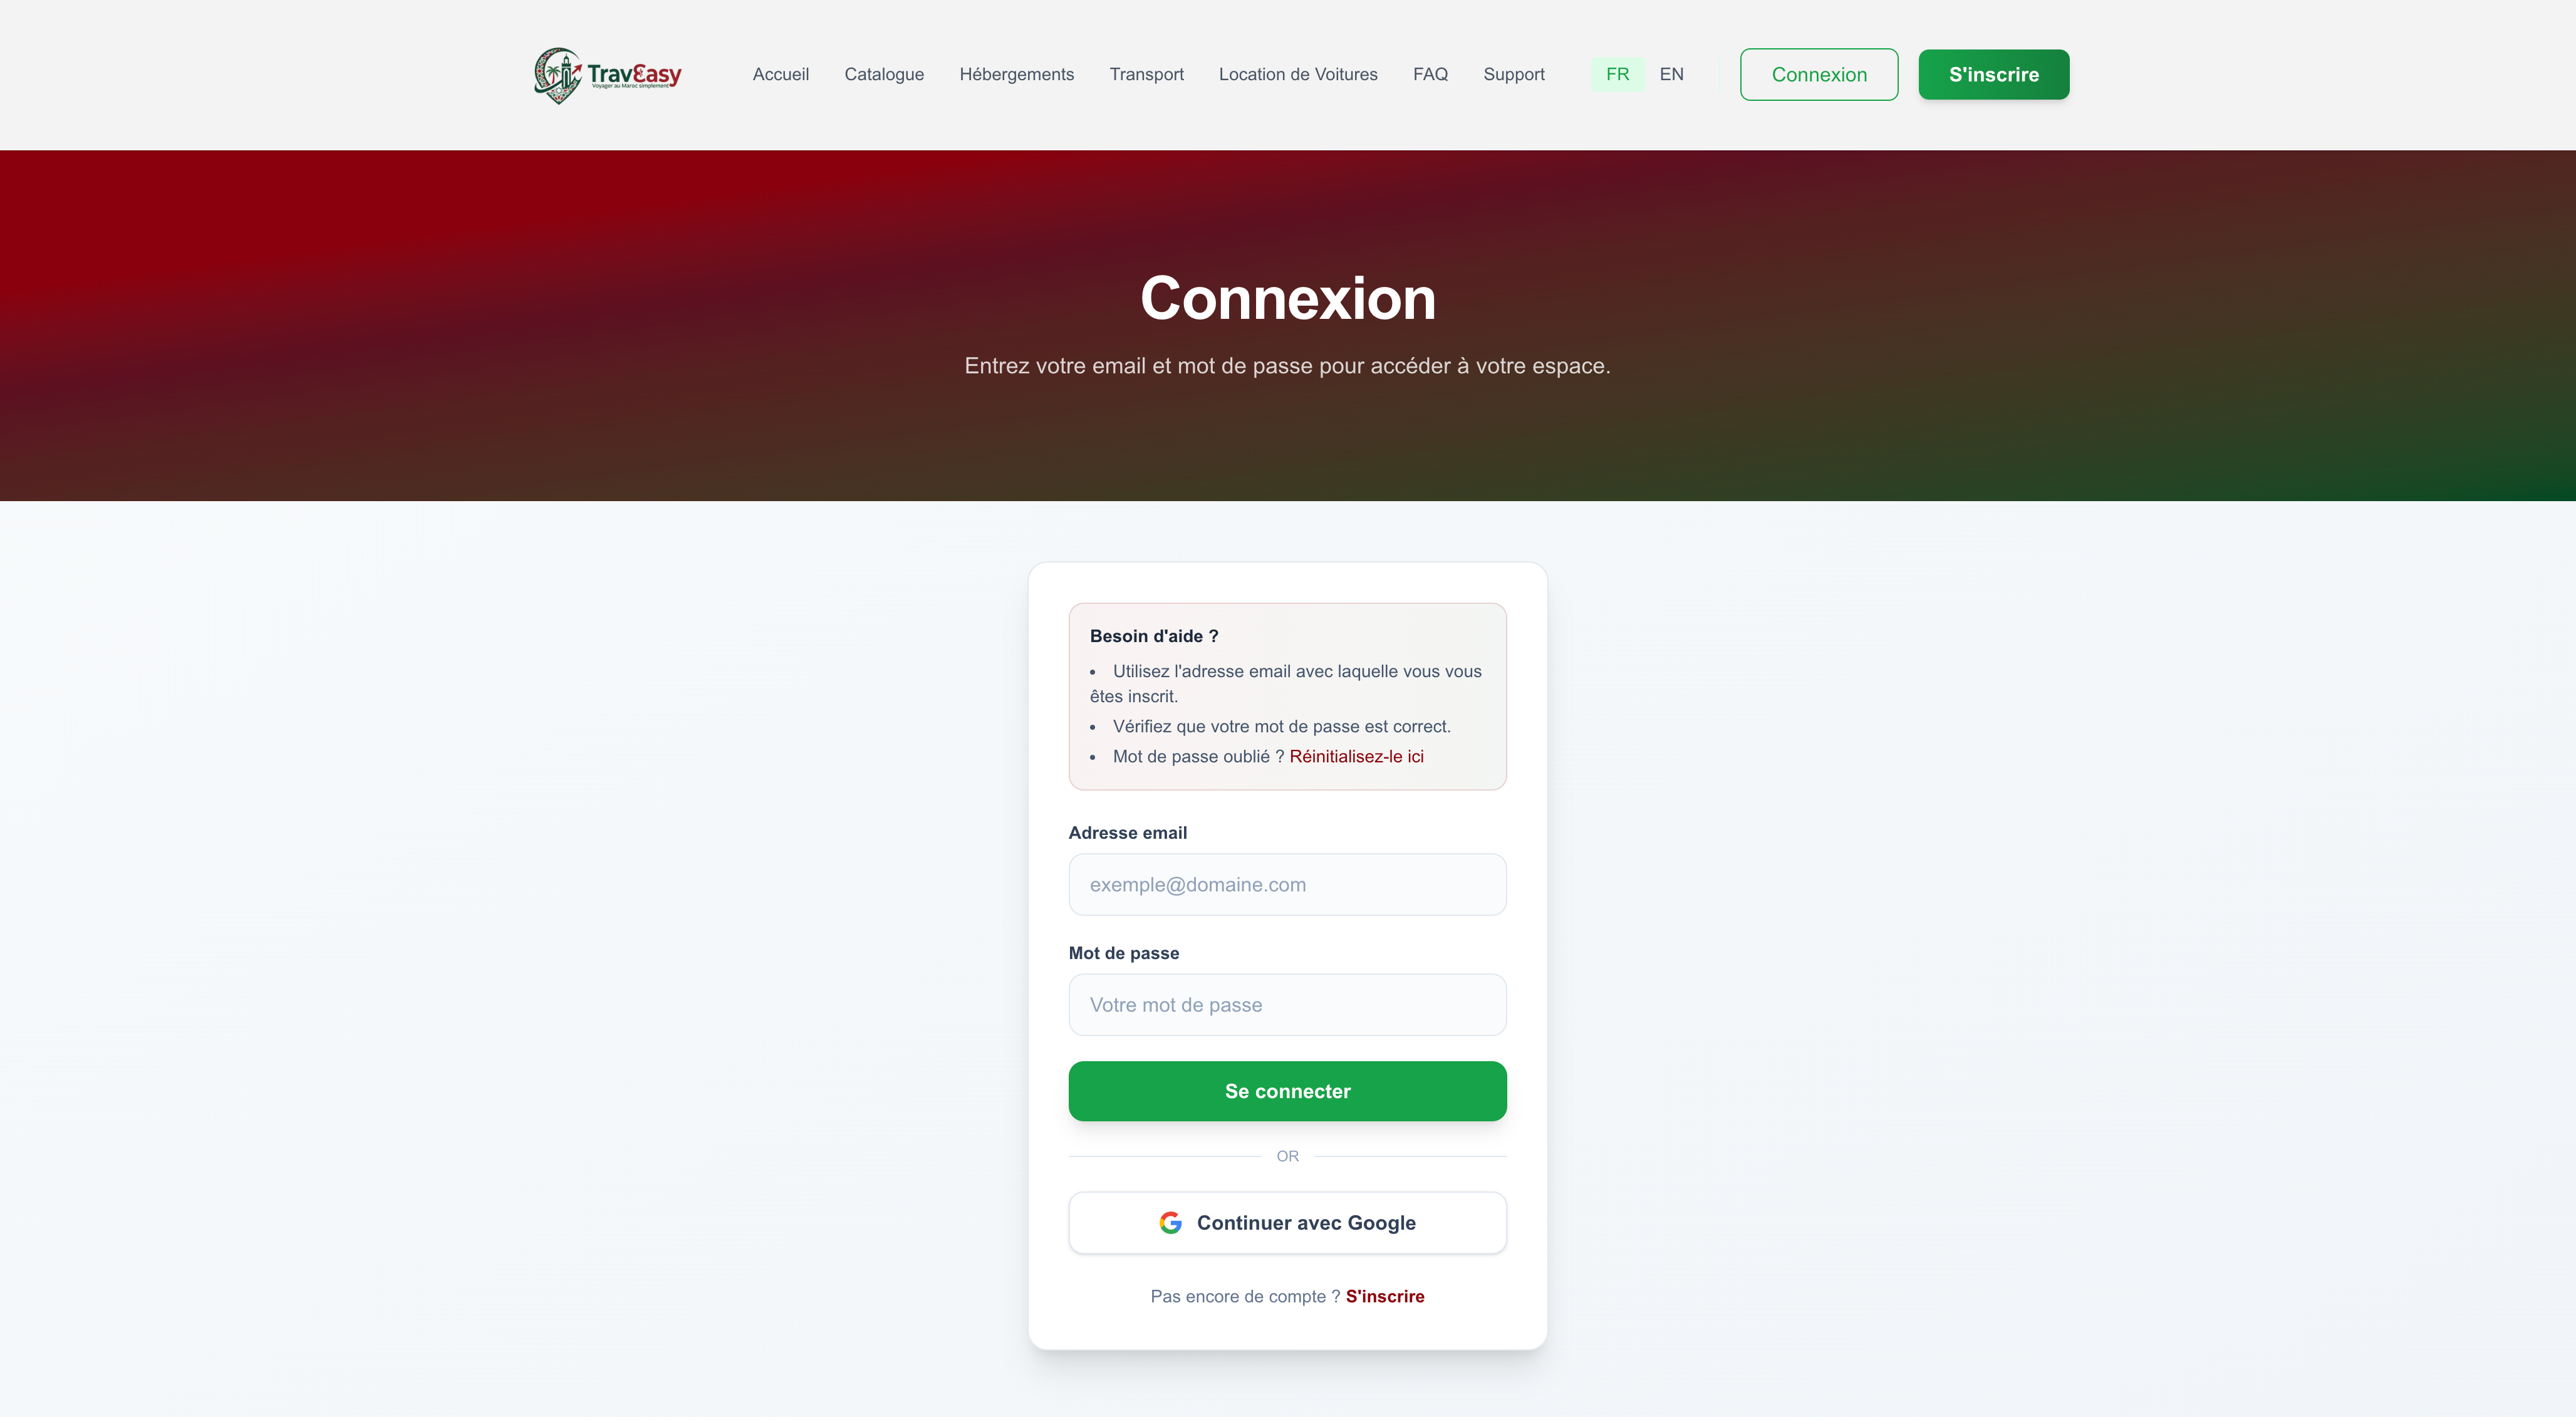
\includegraphics[width=\textwidth]{login.png}
\caption{Formulaire de connexion}
\label{fig:Formulaire de connexion}
\end{figure}

Le formulaire de connexion permet aux utilisateurs enregistrés d'accéder à leur espace personnel. Il repose sur le module Firebase et intègre un mécanisme de gestion des rôles afin de contrôler les niveaux d'accès et les autorisations selon le profil de chaque utilisateur.

\end{spacing}

\subsection{Module de recherche touristique}
\vspace{0.5cm}
\begin{spacing}{1.5}
\justifying
Le module de recherche et de recommandation a été conçu pour faciliter l’accès aux informations touristiques et améliorer l’expérience de navigation des utilisateurs. Il intègre une fonctionnalité de \textbf{recherche multicritère} permettant de trouver rapidement des destinations, activités ou hébergements selon différents paramètres. Afin d’affiner les résultats obtenus, le système propose plusieurs options de \textbf{filtrage} adaptées aux besoins des utilisateurs. Les résultats peuvent également être \textbf{triés par note} afin de mettre en avant les offres les mieux évaluées, ou \textbf{triés par prix} pour faciliter la comparaison des différentes options disponibles. Enfin, une fonctionnalité de \textbf{gestion des favoris} permet aux utilisateurs de sauvegarder les destinations ou services qui les intéressent et de les consulter ultérieurement. Cette approche contribue à rendre la plateforme plus intuitive, personnalisée et efficace.
%Interface de recherche
\begin{figure}[H]
\centering
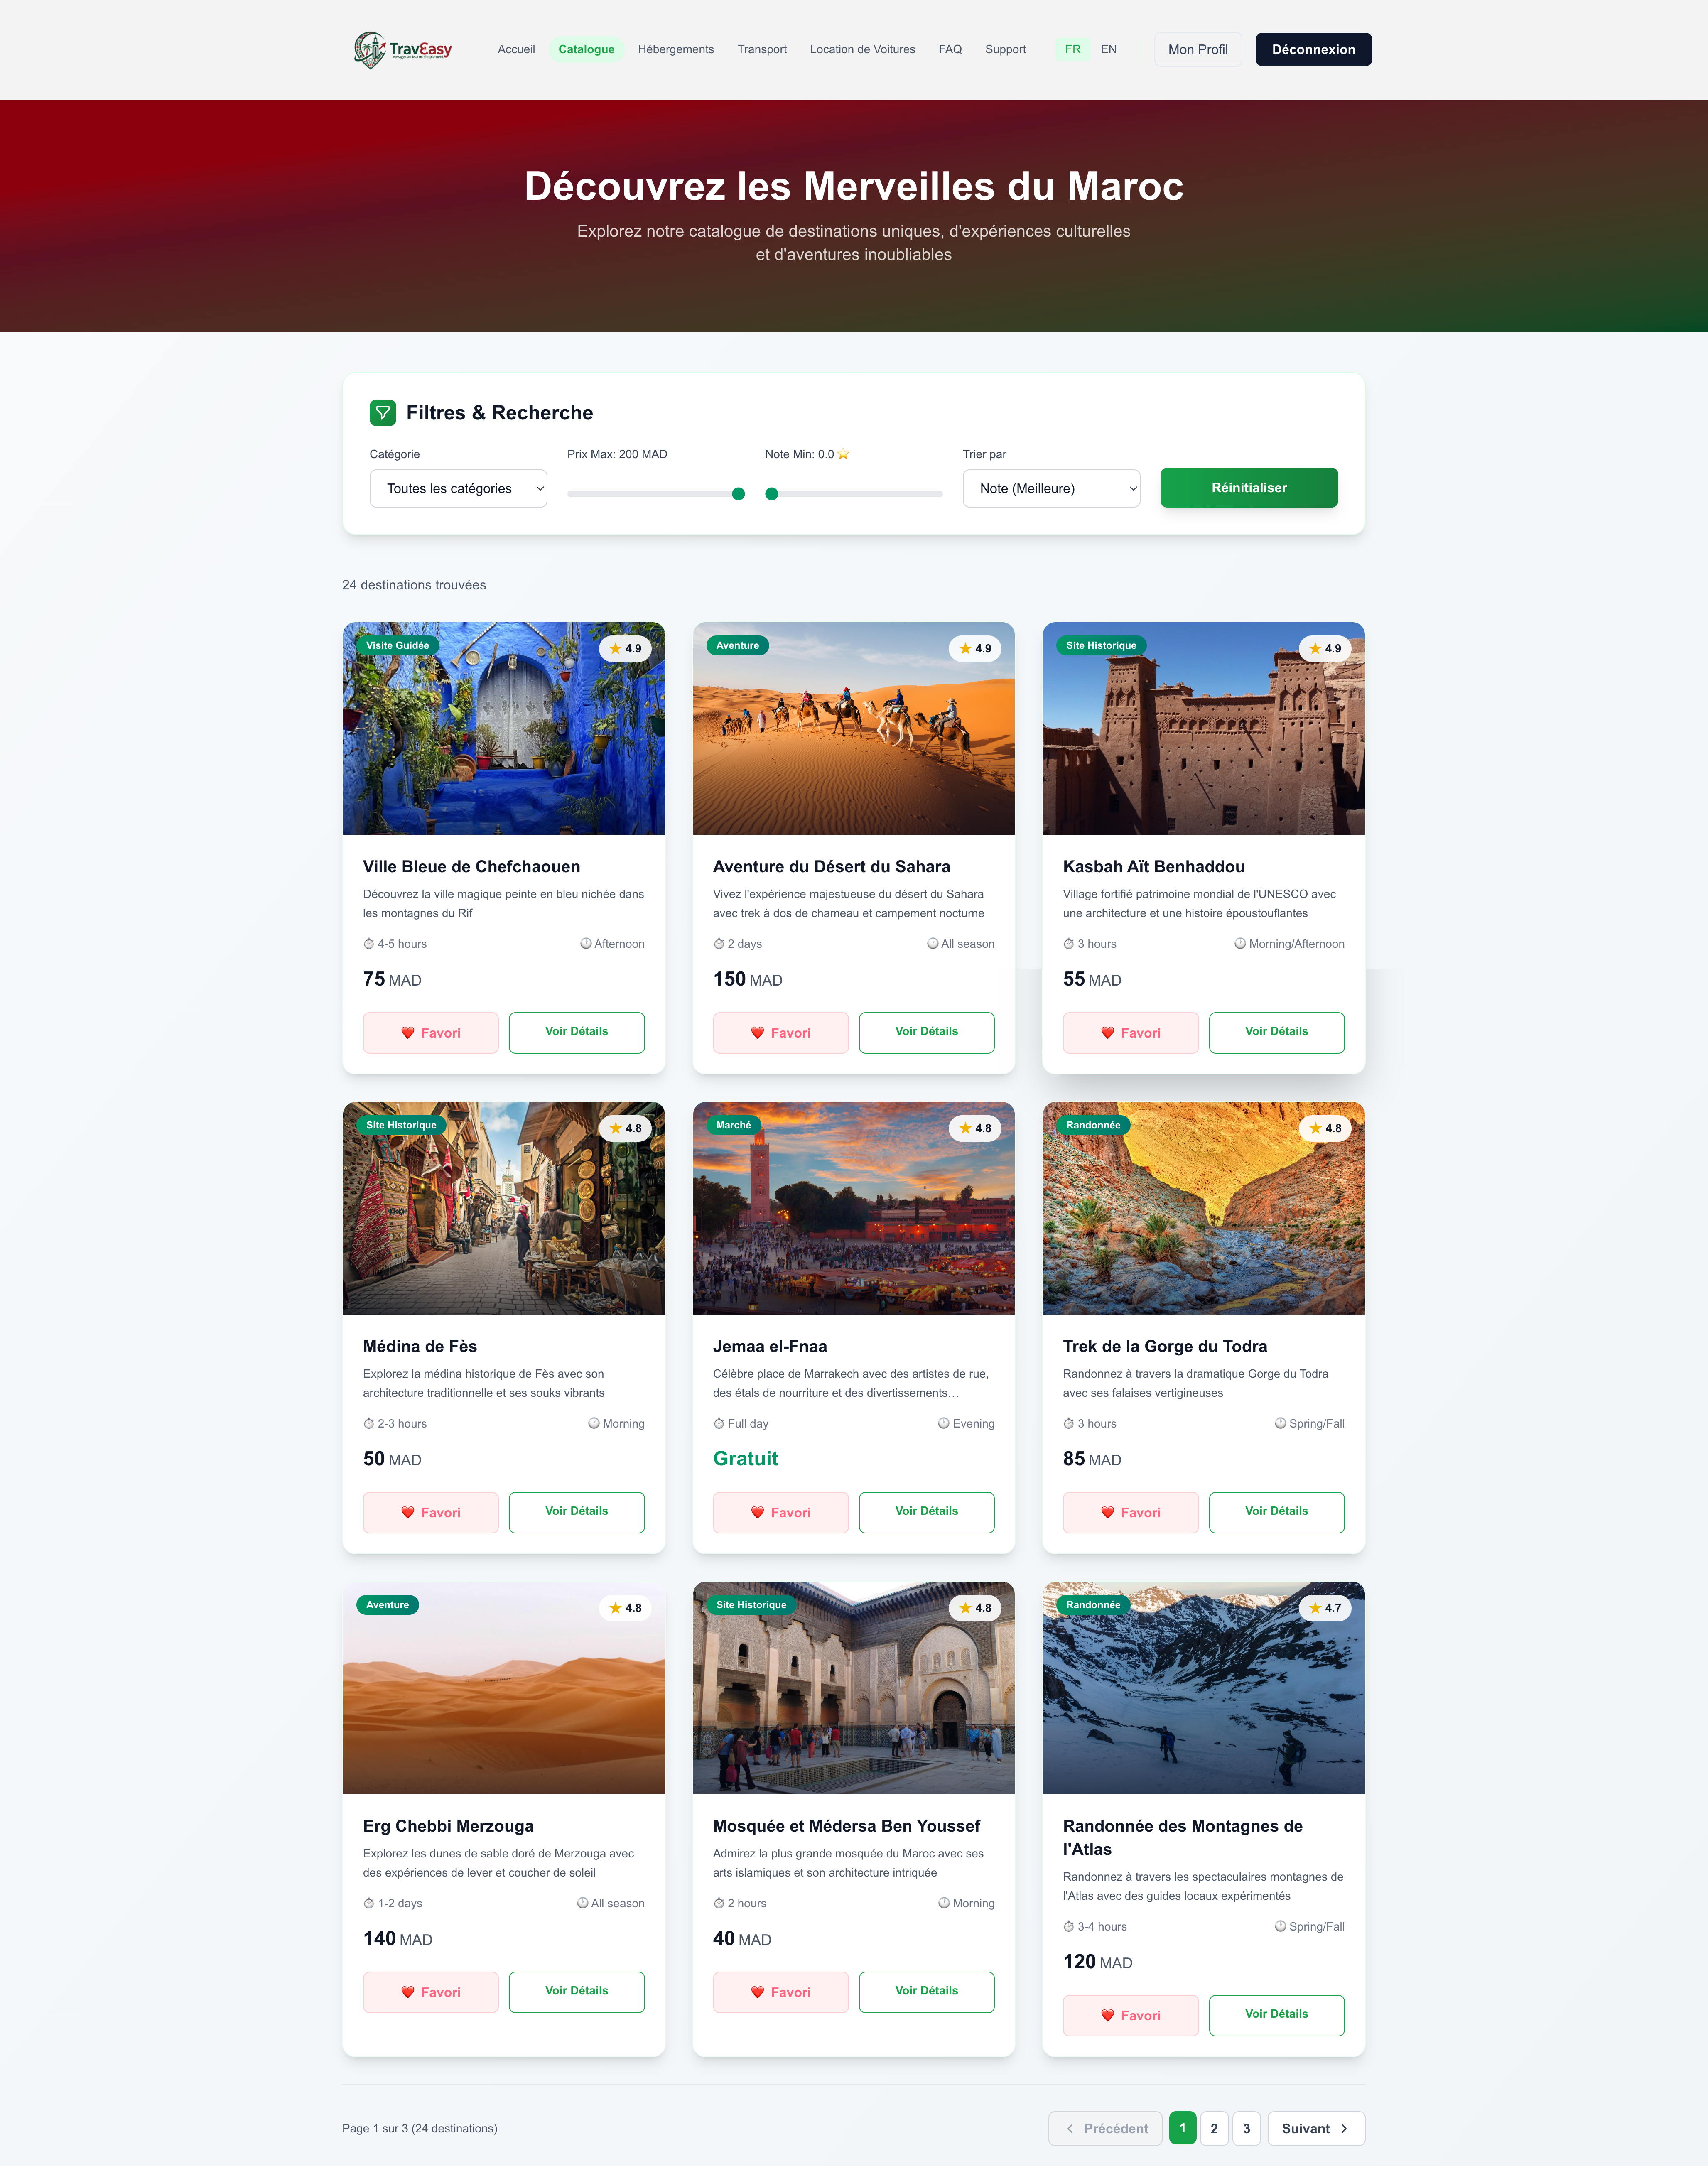
\includegraphics[width=\textwidth]{catalog.png}
\caption{Page du catalogue}
\label{fig:Page du catalogue}
\end{figure}

La page du catalogue présente l'ensemble des destinations et activités touristiques disponibles sur la plateforme. Elle intègre une fonctionnalité de recherche multicritère, des options de filtrage et de tri par note ou par prix, facilitant ainsi la navigation et la découverte des offres.

\begin{figure}[H]
\centering
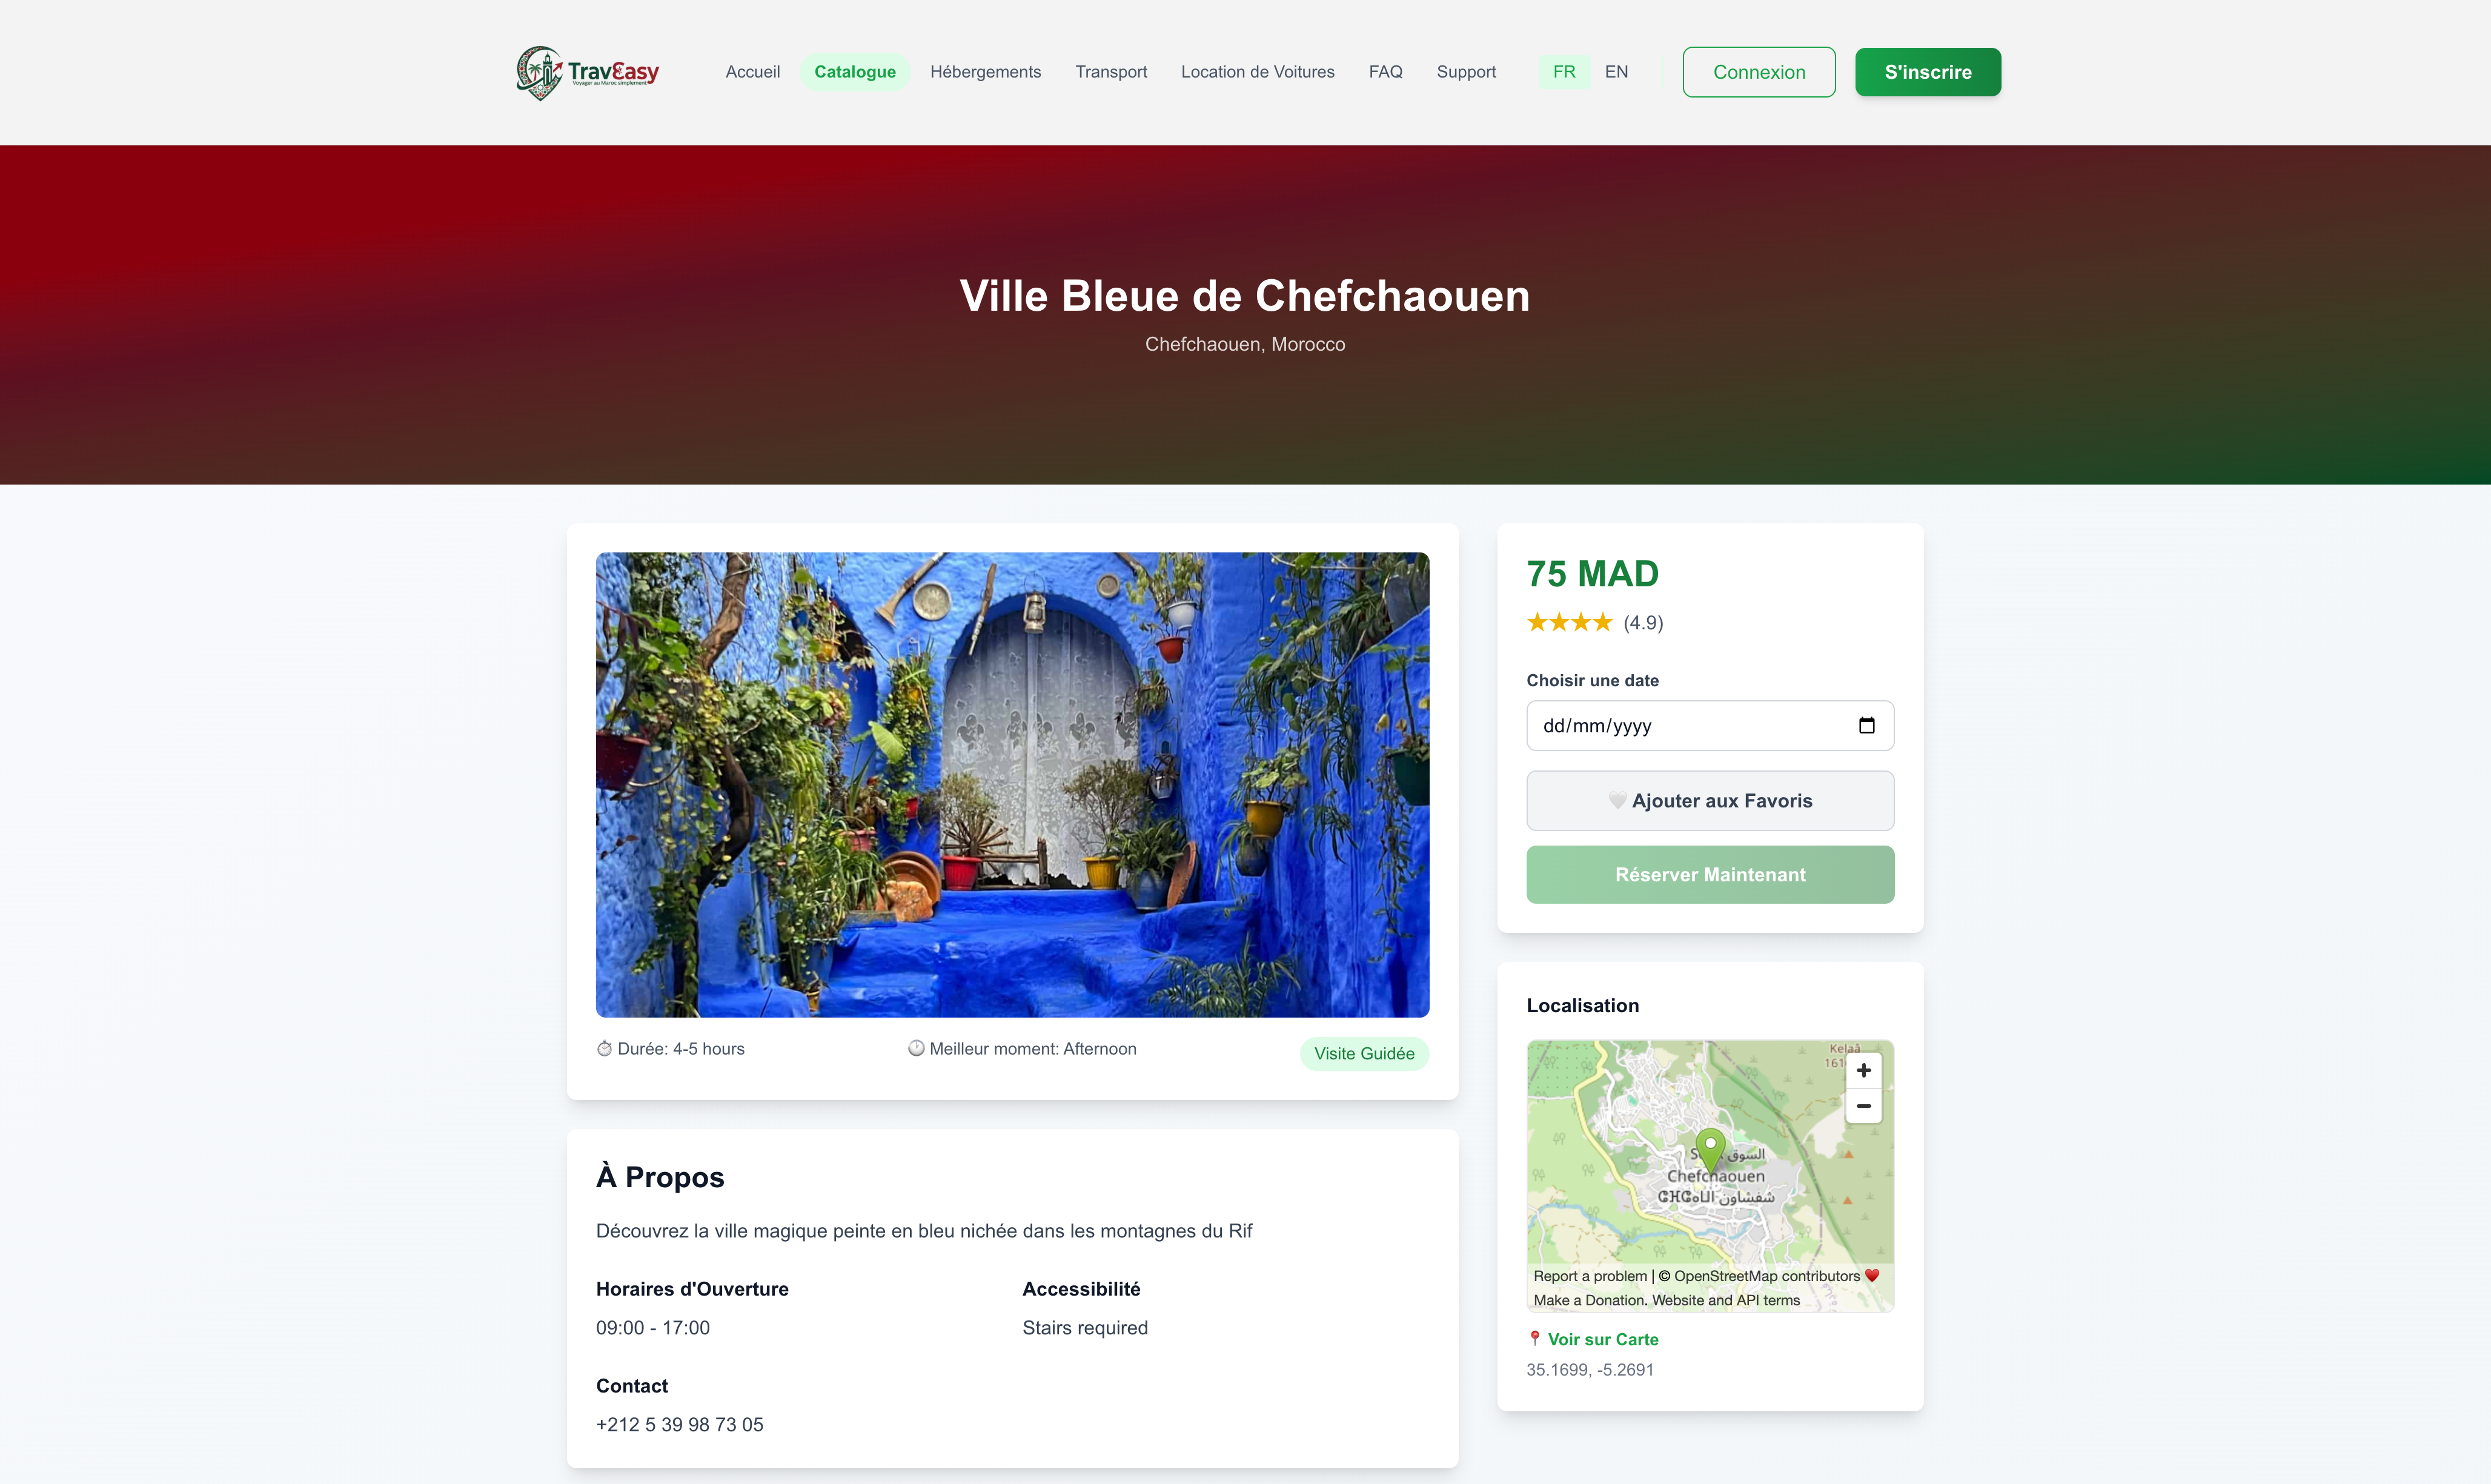
\includegraphics[width=\textwidth]{catalg detail1.png}
\caption{Exemple d'activité à réserver}
\label{fig:Exemple d'activité à réserver}
\end{figure}

Cette figure illustre la fiche détaillée d'une activité touristique disponible à la réservation. L'utilisateur peut y consulter les informations complètes de l'activité et l'ajouter à ses favoris pour la retrouver ultérieurement.

\subsection{Module d’hébergement}
\vspace{0.5cm}
\begin{spacing}{1.5}
\justifying
Le module d’hébergement a été développé afin de permettre aux utilisateurs de rechercher et de consulter différents types d’établissements touristiques disponibles sur la plateforme, notamment les hôtels, les riads, les auberges et les maisons d’hôtes. Ce module vise à faciliter l’accès aux informations relatives aux hébergements et à aider les utilisateurs dans le choix d’un établissement adapté à leurs besoins et à leur budget.

Parmi les principales fonctionnalités proposées figurent la consultation des hébergements disponibles, la recherche par nom ou par ville, ainsi que plusieurs options de filtrage permettant d’affiner les résultats selon différents critères tels que le type d’hébergement, la ville, le nombre d’étoiles ou encore la gamme de prix. Afin d’améliorer l’expérience utilisateur et de faciliter la navigation, les résultats sont organisés à l’aide d’un système de pagination. Le module offre également la possibilité de consulter les détails complets d’un établissement, incluant ses caractéristiques principales et les informations utiles à la réservation. Enfin, une fonctionnalité de redirection vers le site officiel de réservation permet à l’utilisateur d’accéder directement à la plateforme de réservation de l’établissement sélectionné. Cette approche contribue à rendre la recherche d’hébergement plus simple, rapide et efficace.

\begin{figure}[H]
\centering
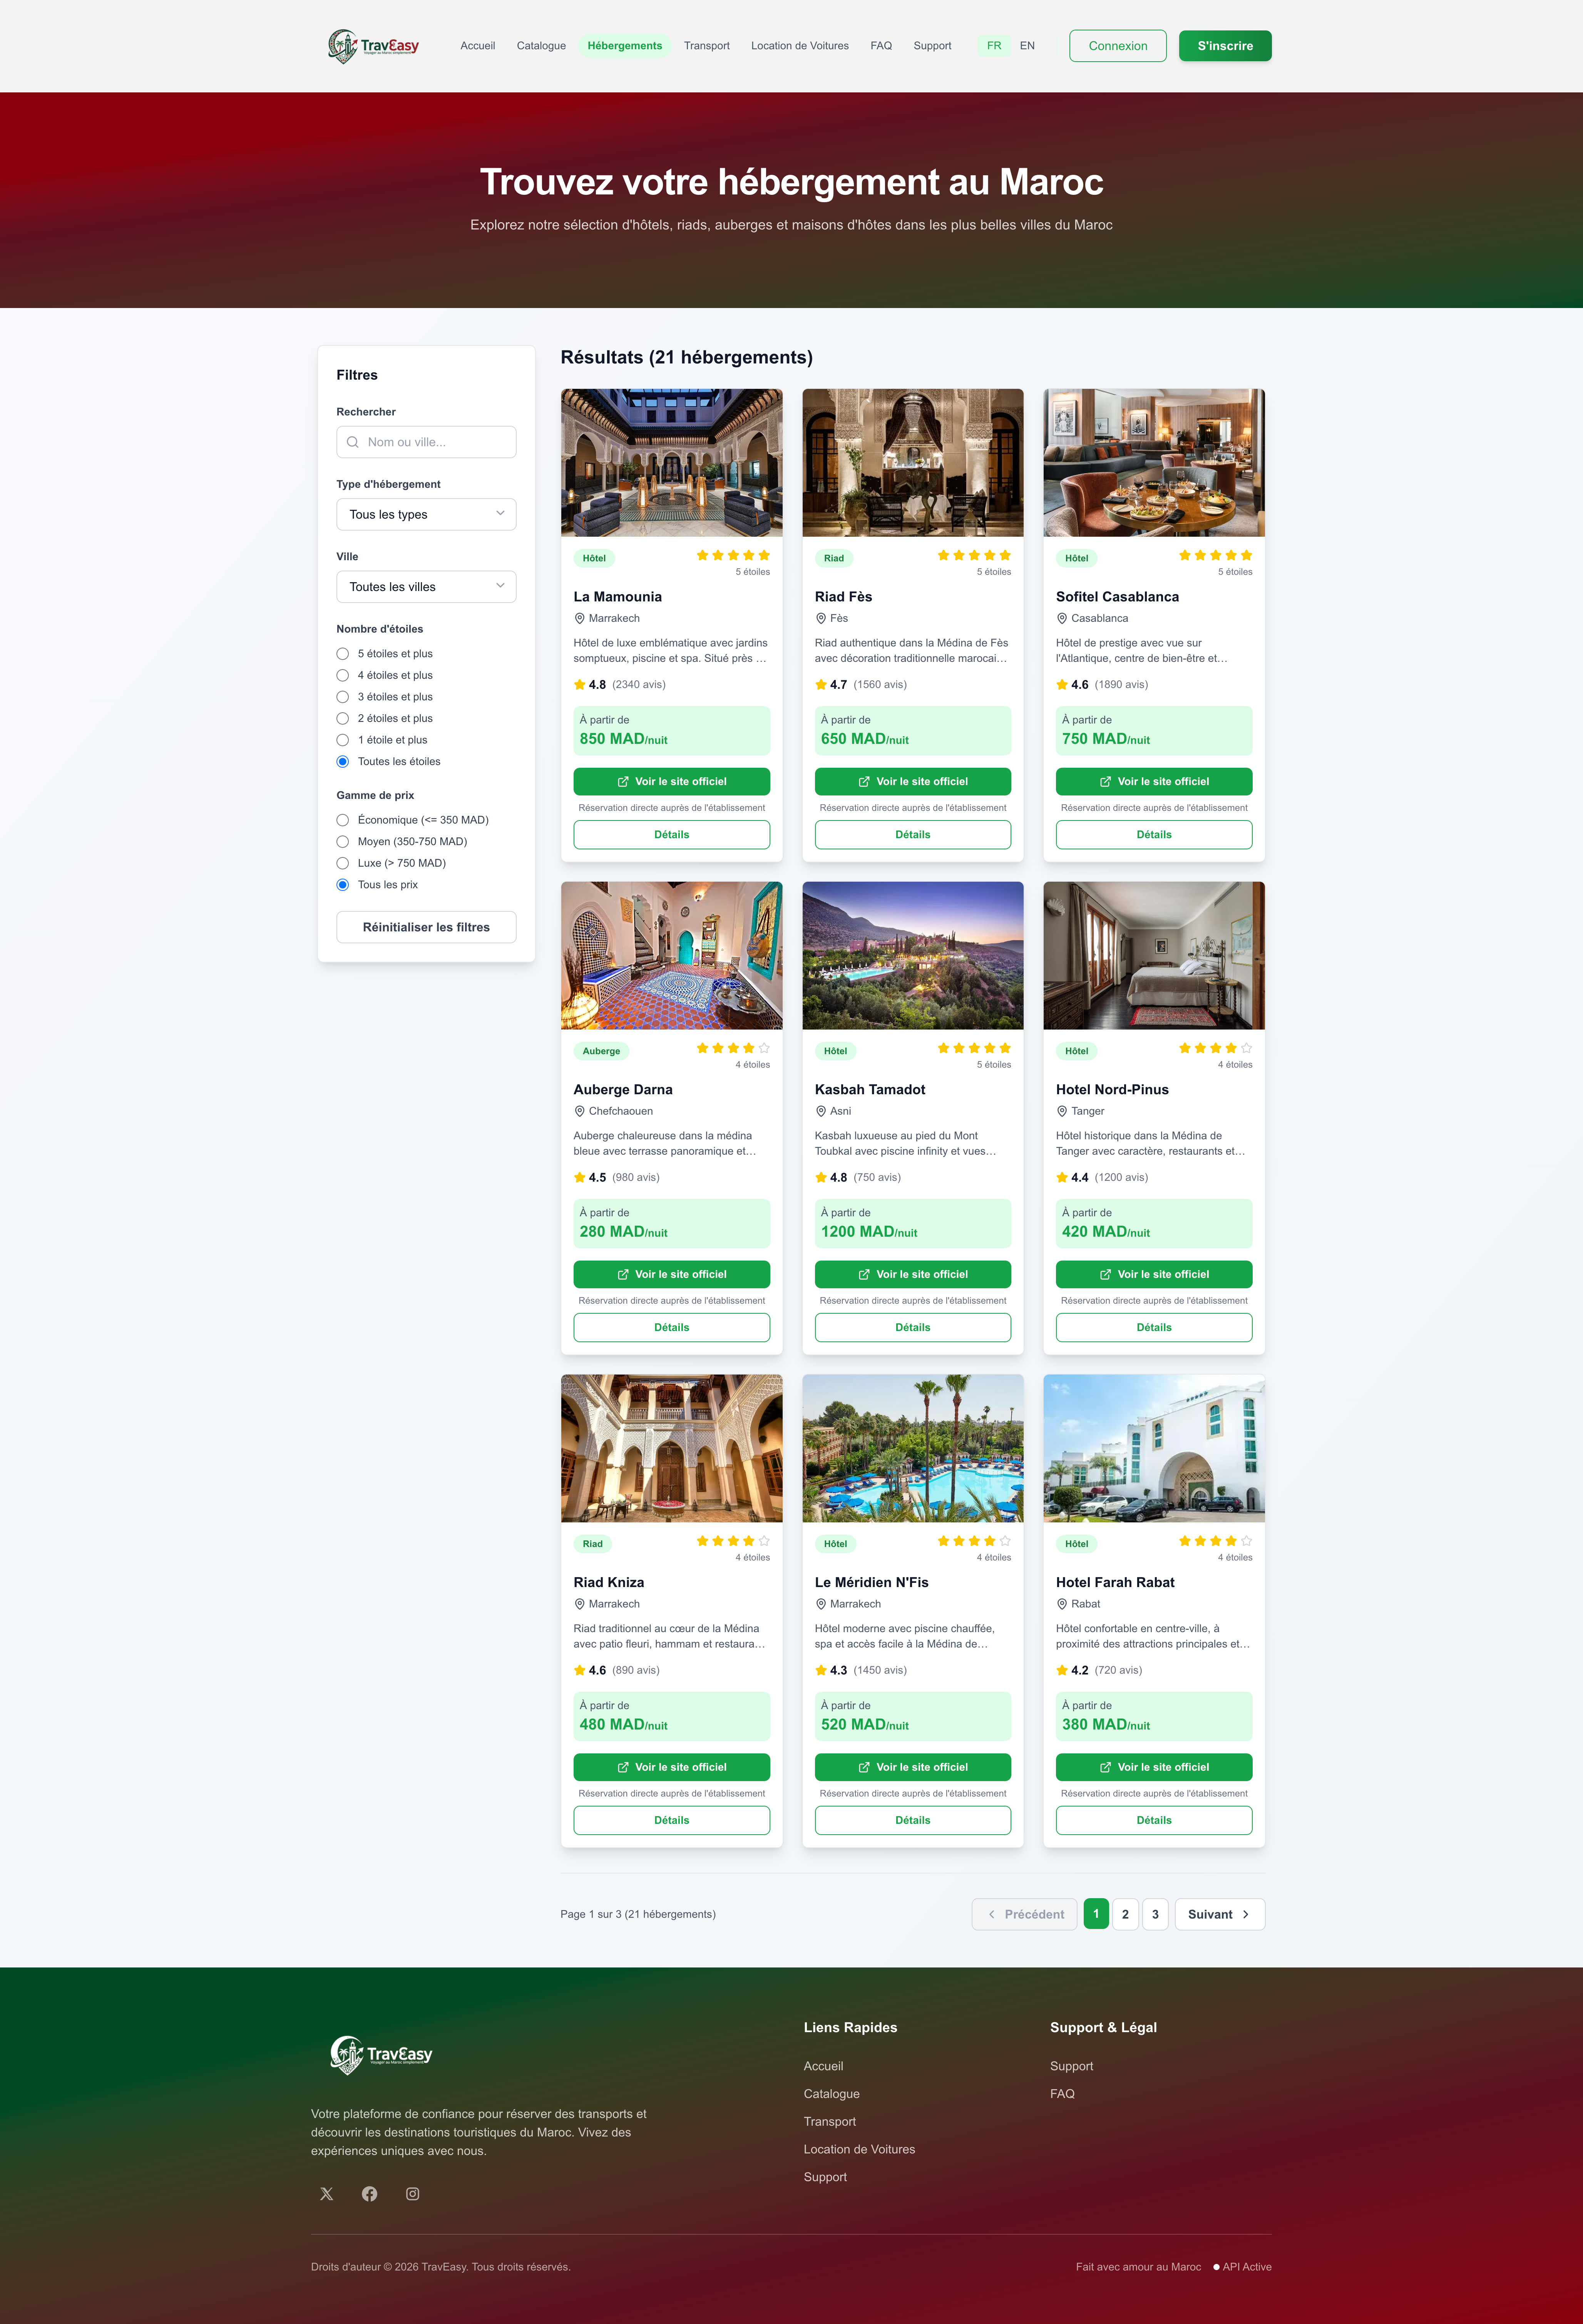
\includegraphics[width=\textwidth]{hebergement.png}
\caption{Page de recherche d'hébergement}
\label{fig:Page de recherche d'hébergement}
\end{figure}

La page de recherche d'hébergement permet aux utilisateurs de consulter les différents types d'établissements disponibles (hôtels, riads, auberges, maisons d'hôtes). Elle propose des options de filtrage par ville, type d'hébergement, nombre d'étoiles et gamme de prix, avec une organisation paginée des résultats.

\begin{figure}[H]
\centering
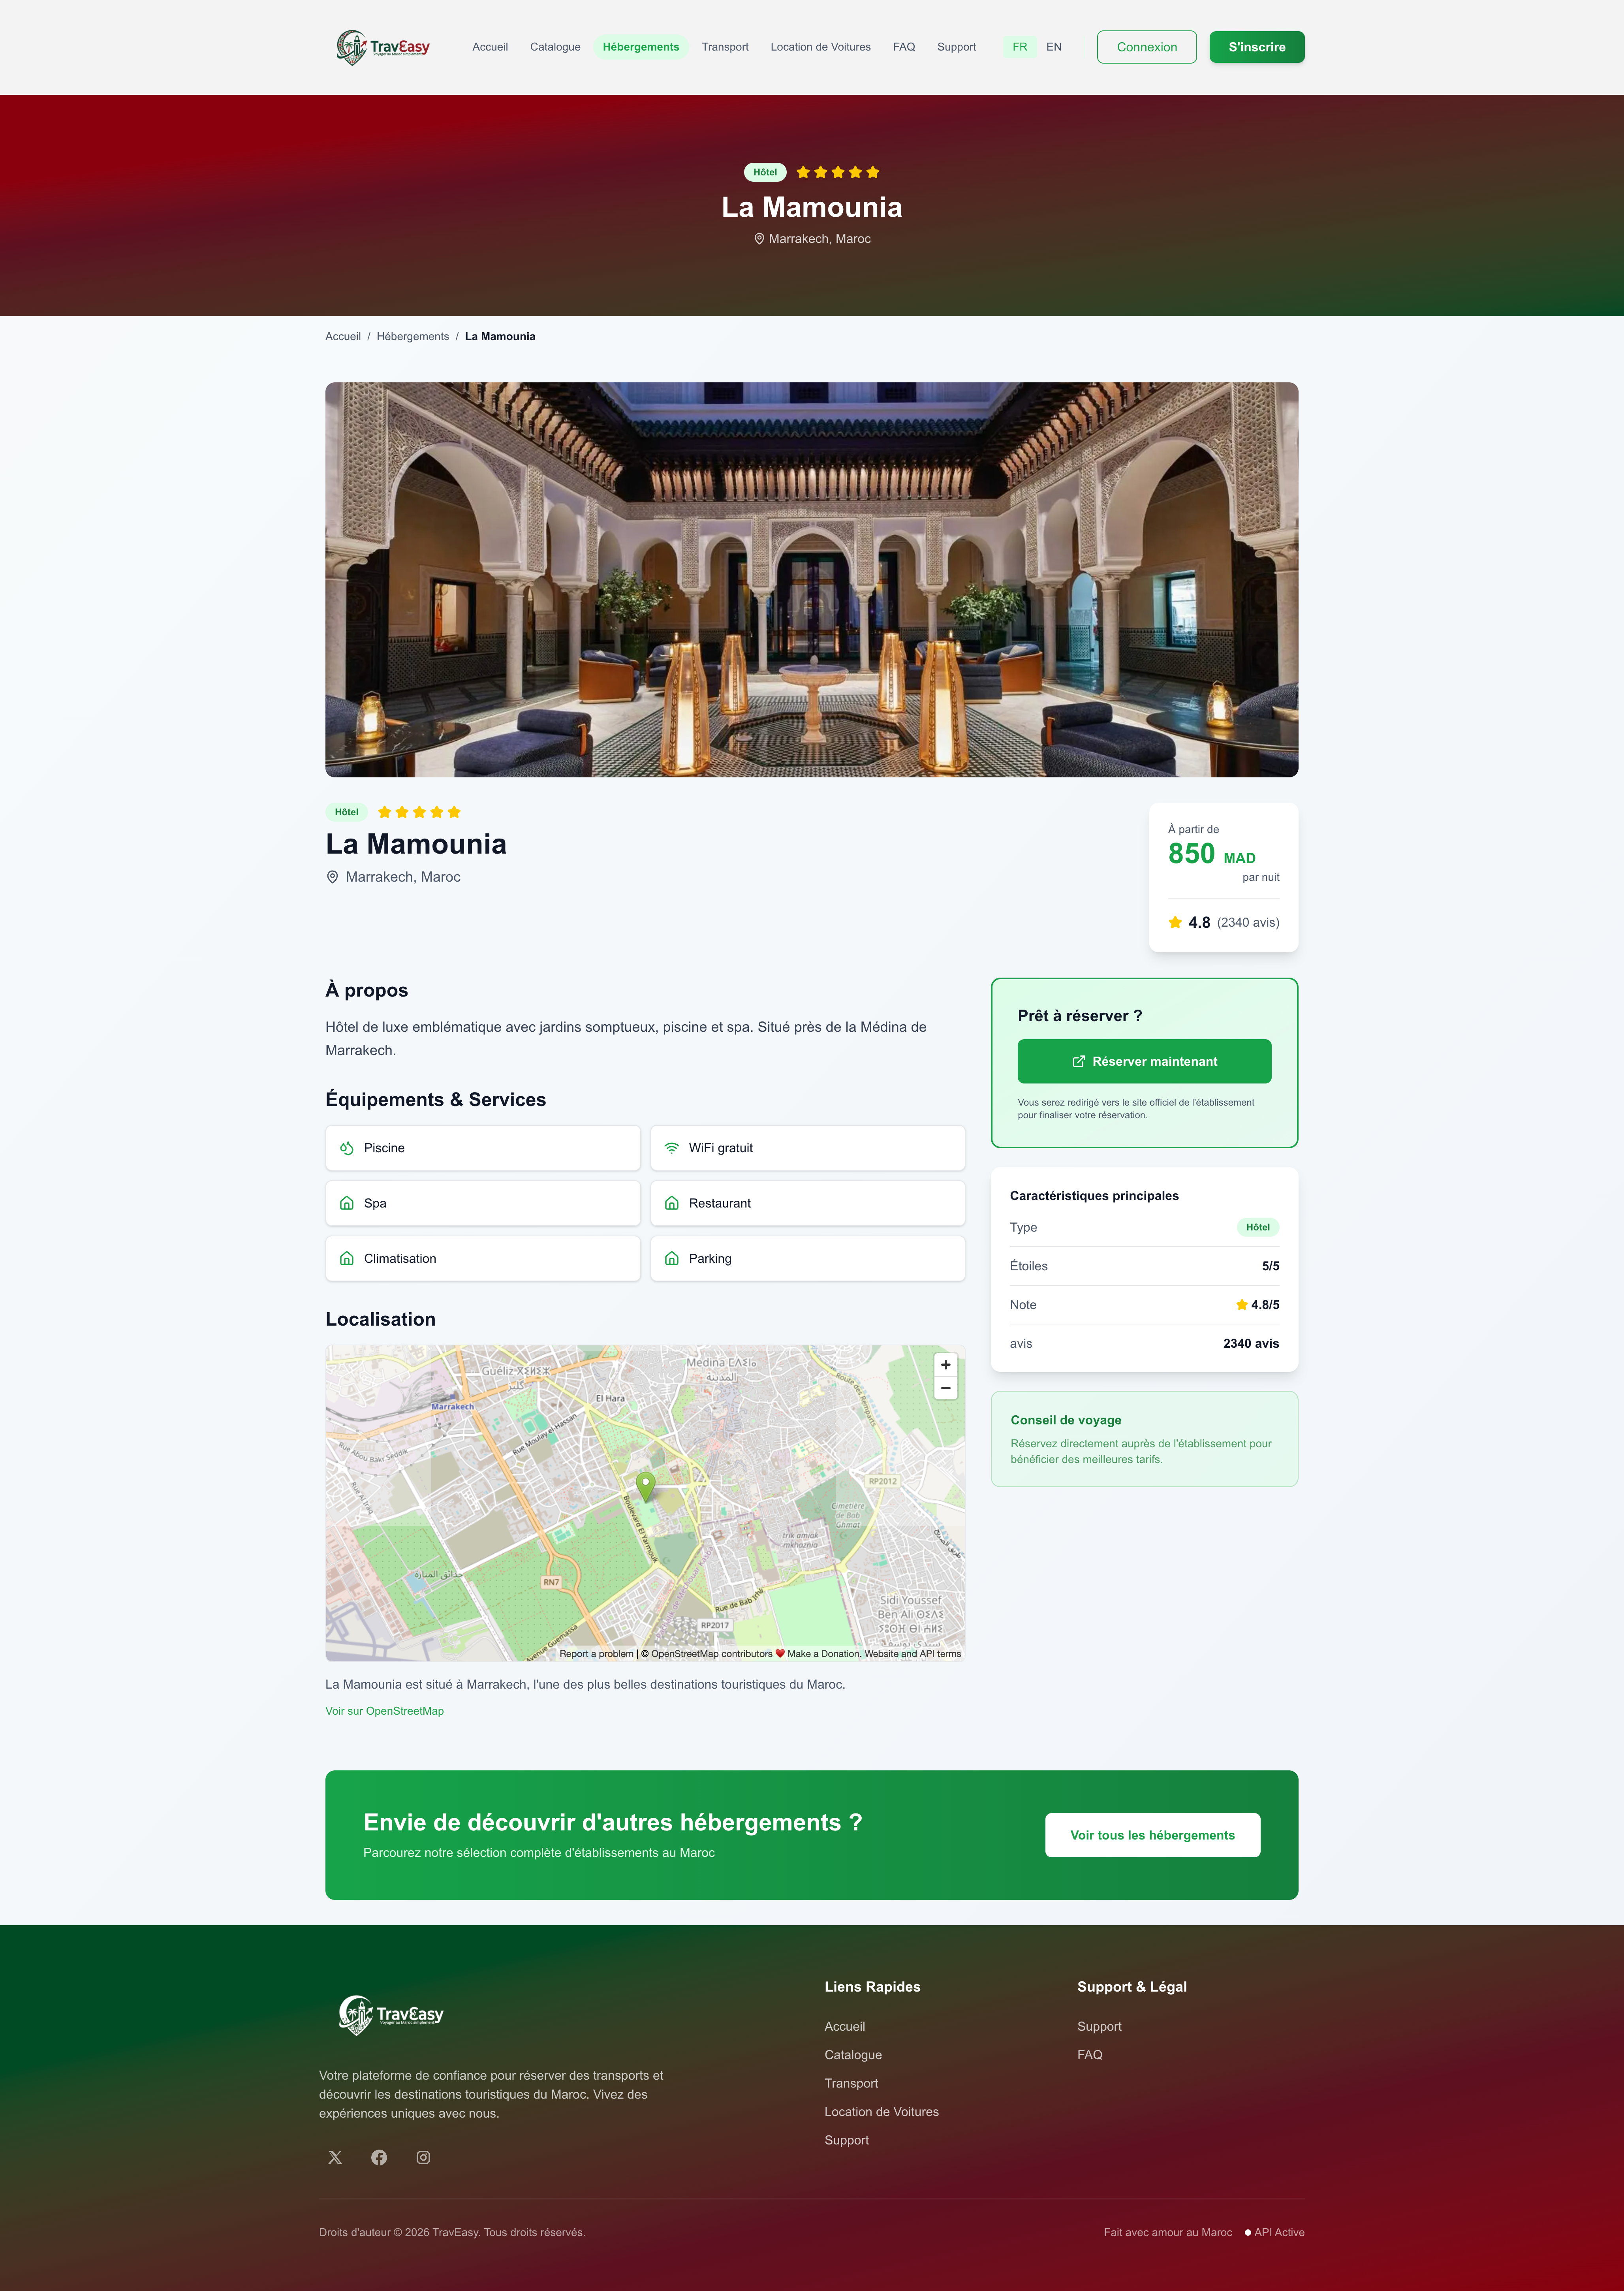
\includegraphics[width=\textwidth]{hotel.png}
\caption{Exemple d'hébergement}
\label{fig:Exemple d'hébergement}
\end{figure}

Cette figure présente la fiche détaillée d'un hébergement, incluant ses caractéristiques principales, les informations utiles à la réservation ainsi qu'un lien de redirection vers le site officiel de l'établissement.

\end{spacing}
%Interface principale du module d'hébergement.
%Système de recherche et de filtrage des hébergements.
%Affichage paginé des hébergements(chi example dyal chi hotel kiach kitl3)


\end{spacing}



\subsection{Module de réservation de transport}
\vspace{0.5cm}
\begin{spacing}{1.5}
\justifying
Le module de réservation de transport permet aux utilisateurs de réserver facilement un moyen de transport pour leurs déplacements. 
Lors du processus de réservation, l’utilisateur sélectionne d’abord son \textbf{point de départ} ainsi que sa \textbf{destination}. 
À partir de ces informations, le système effectue un \textbf{calcul automatique du tarif} en tenant compte de plusieurs paramètres liés au trajet. Une fois le montant calculé et les informations vérifiées, l’utilisateur peut procéder à la \textbf{confirmation de la réservation}.
Le calcul du prix est basé sur une formule tarifaire permettant d’adapter le coût du trajet aux différentes conditions de transport. Cette formule est définie comme suit :
\begin{equation}
\begin{aligned}
\text{Prix} = {}& \text{TarifBase} + (\text{Distance} \times \text{Coefficient}) \\
& + \text{MajorationNuit} + \text{MajorationWeekend} + \text{MajorationSaison}
\end{aligned}
\end{equation}
où :
\begin{itemize}
    \item \textbf{TarifBase} représente le coût fixe appliqué à chaque réservation ;
    \item \textbf{Distance} correspond à la distance parcourue entre le point de départ et la destination ;
    \item \textbf{Coefficient} désigne le coût appliqué par kilomètre parcouru ;
    \item \textbf{MajorationNuit} est un supplément appliqué aux trajets effectués pendant les horaires nocturnes ;
    \item \textbf{MajorationWeekend} correspond à un ajustement tarifaire appliqué durant les week-ends ;
    \item \textbf{MajorationSaison} représente une majoration liée aux périodes de forte affluence touristique.
\end{itemize}
Cette méthode de calcul permet d’obtenir une tarification dynamique, équitable et adaptée aux différentes conditions d’exploitation du service de transport. 
Pour l’utilisateur, le montant est affiché de manière transparente avant la validation définitive de la réservation.

%Capture écran transpot
\begin{figure}[H]
\centering
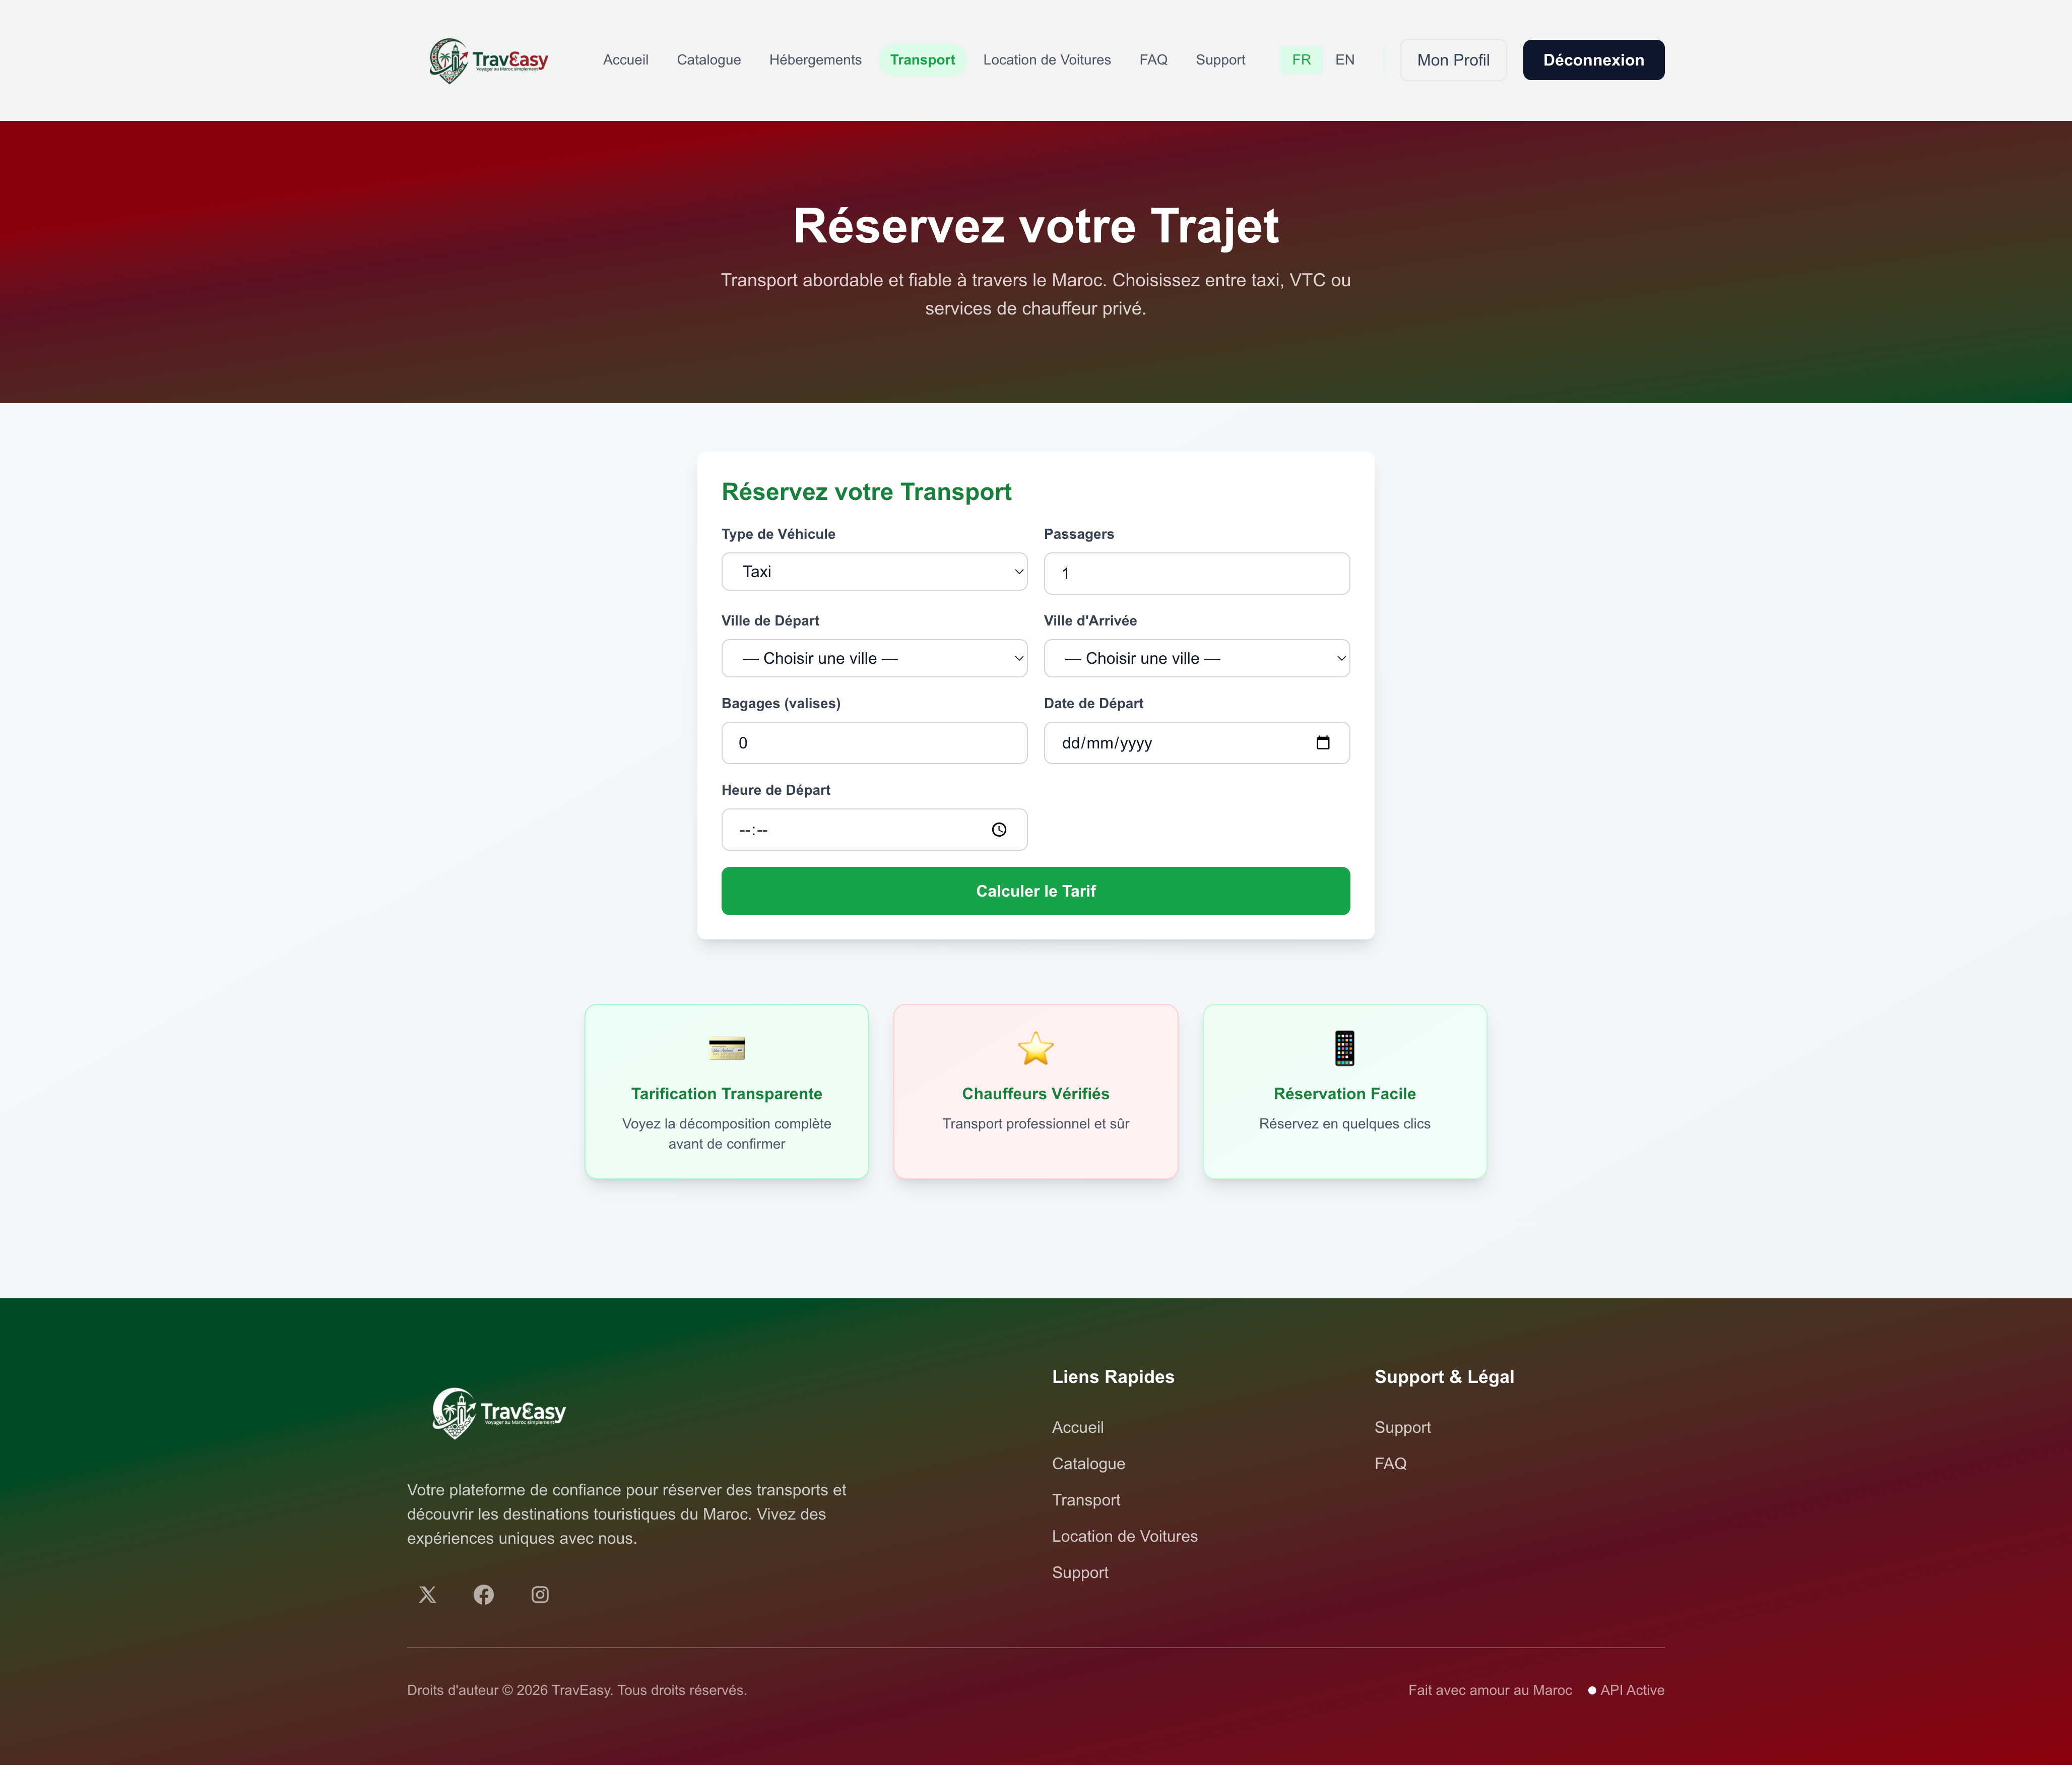
\includegraphics[width=\textwidth]{transport.png}
\caption{Page de transport}
\label{fig:Page de transport}
\end{figure}


La page de transport permet à l'utilisateur de saisir son point de départ et sa destination afin d'initier une réservation. Le système calcule automatiquement le tarif en tenant compte de la distance, du coefficient kilométrique et des majorations applicables (nuit, week-end, saison).

%Capture écran estimation du prix
\begin{figure}[H]
\centering
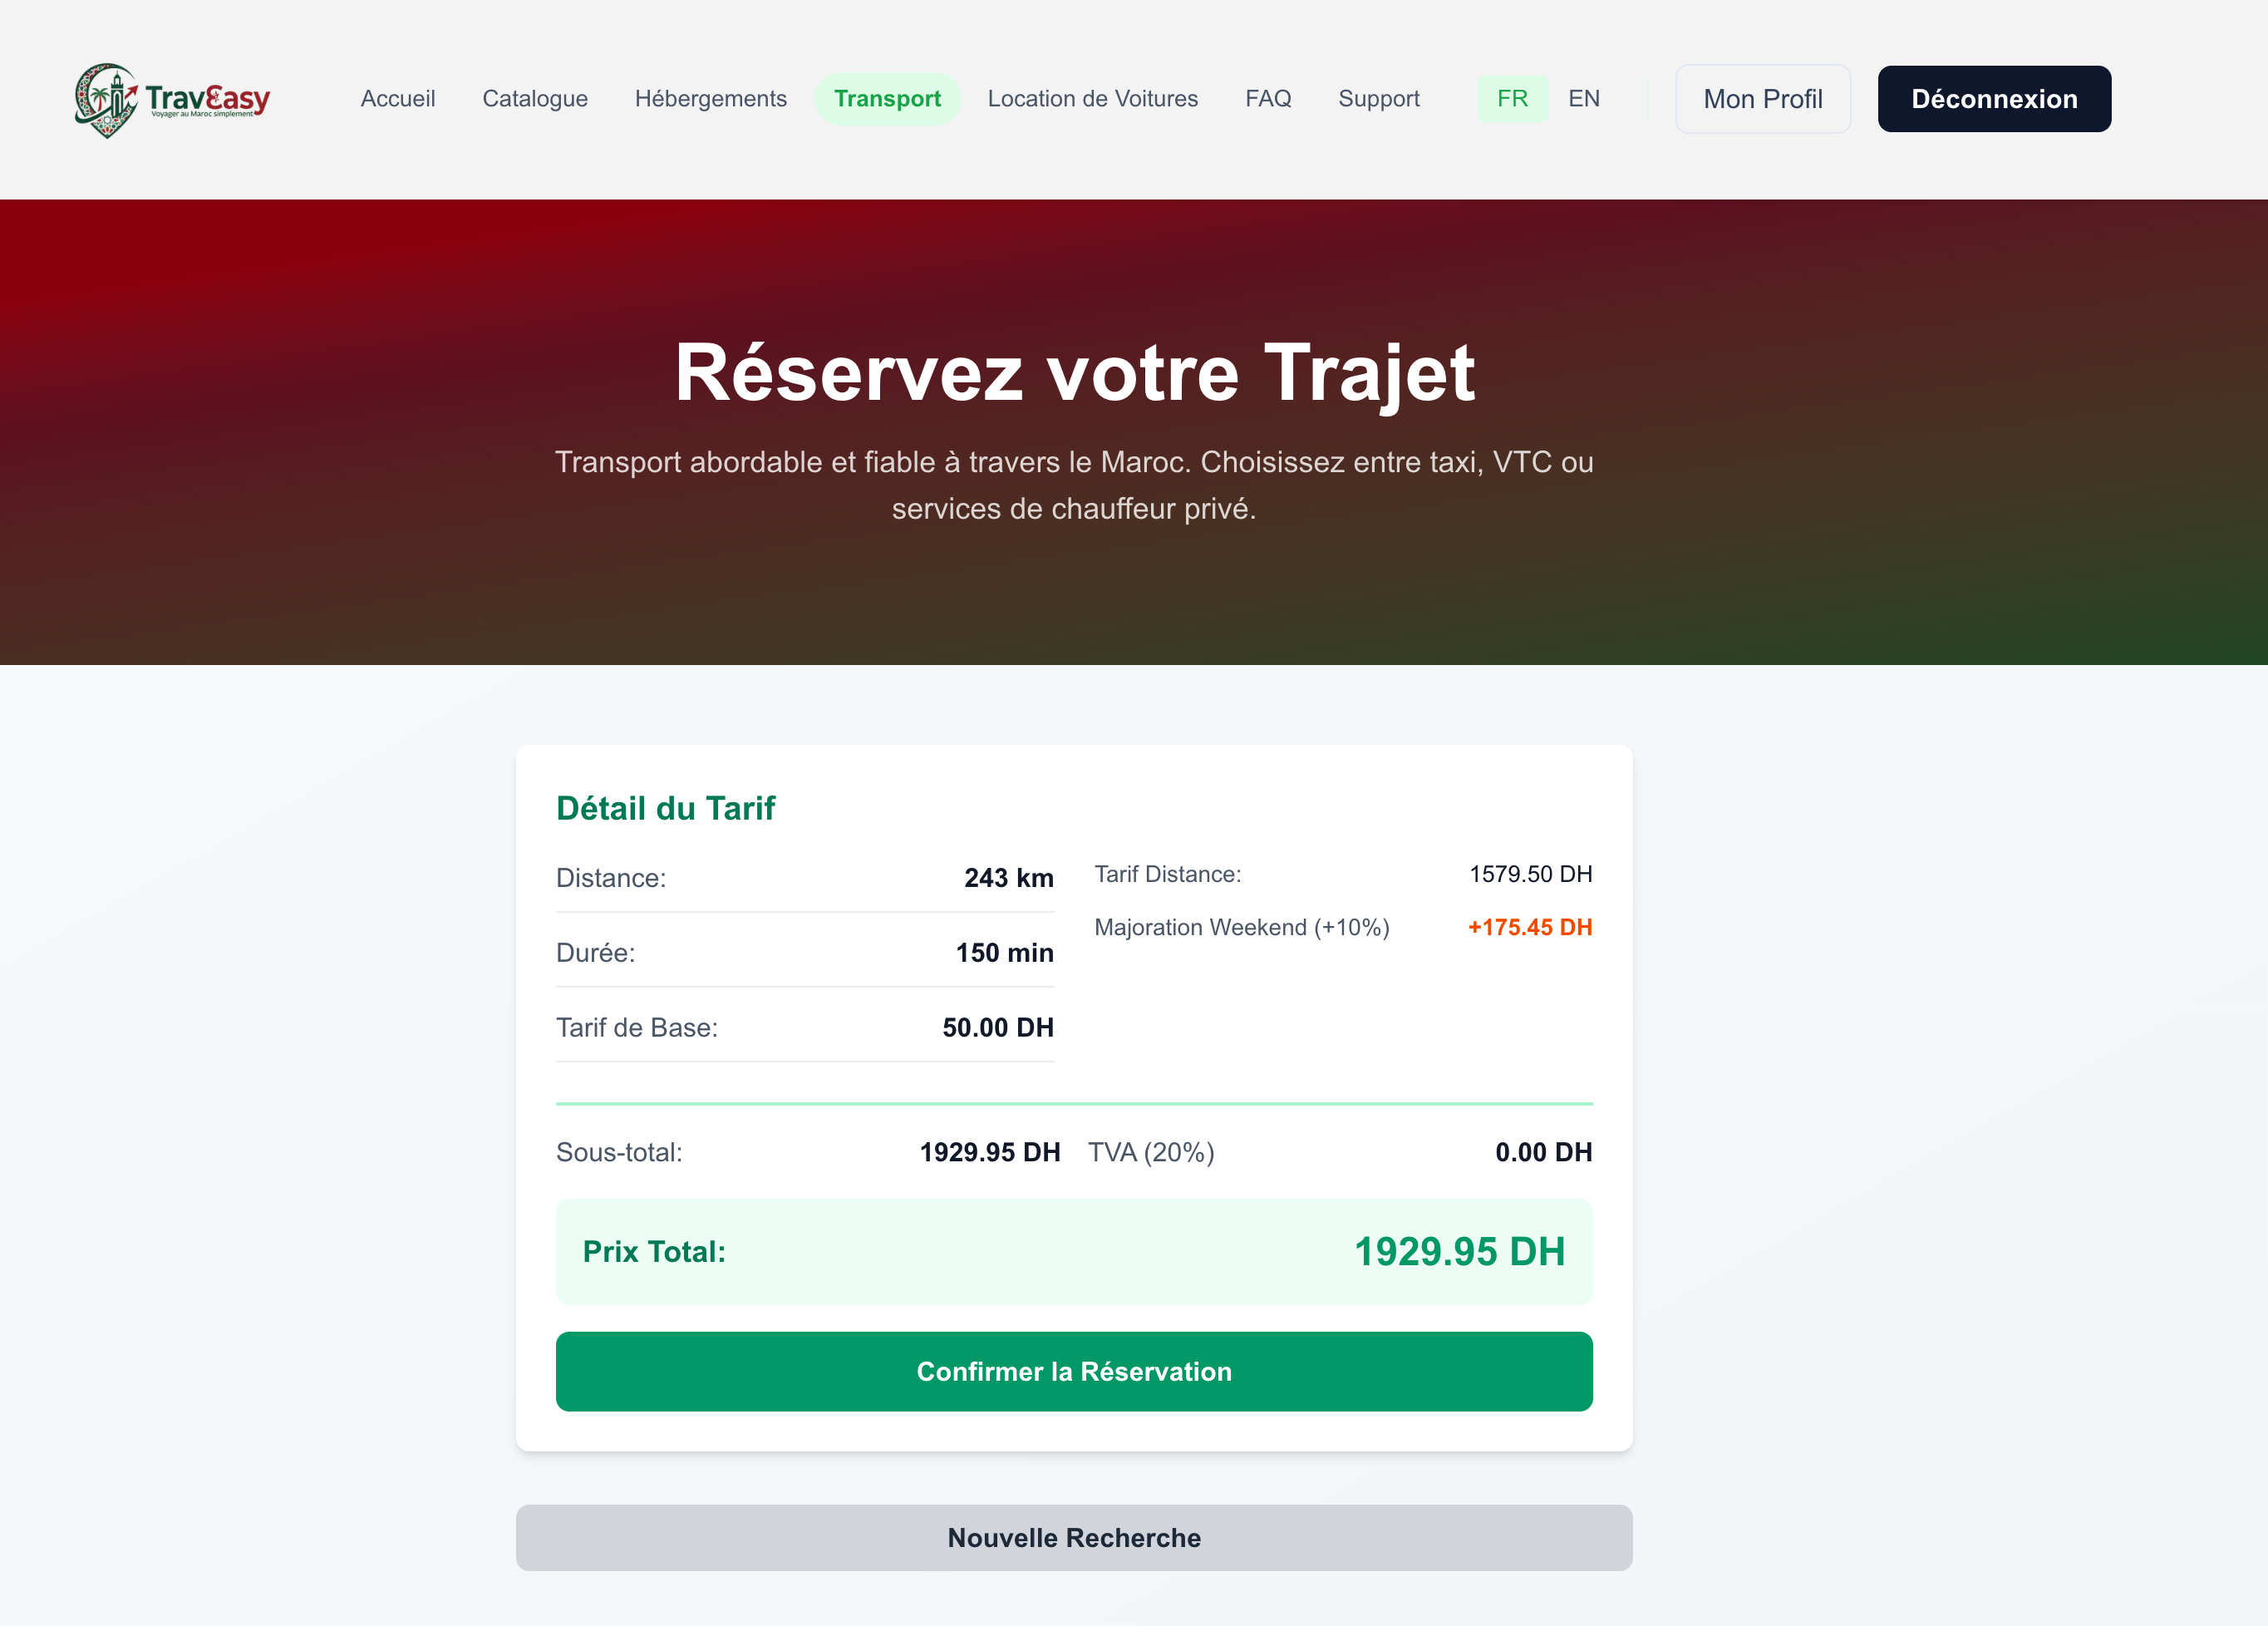
\includegraphics[width=\textwidth]{transport detail.png}
\caption{Exemple de détail de transport}
\label{fig:Exemple de détail de transport}
\end{figure}


Cette figure illustre la vue détaillée d'une réservation de transport, affichant de manière transparente le montant calculé selon la formule tarifaire dynamique avant la validation définitive par l'utilisateur.

\subsection{Module de Location de voiture}
\vspace{0.5cm}
\begin{spacing}{1.5}
\justifying
Le module de location de voiture permet aux utilisateurs de réserver des véhicules directement depuis la plateforme. Après avoir sélectionné un véhicule, l’utilisateur peut consulter les détails du véhicule, 
vérifier sa disponibilité et effectuer une réservation en ligne. 
Le système offre également la possibilité de \textbf{filtrer les véhicules} en fonction de critères spécifiques tels que le type de véhicule, le prix ou les options disponibles. 
Afin de garantir une expérience utilisateur optimale, la plateforme effectue automatiquement le \textbf{calcul du coût total} de la location en fonction de la durée et des options choisies. 
Ce module favorise la transparence, renforce la confiance des utilisateurs et contribue à améliorer la qualité des services proposés.

%Interface de location de voiture
\begin{figure}[H]
\centering
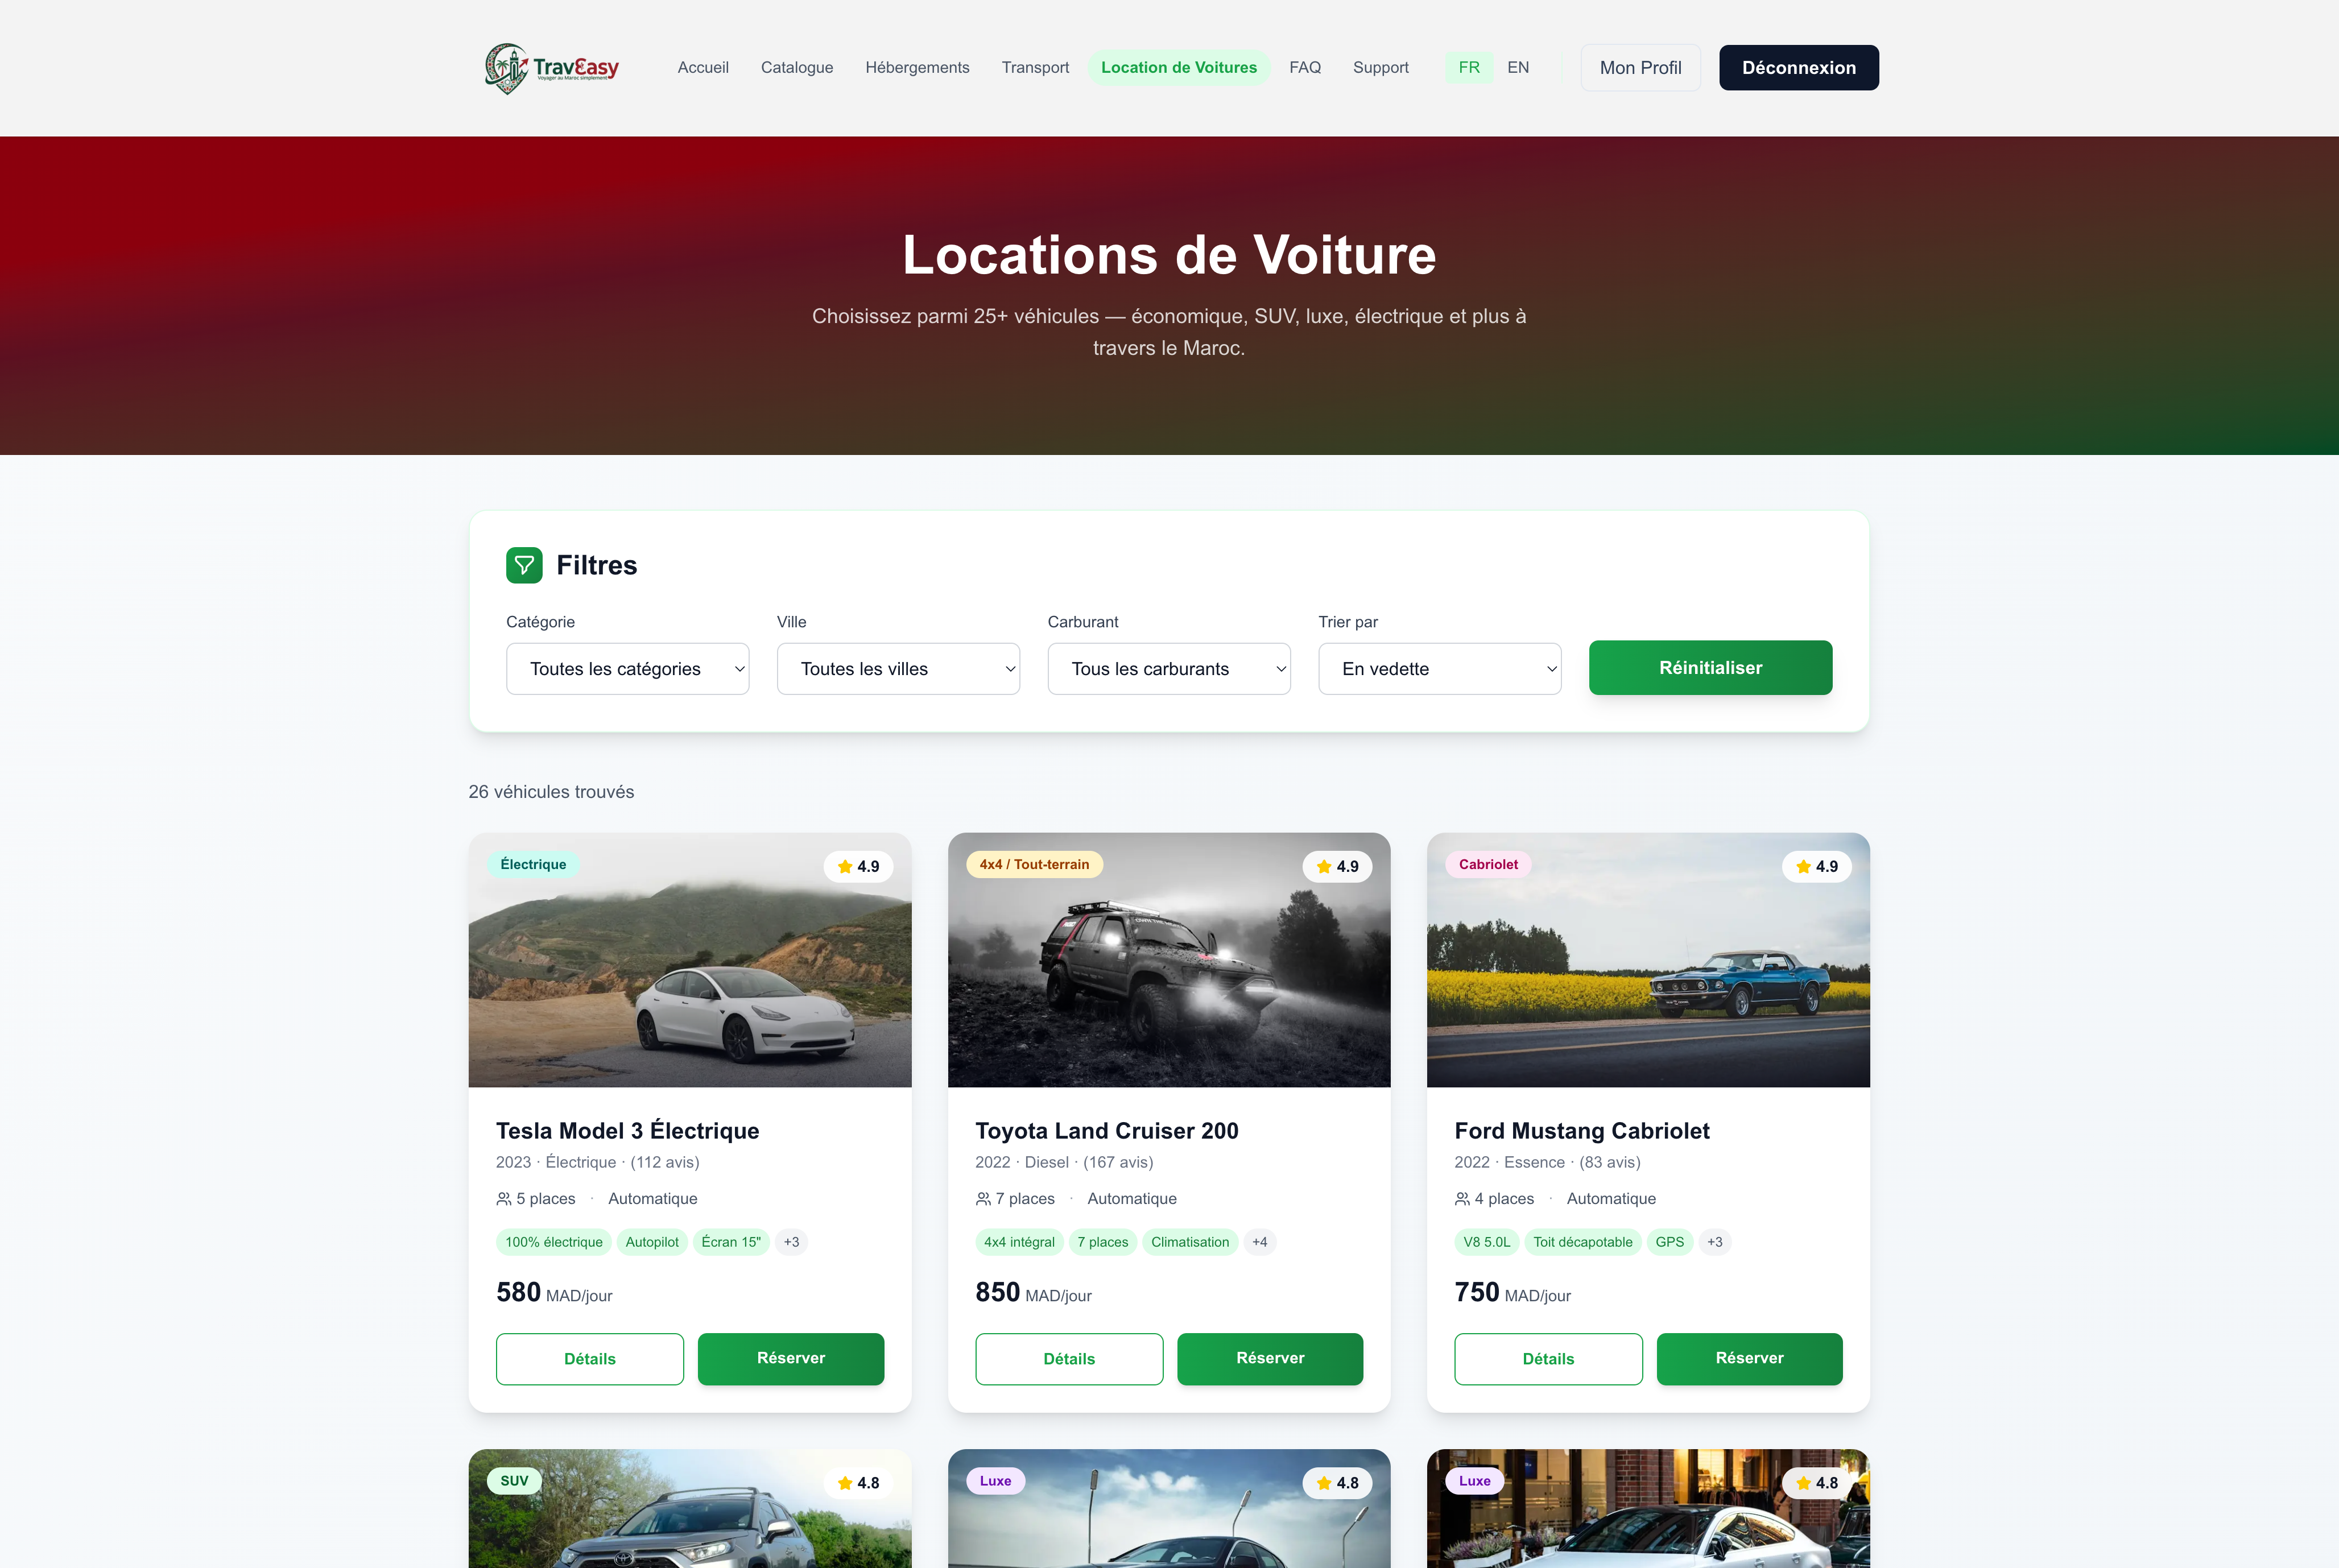
\includegraphics[width=\textwidth]{location.png}
\caption{Page de location de voiture}
\label{fig:Page de location de voiture}
\end{figure}

La page de location de voiture présente les véhicules disponibles sur la plateforme. L'utilisateur peut filtrer les résultats selon le type de véhicule, le prix ou les options, et consulter la disponibilité de chaque véhicule avant d'effectuer une réservation en ligne.

%Affichage des détails du véhicule
\begin{figure}[H]
\centering
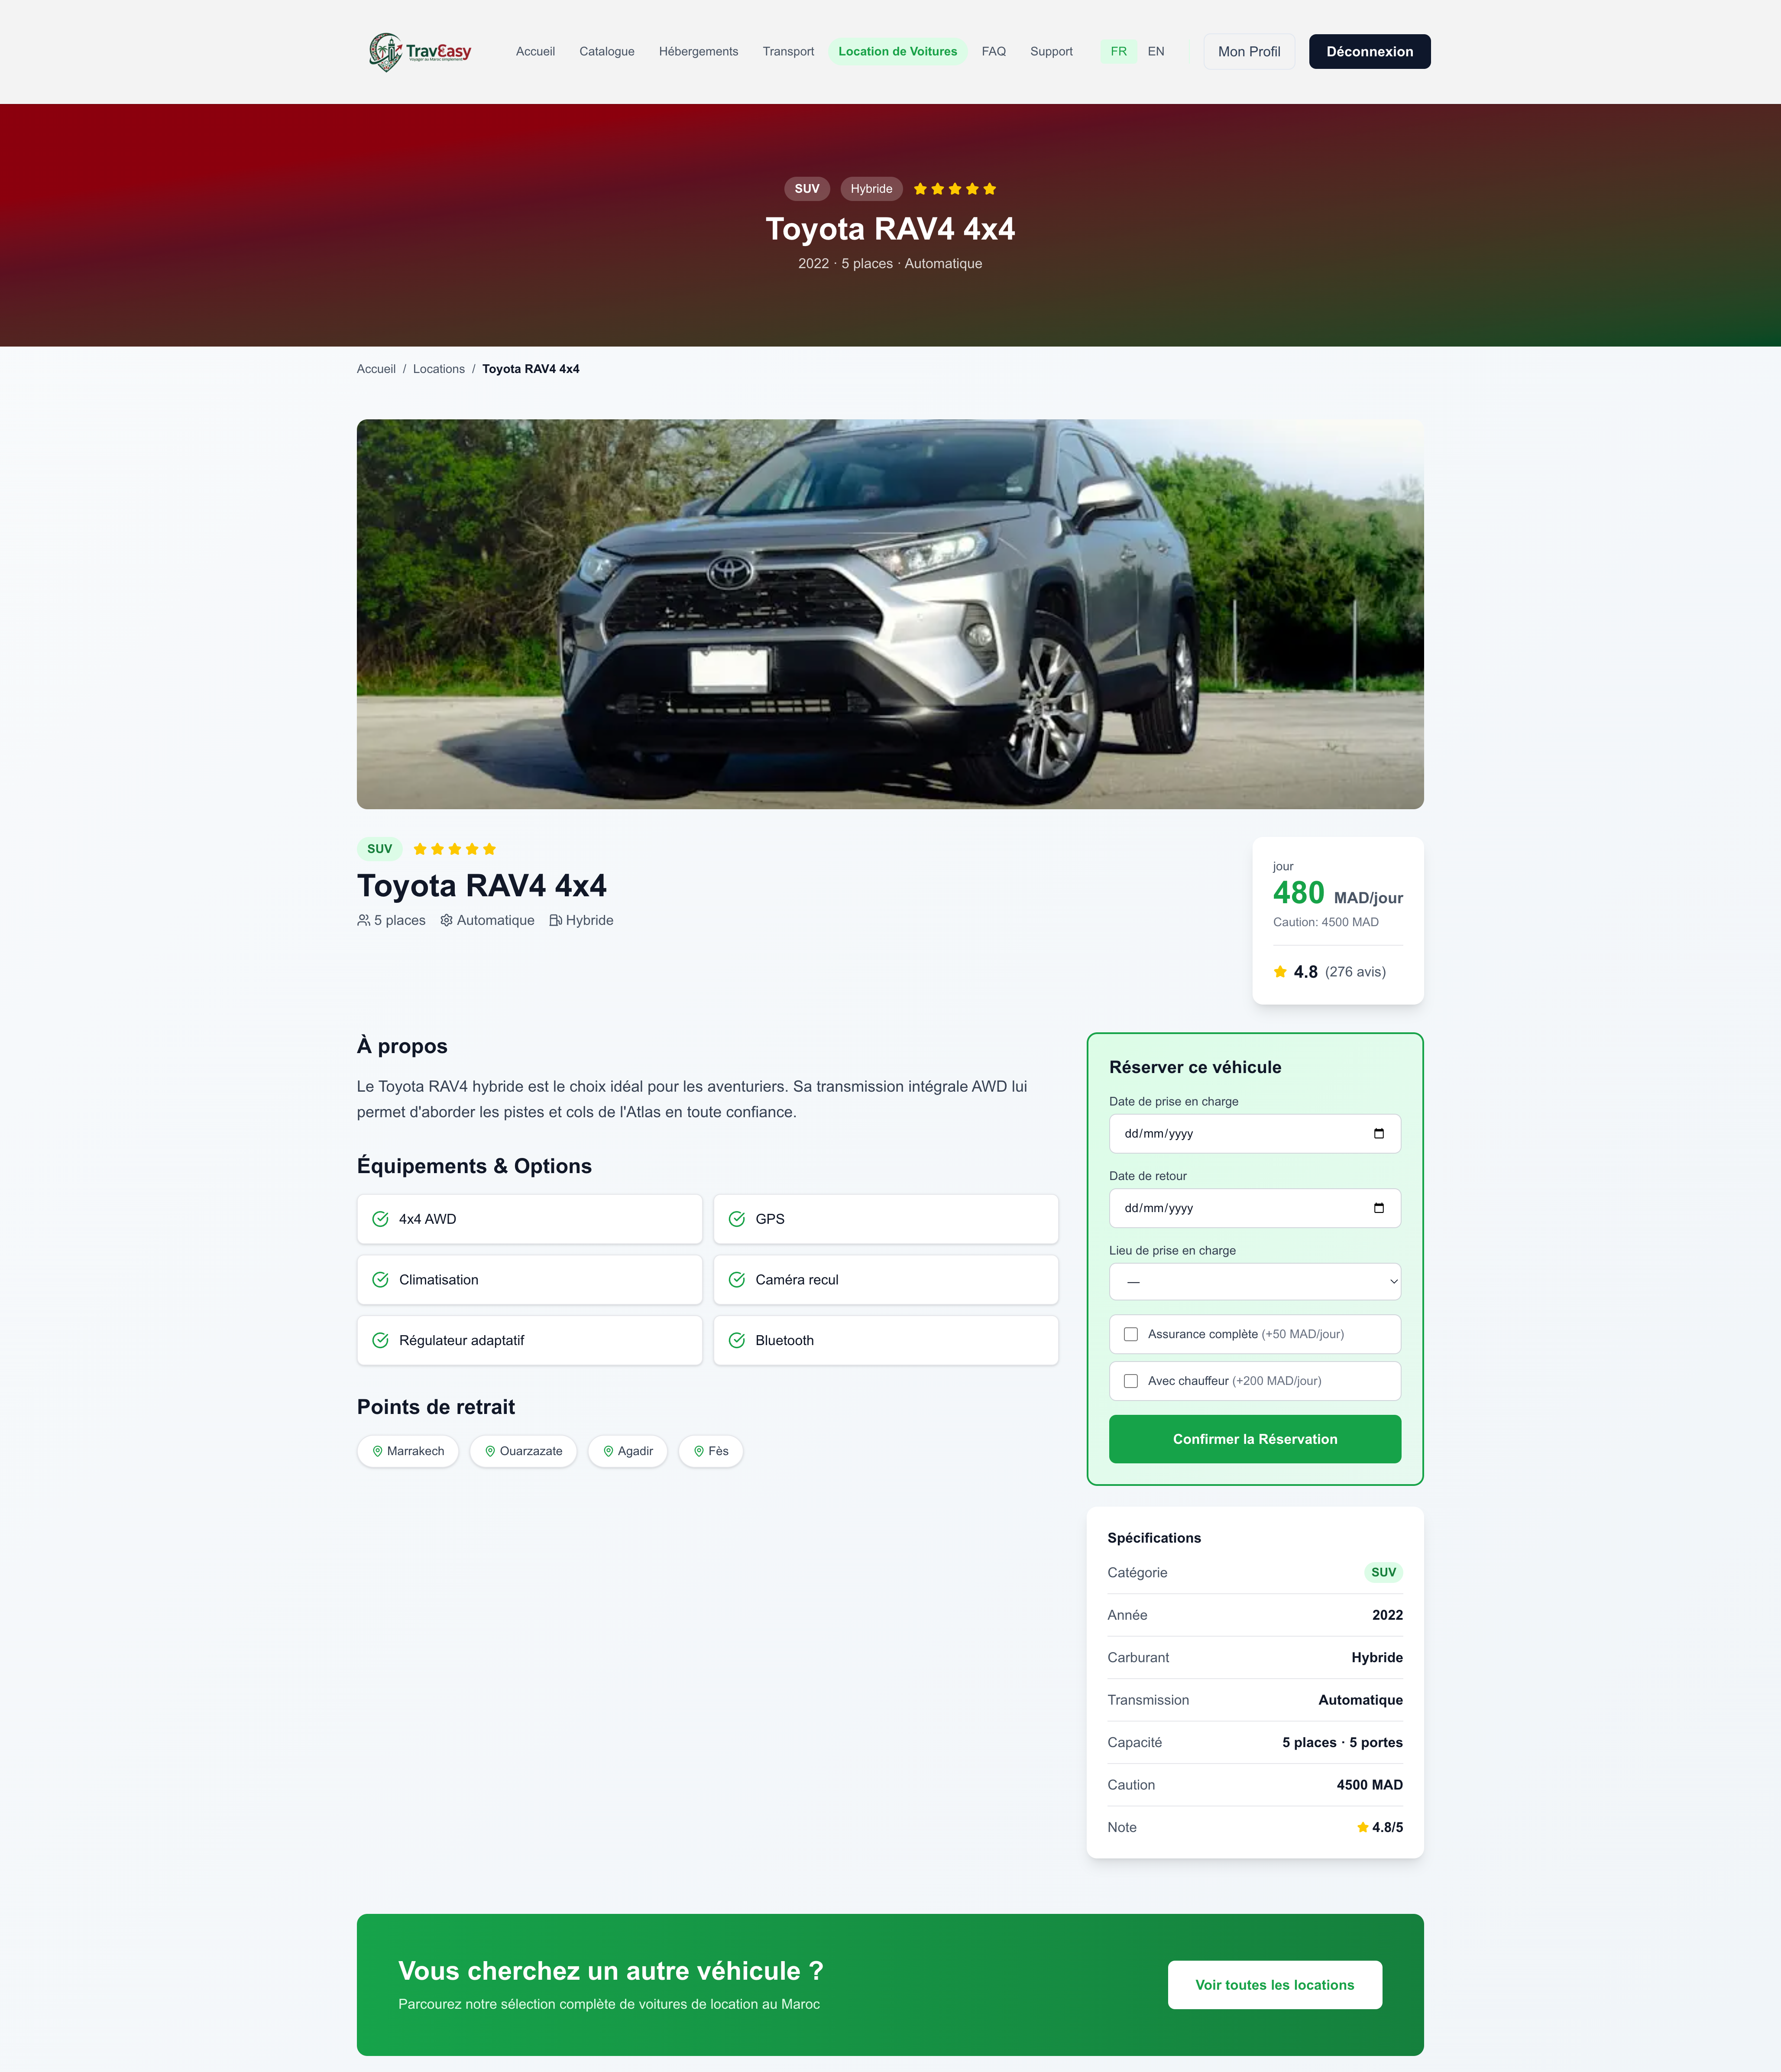
\includegraphics[width=\textwidth]{voit det.png}
\caption{Exemple de détail de véhicule}
\label{fig:Exemple de détail de véhicule}
\end{figure}


Cette figure présente la fiche détaillée d'un véhicule disponible à la location, incluant ses caractéristiques, les options disponibles et le calcul automatique du coût total selon la durée et les options choisies.

\end{spacing}

\subsection{Module de paiement}
\vspace{0.5cm}
\begin{spacing}{1.5}
\justifying
Le module de paiement a été développé afin de permettre aux utilisateurs d’effectuer leurs transactions en ligne de manière simple et sécurisée. Il intègre des mécanismes de \textbf{paiement sécurisé} reposant sur l’utilisation de passerelles de paiement fiables telles que Stripe ou PayPal, garantissant la protection des données financières des utilisateurs. Une fois le paiement effectué, le système procède à la \textbf{validation de la transaction} afin de vérifier son succès avant de confirmer définitivement la réservation concernée. Le module assure également la \textbf{génération automatique d’une facture au format PDF}, permettant à l’utilisateur de conserver une preuve de paiement et de consulter les détails de sa transaction à tout moment. Cette fonctionnalité contribue à renforcer la transparence, la fiabilité et la traçabilité des opérations financières réalisées sur la plateforme.
%Page paiement
\begin{figure}[H]
\centering
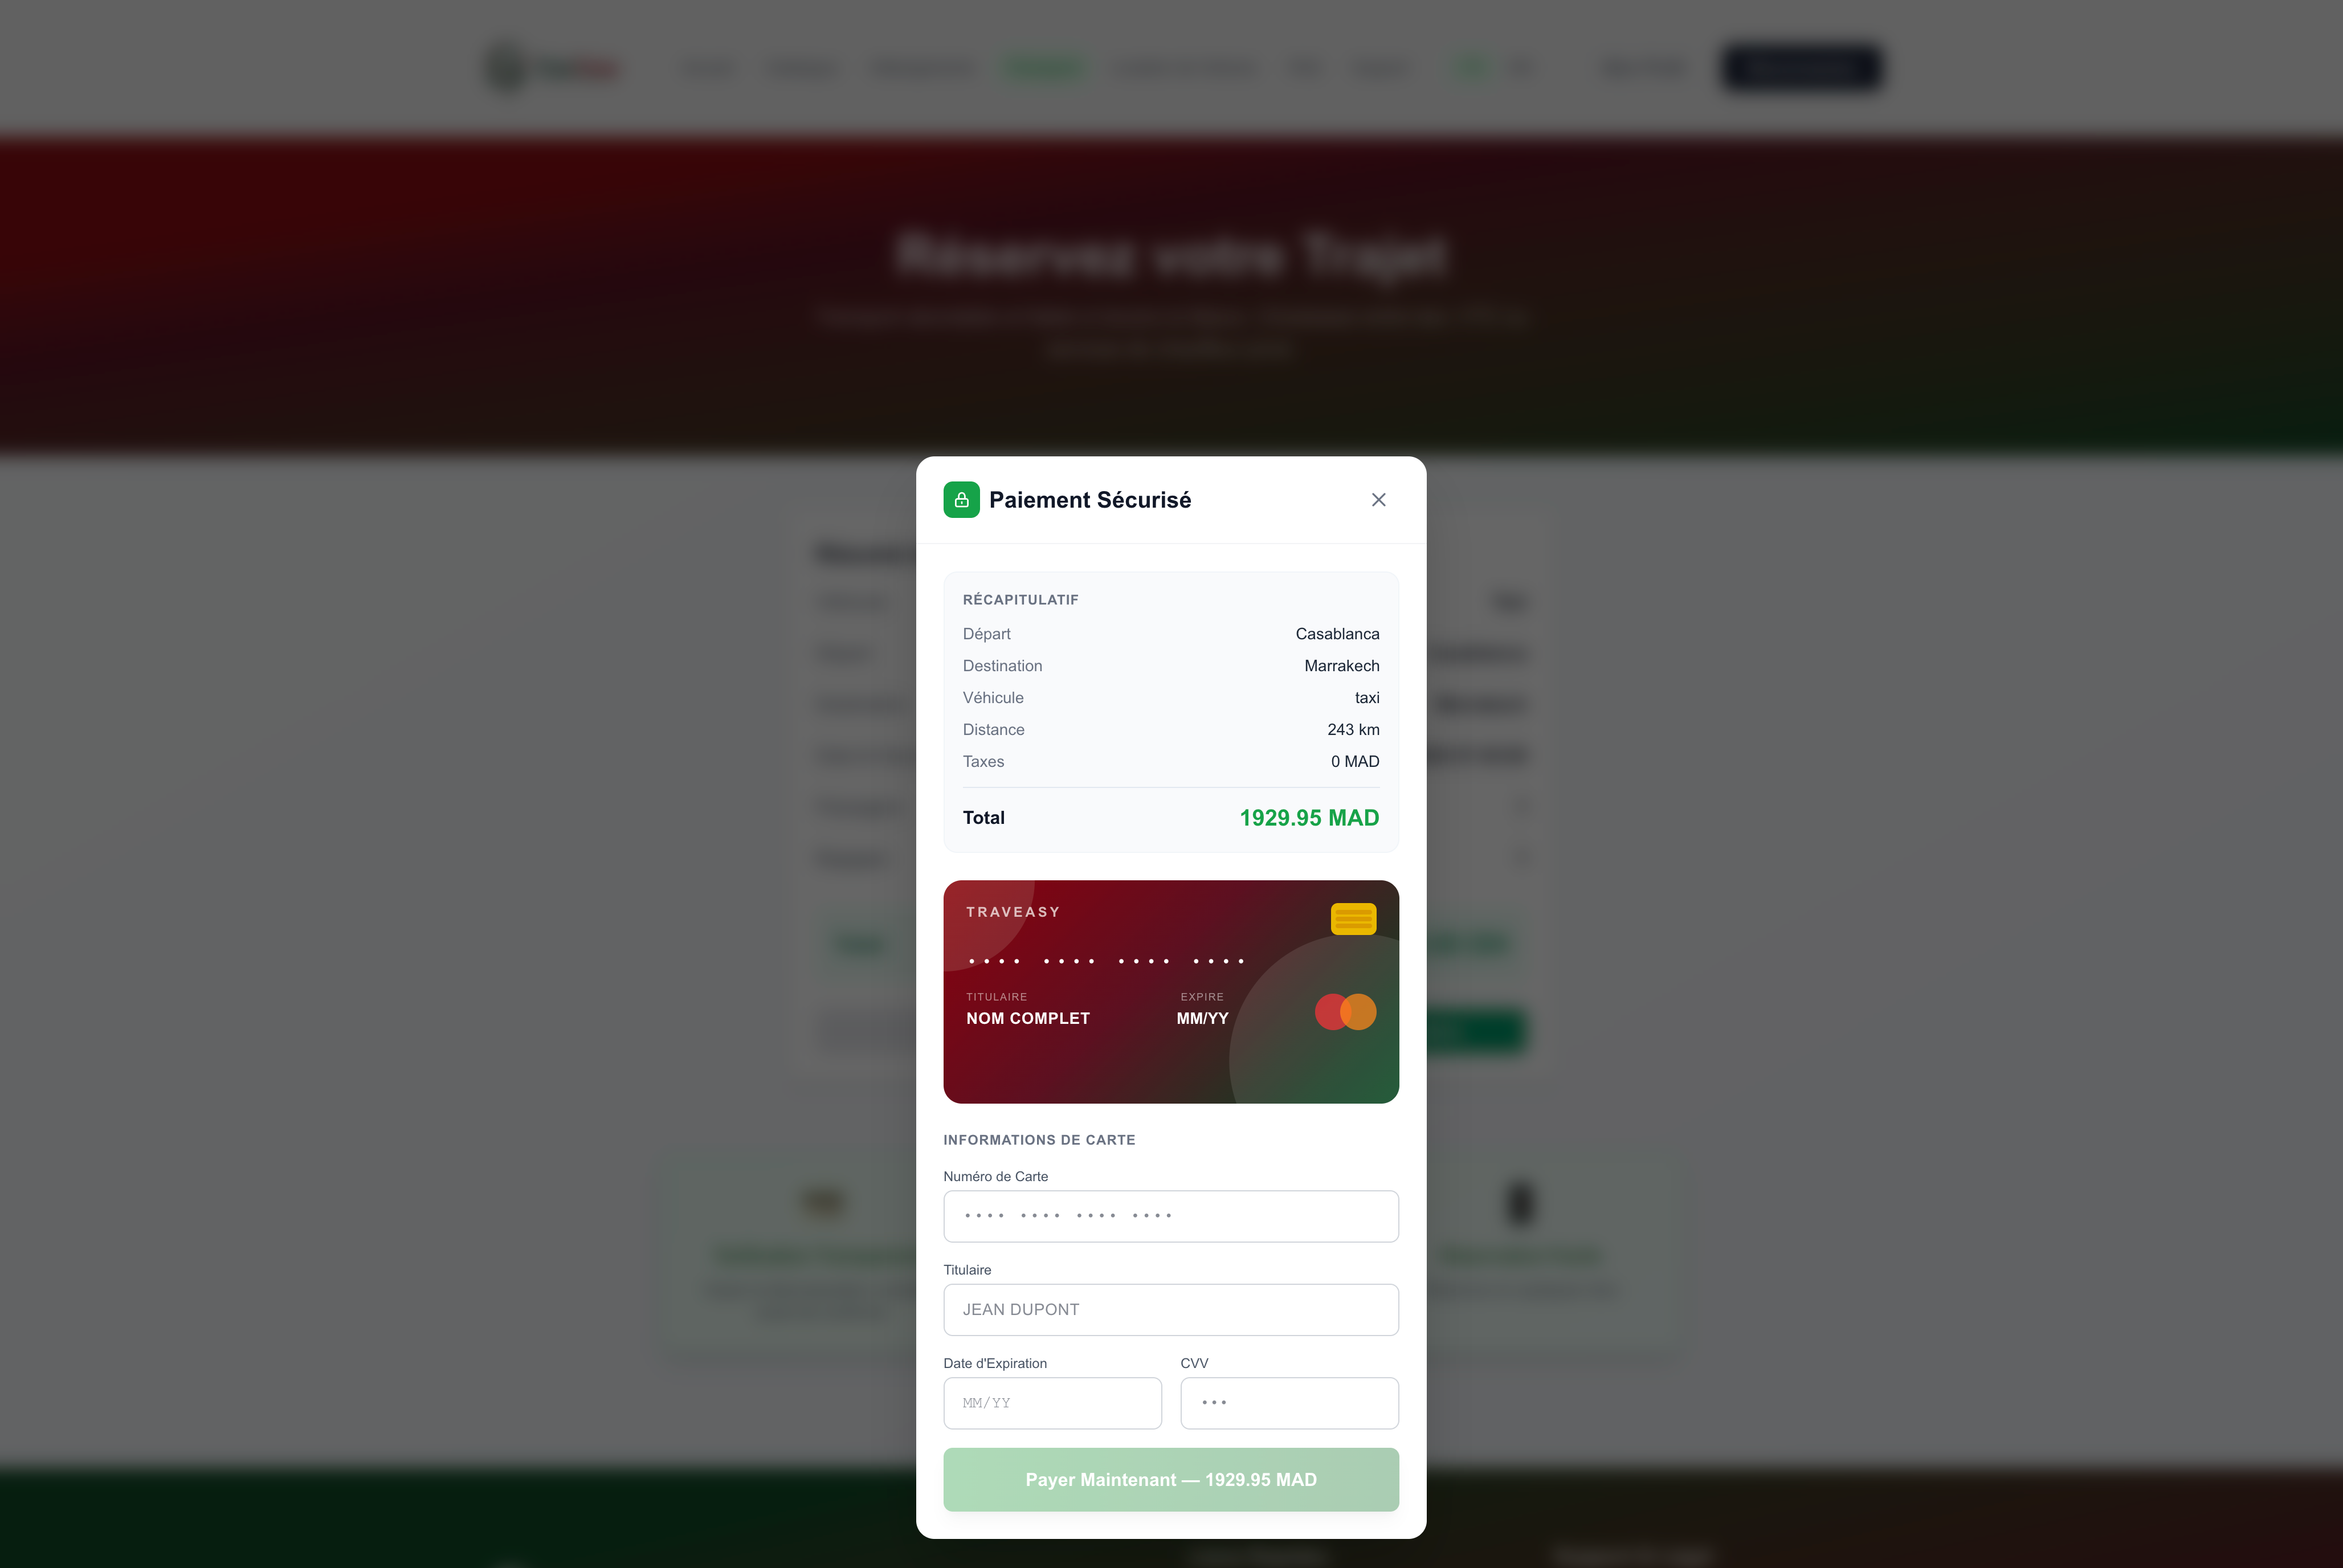
\includegraphics[width=\textwidth]{payment.png}
\caption{Page de paiement}
\label{fig:Page de paiement}
\end{figure}

La page de paiement permet aux utilisateurs de finaliser leurs transactions en ligne de manière sécurisée, via des passerelles de paiement fiables telles que Stripe ou PayPal. Le montant et les détails de la réservation sont affichés clairement avant confirmation.

%Exemple de facture générée
\begin{figure}[H]
\centering
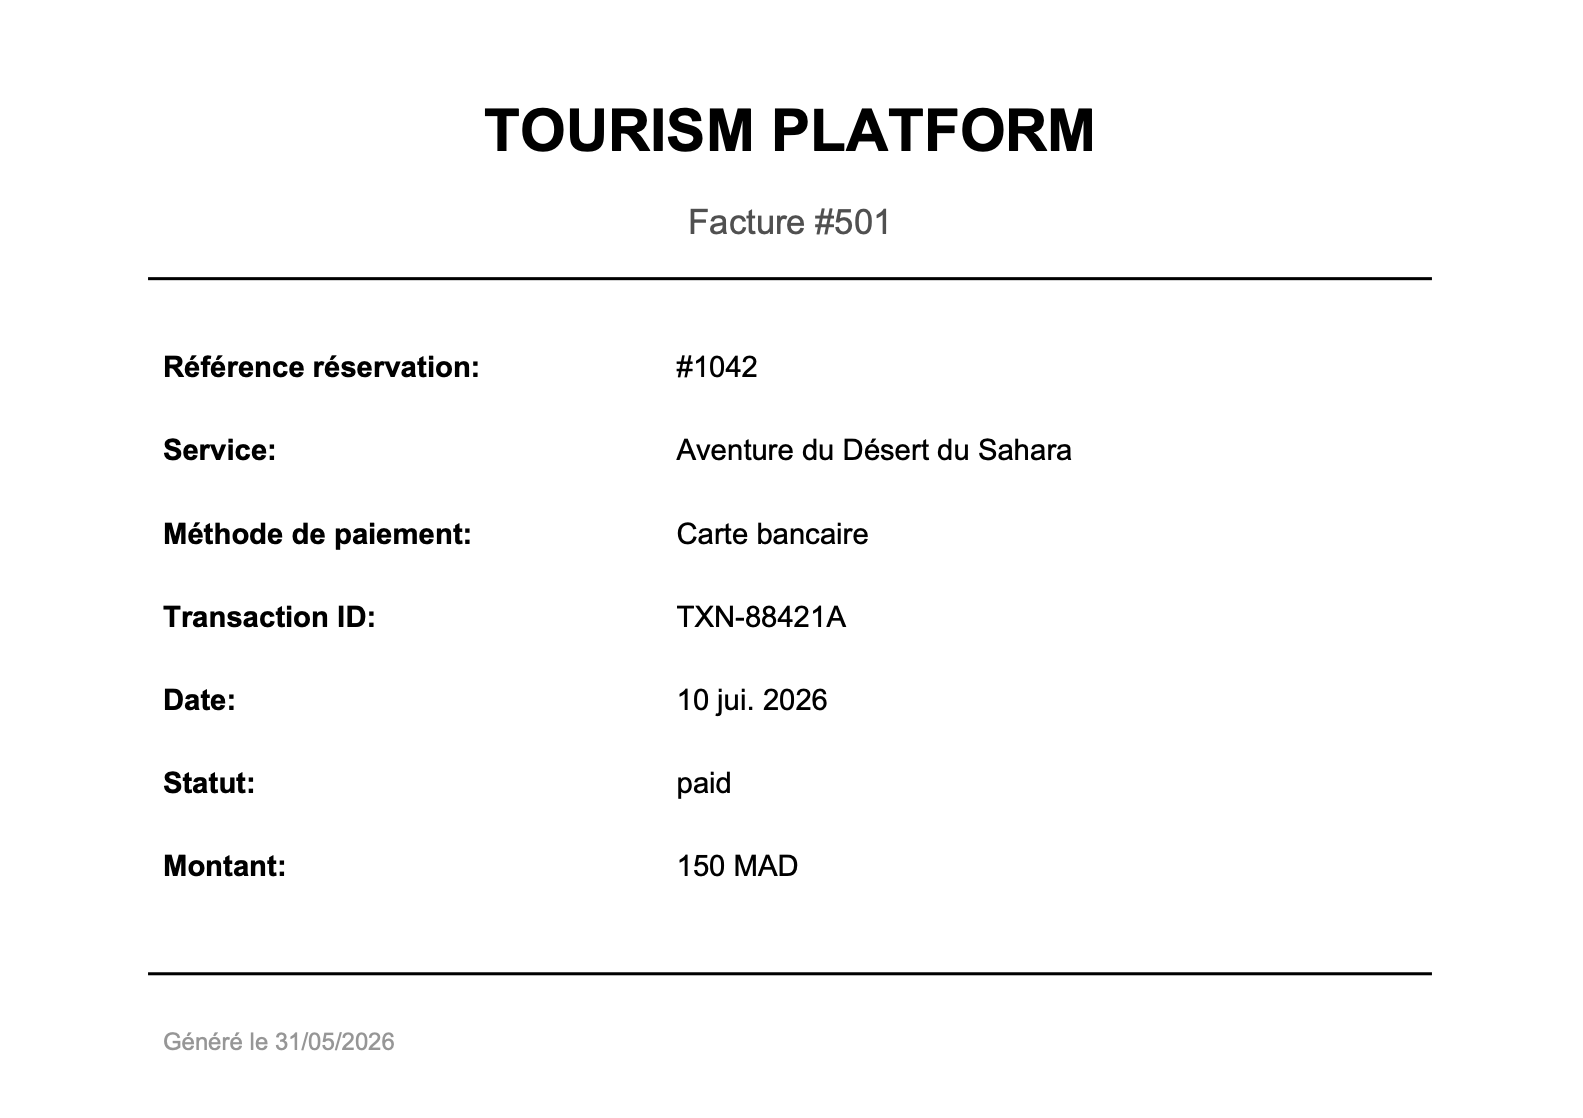
\includegraphics[width=\textwidth]{facture.png}
\caption{Exemple de facture générée}
\label{fig:Exemple de facture générée}
\end{figure}

À la suite d'un paiement validé, le système génère automatiquement une facture au format PDF. Cette figure illustre un exemple de facture produite, permettant à l'utilisateur de conserver une preuve de paiement et de consulter les détails de sa transaction.

\end{spacing}

\subsection{Module d’avis et de notation}
\vspace{0.5cm}
\begin{spacing}{1.5}
\justifying
Le module d’avis et de notation permet aux utilisateurs de partager leurs expériences et d’évaluer les différents services proposés sur la plateforme. Après avoir utilisé un service ou effectué une réservation, l’utilisateur peut \textbf{ajouter} un avis afin d’exprimer son niveau de satisfaction et fournir des retours utiles aux autres utilisateurs. Le système offre également la possibilité d’\textbf{attribuer une note} à chaque service, permettant ainsi d’évaluer sa qualité de manière quantitative. Afin de fournir une appréciation globale et objective, la plateforme effectue automatiquement le \textbf{calcul de la note moyenne} à partir de l’ensemble des évaluations reçues. Ce module favorise la transparence, renforce la confiance des utilisateurs et contribue à améliorer la qualité des services proposés.

%Affichage des évaluations
\begin{figure}[H]
\centering
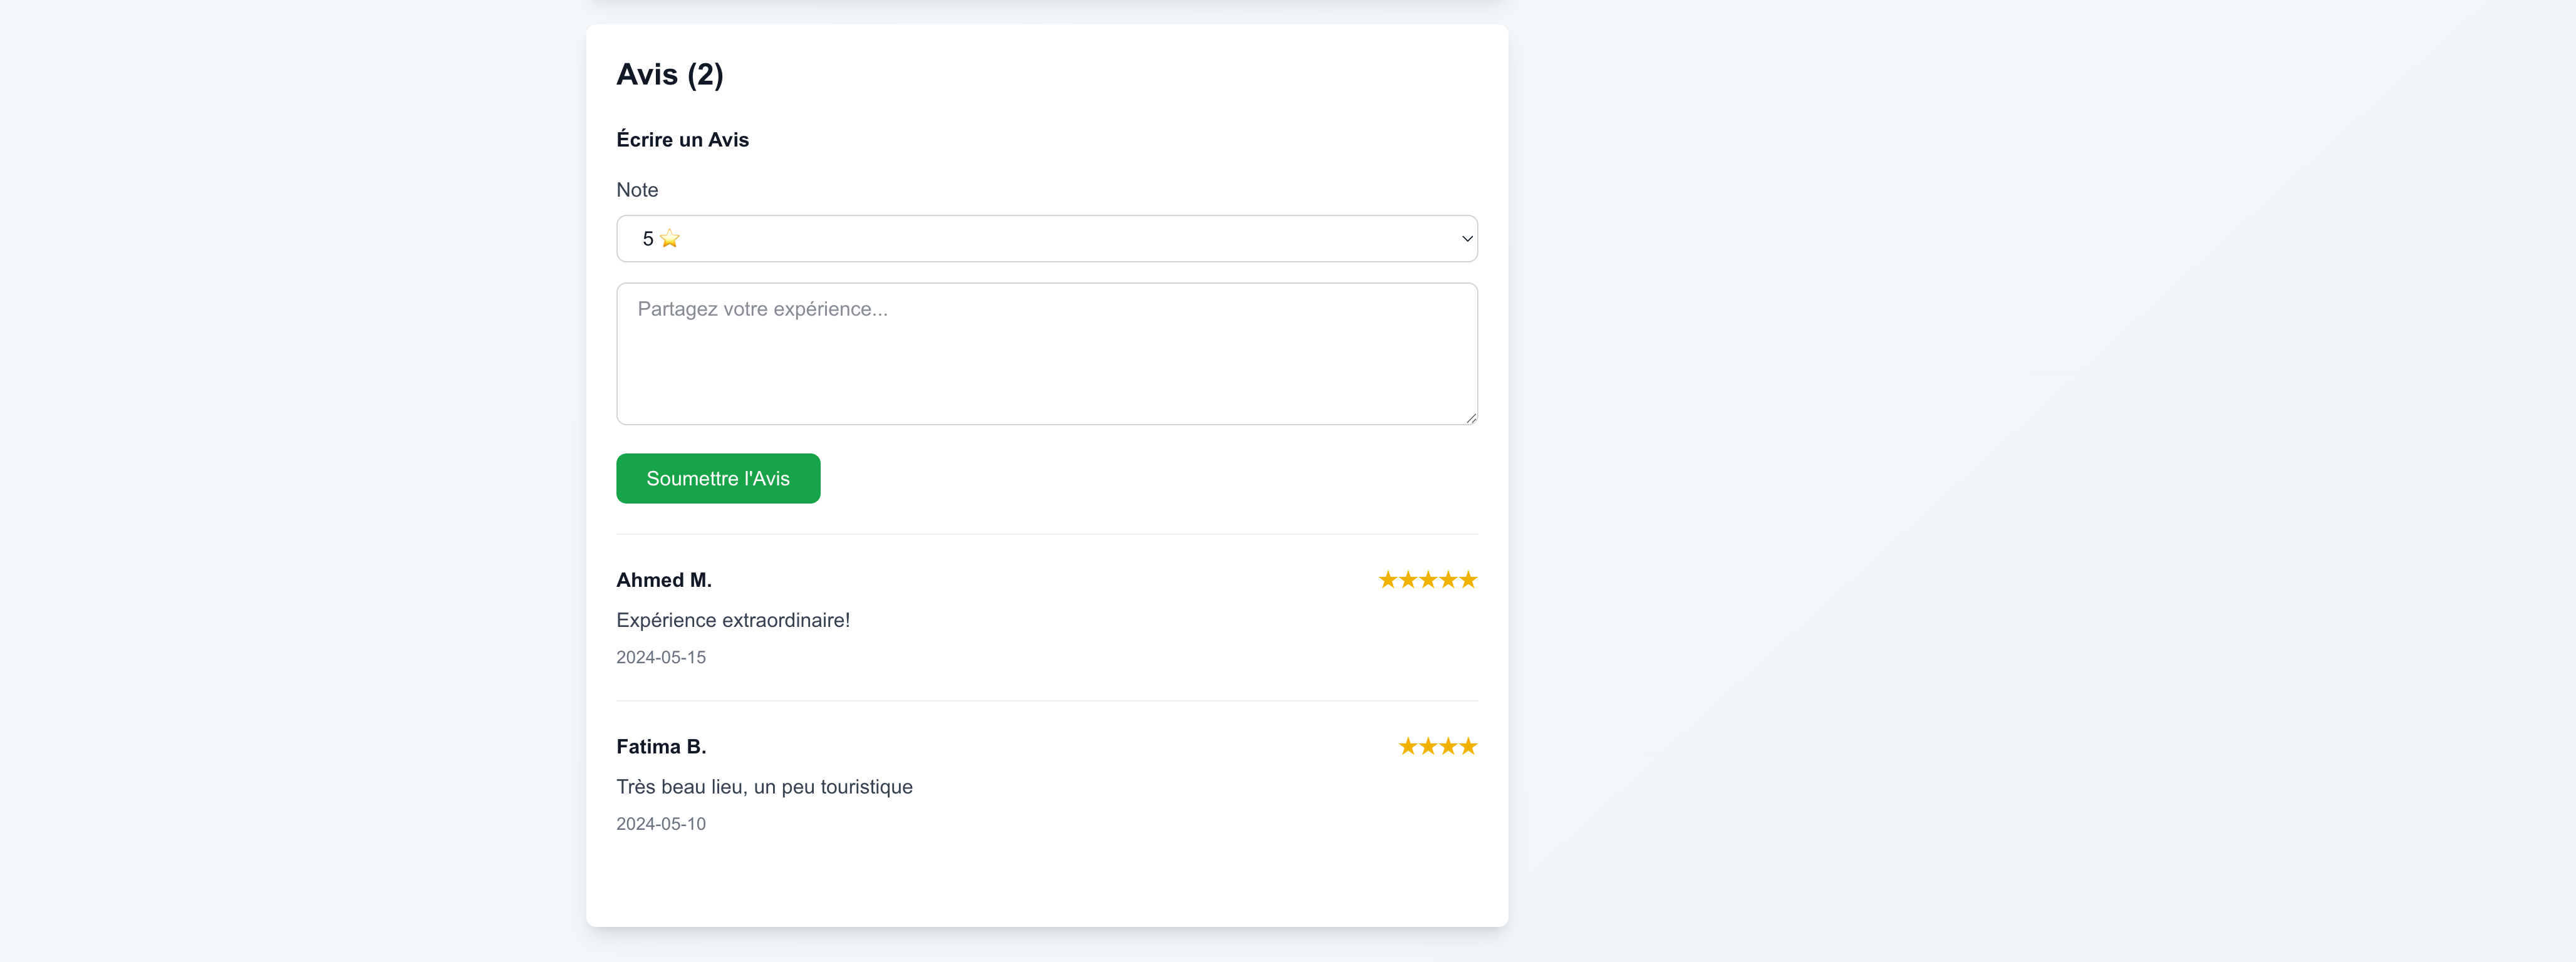
\includegraphics[width=\textwidth]{avis.png}
\caption{Exemple d'avis et de notation}
\label{fig:Exemple d'avis et de notation}
\end{figure}


Cette figure illustre le module d'avis et de notation, permettant aux utilisateurs d'évaluer les services utilisés et de laisser des commentaires. La plateforme calcule automatiquement la note moyenne afin de fournir une appréciation globale et objective de chaque service.

\end{spacing}

\subsection{Espace profil utilisateur}
\vspace{0.5cm}
\begin{spacing}{1.5}
\justifying
L’espace profil regroupe dans une interface unique les informations personnelles et les principales données liées au compte utilisateur. Ce module a été conçu pour offrir une gestion centralisée, simple et claire des éléments essentiels du parcours utilisateur.

Depuis cette section, l’utilisateur peut consulter et modifier ses informations de profil (nom, prénom, langue), accéder à l’historique de ses \textbf{réservations}, visualiser ses \textbf{paiements} ainsi que gérer ses \textbf{préférences}. Cette organisation améliore l’expérience utilisateur en facilitant l’accès rapide aux informations importantes sans naviguer entre plusieurs pages.

\begin{figure}[H]
\centering
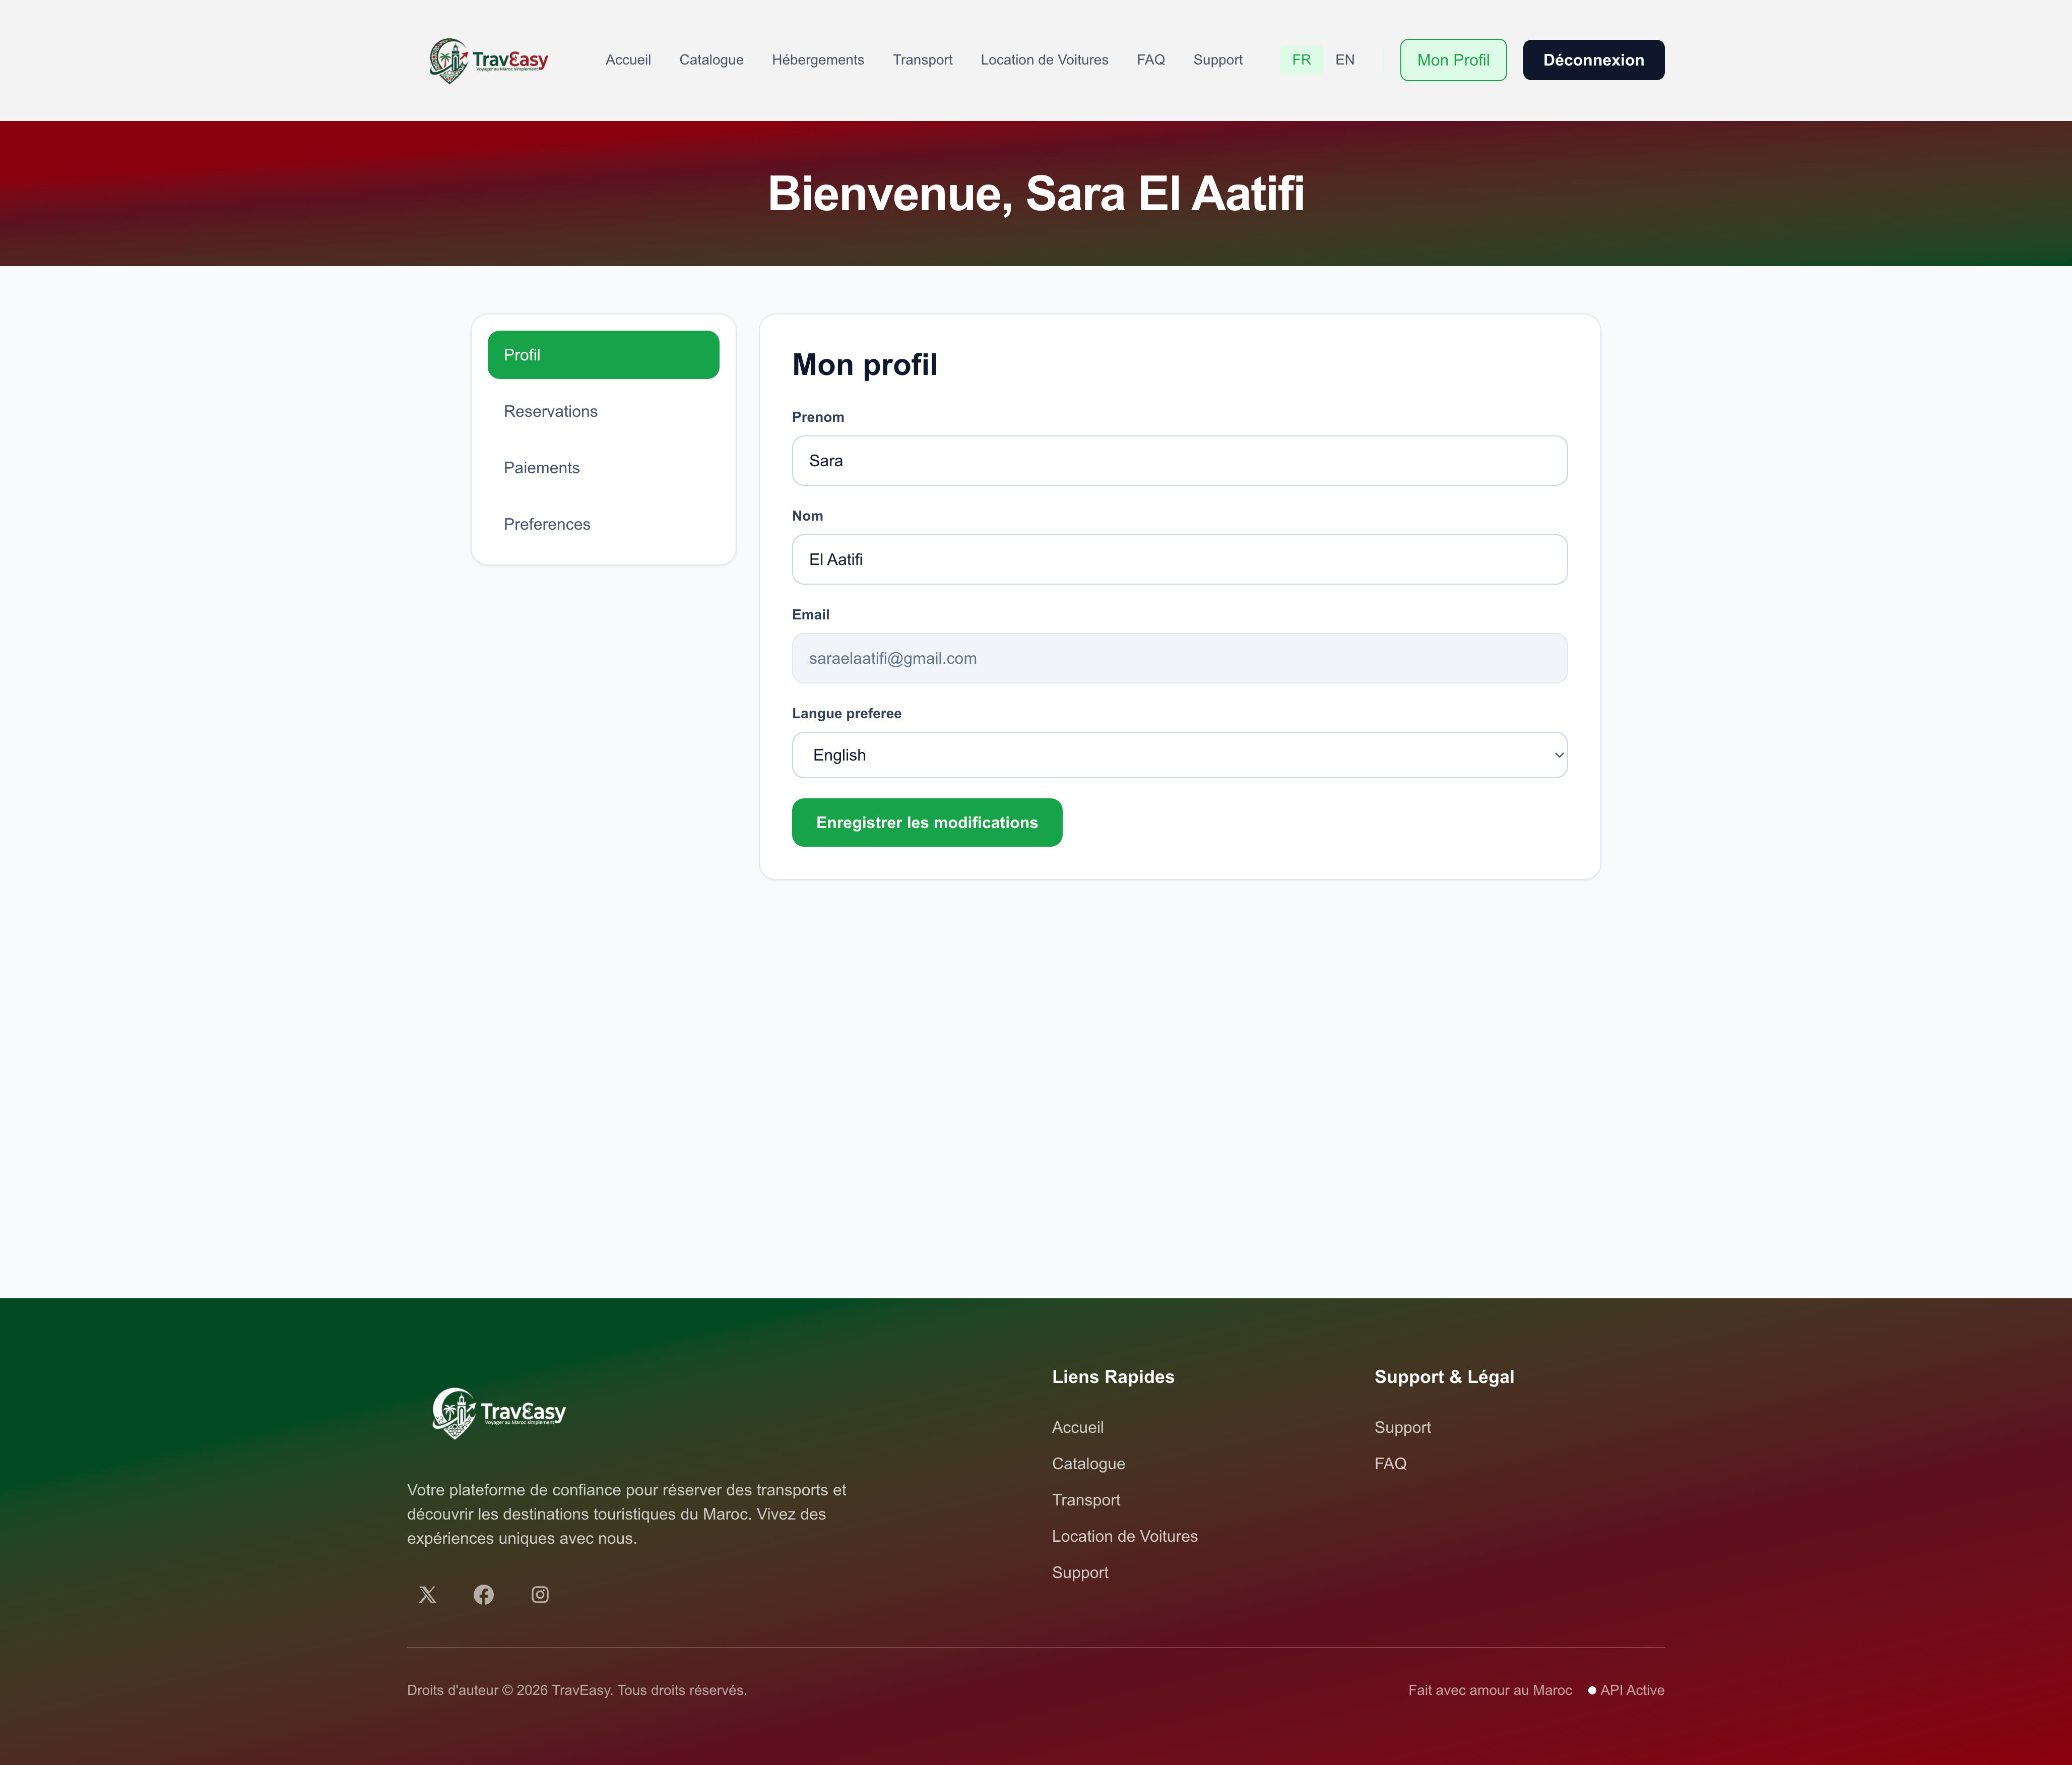
\includegraphics[width=\textwidth]{profile.png}
\caption{Espace profil utilisateur}
\label{fig:Espace profil utilisateur}
\end{figure}

L'espace profil regroupe dans une interface unique les informations personnelles de l'utilisateur (nom, prénom, langue) ainsi que l'accès à ses réservations, paiements et préférences, offrant une gestion centralisée et simplifiée du compte.

\begin{figure}[H]
\centering
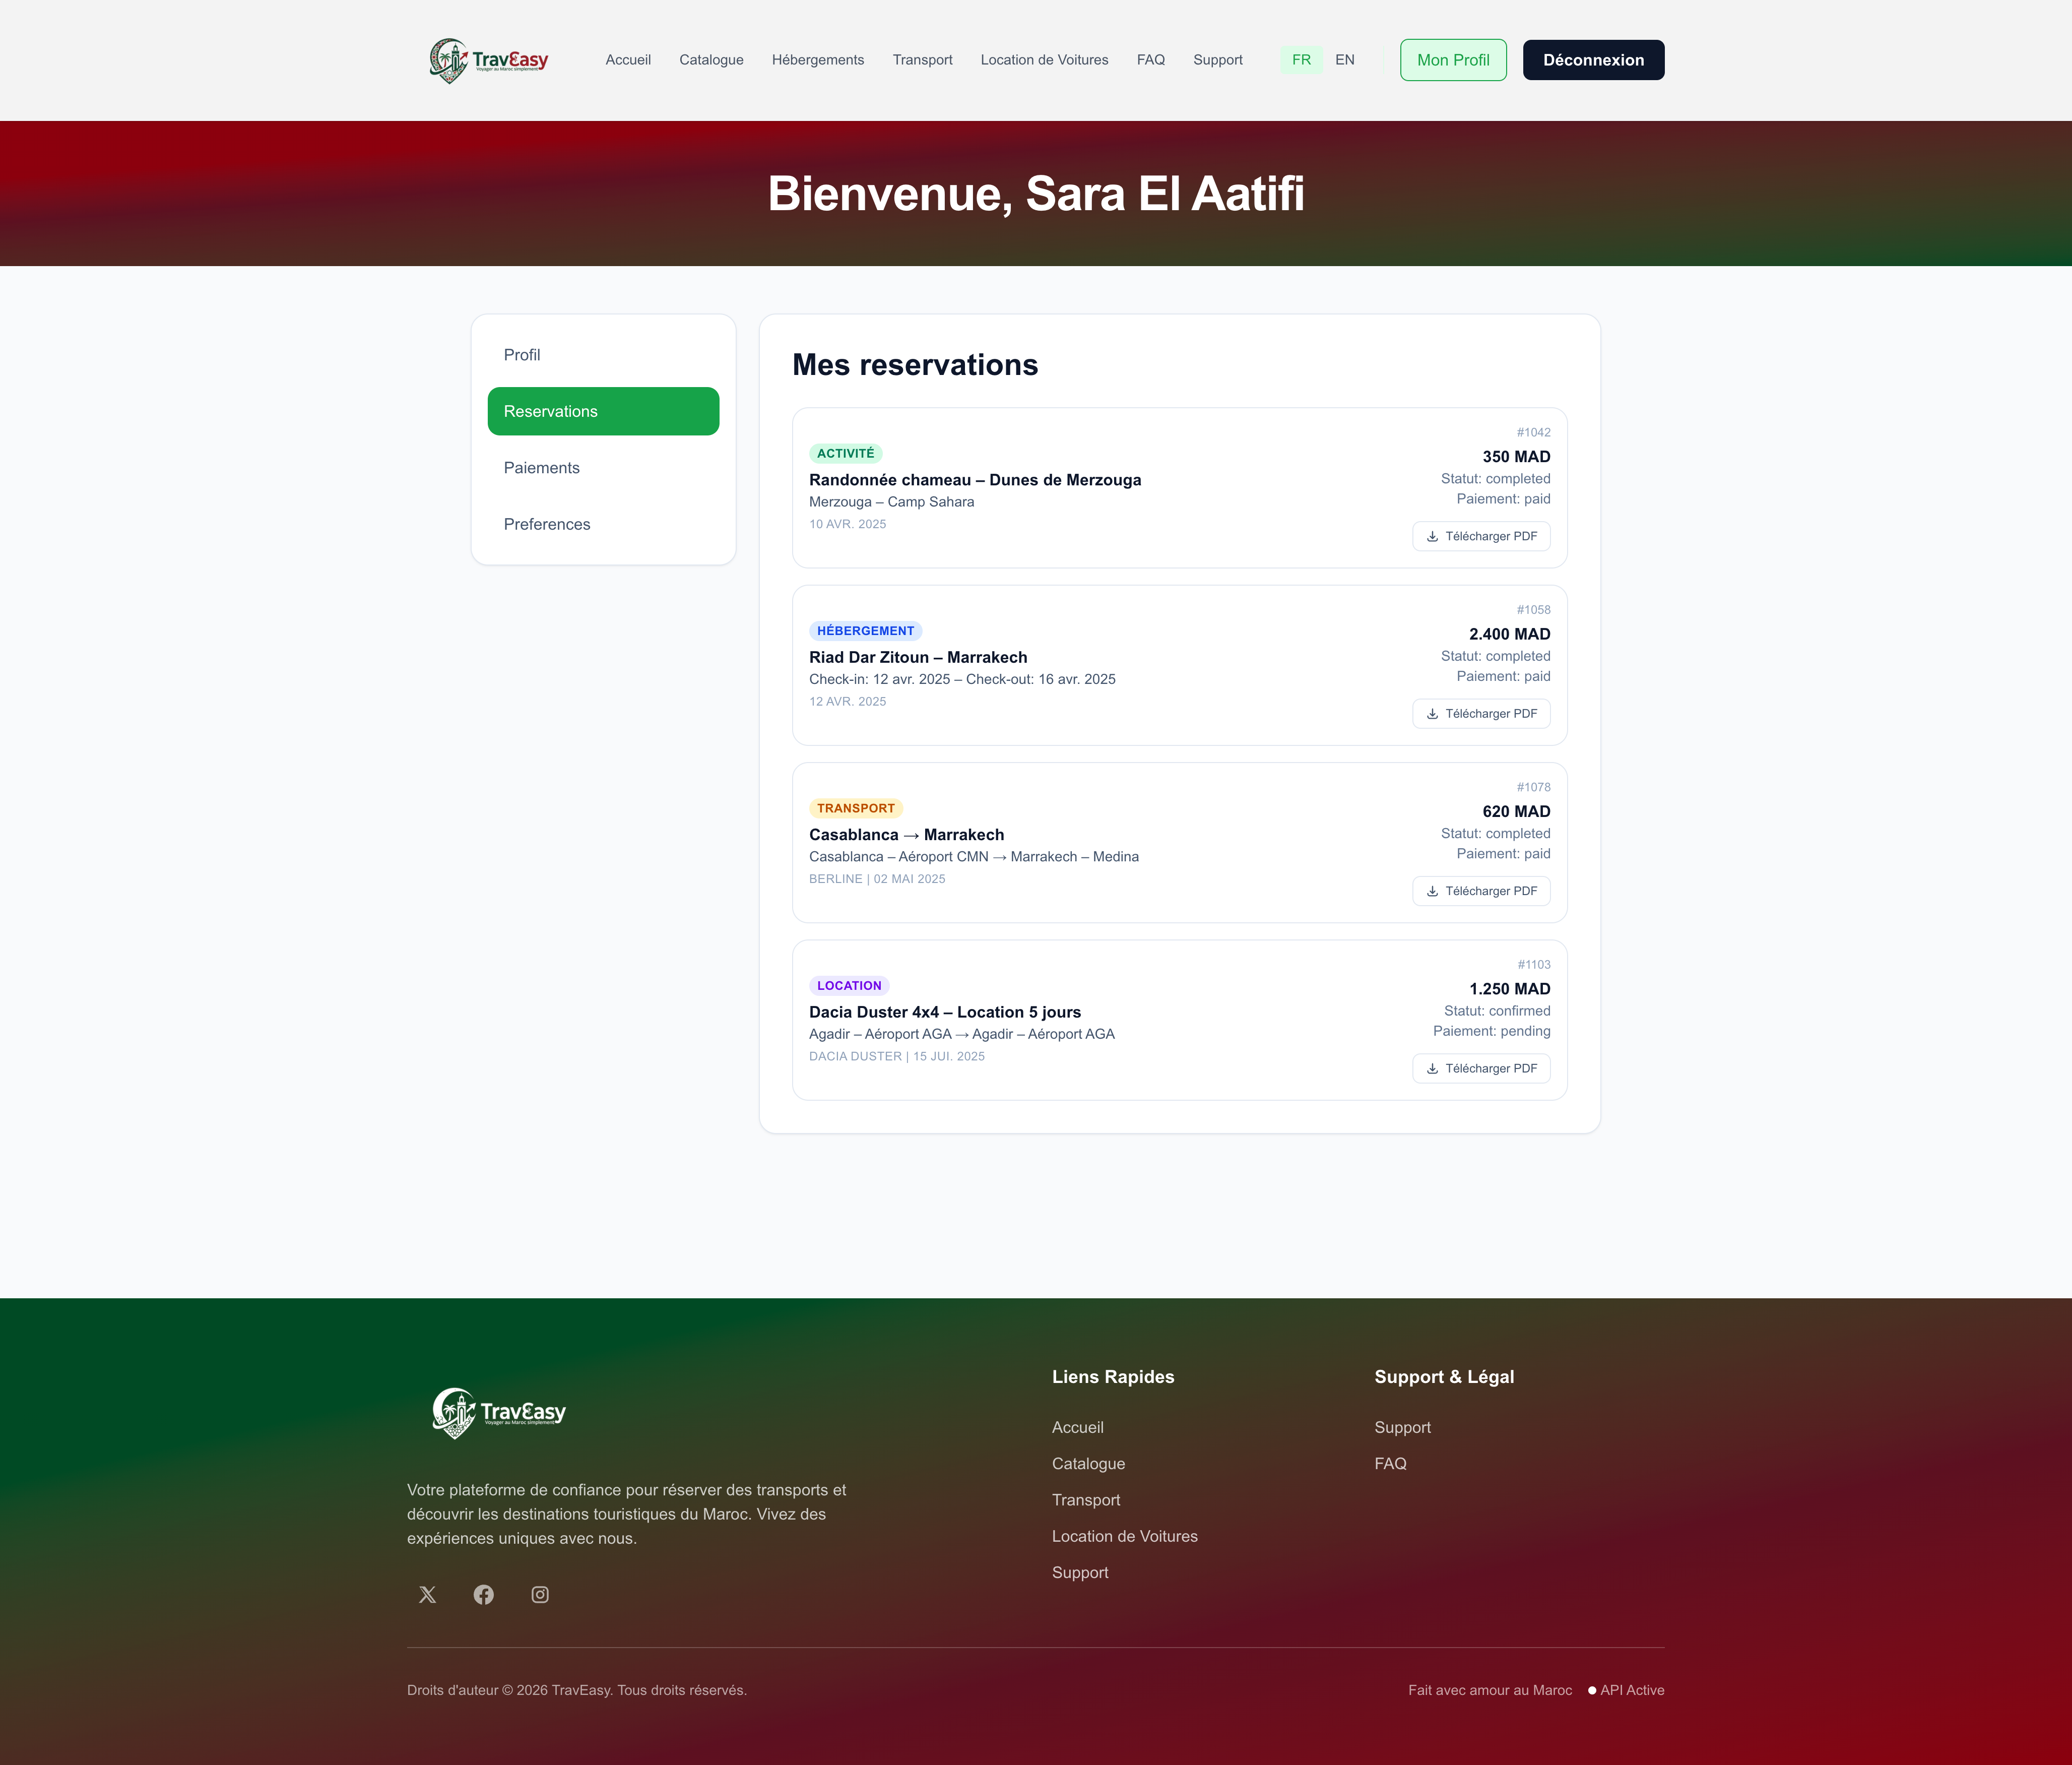
\includegraphics[width=\textwidth]{resa.png}
\caption{Onglet des réservations dans l’espace profil}
\label{fig:Onglet reservations profil}
\end{figure}

Cet onglet permet à l'utilisateur de consulter l'historique complet de ses réservations effectuées sur la plateforme, facilitant le suivi et la gestion de ses activités passées et à venir.

\begin{figure}[H]
\centering
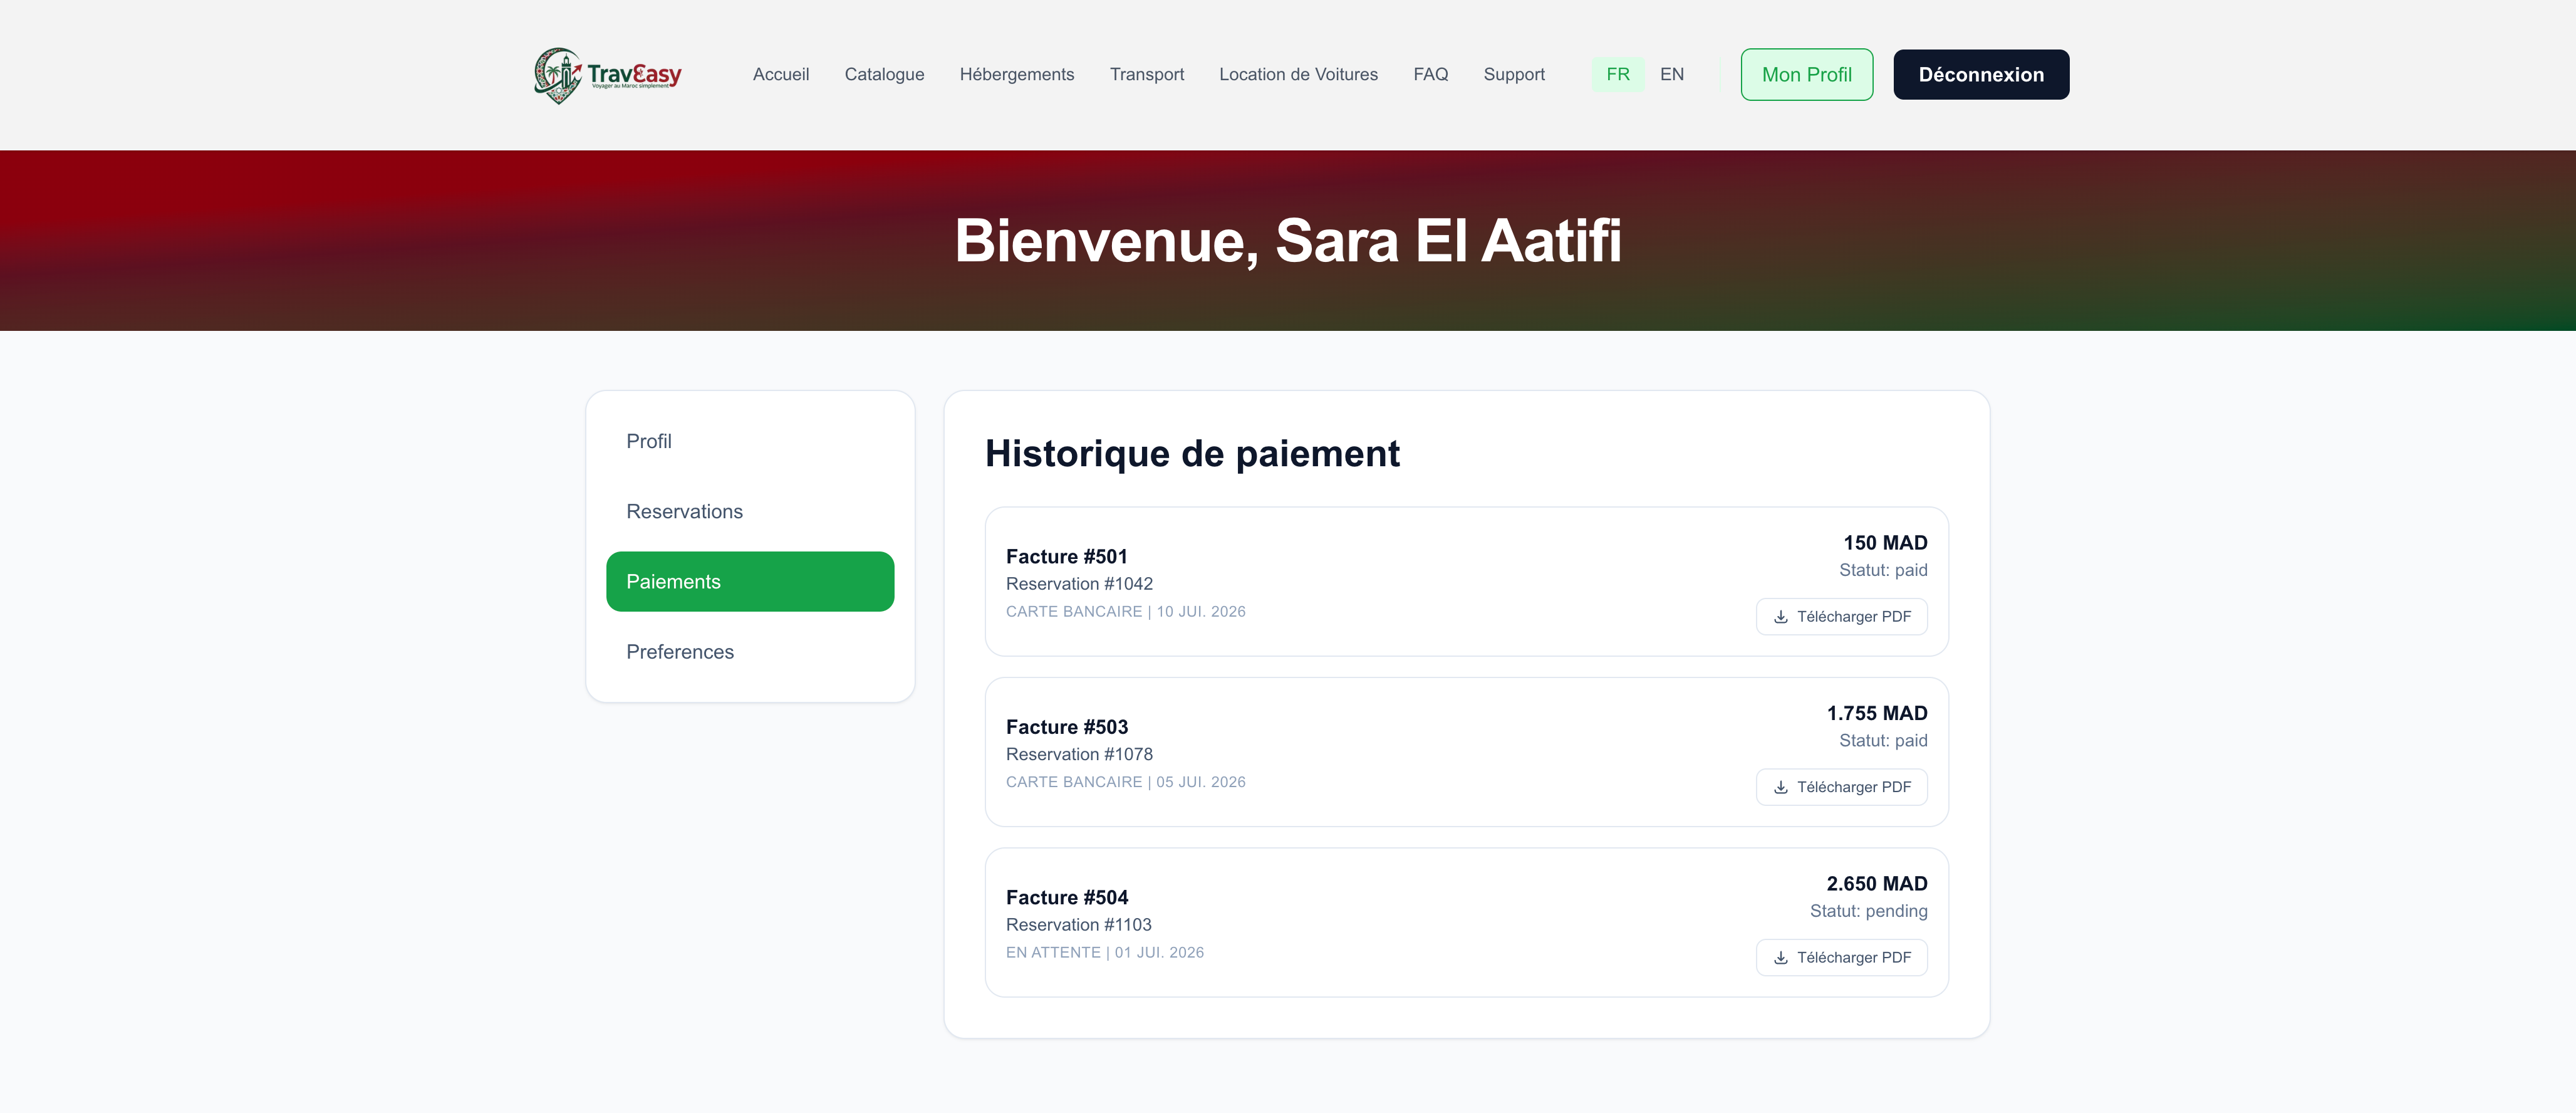
\includegraphics[width=\textwidth]{paie.png}
\caption{Onglet des paiements dans l’espace profil}
\label{fig:Onglet paiements profil}
\end{figure}


Cet onglet donne accès à l'historique des transactions financières de l'utilisateur, lui permettant de visualiser et de suivre l'ensemble de ses paiements réalisés sur la plateforme.

\begin{figure}[H]
\centering
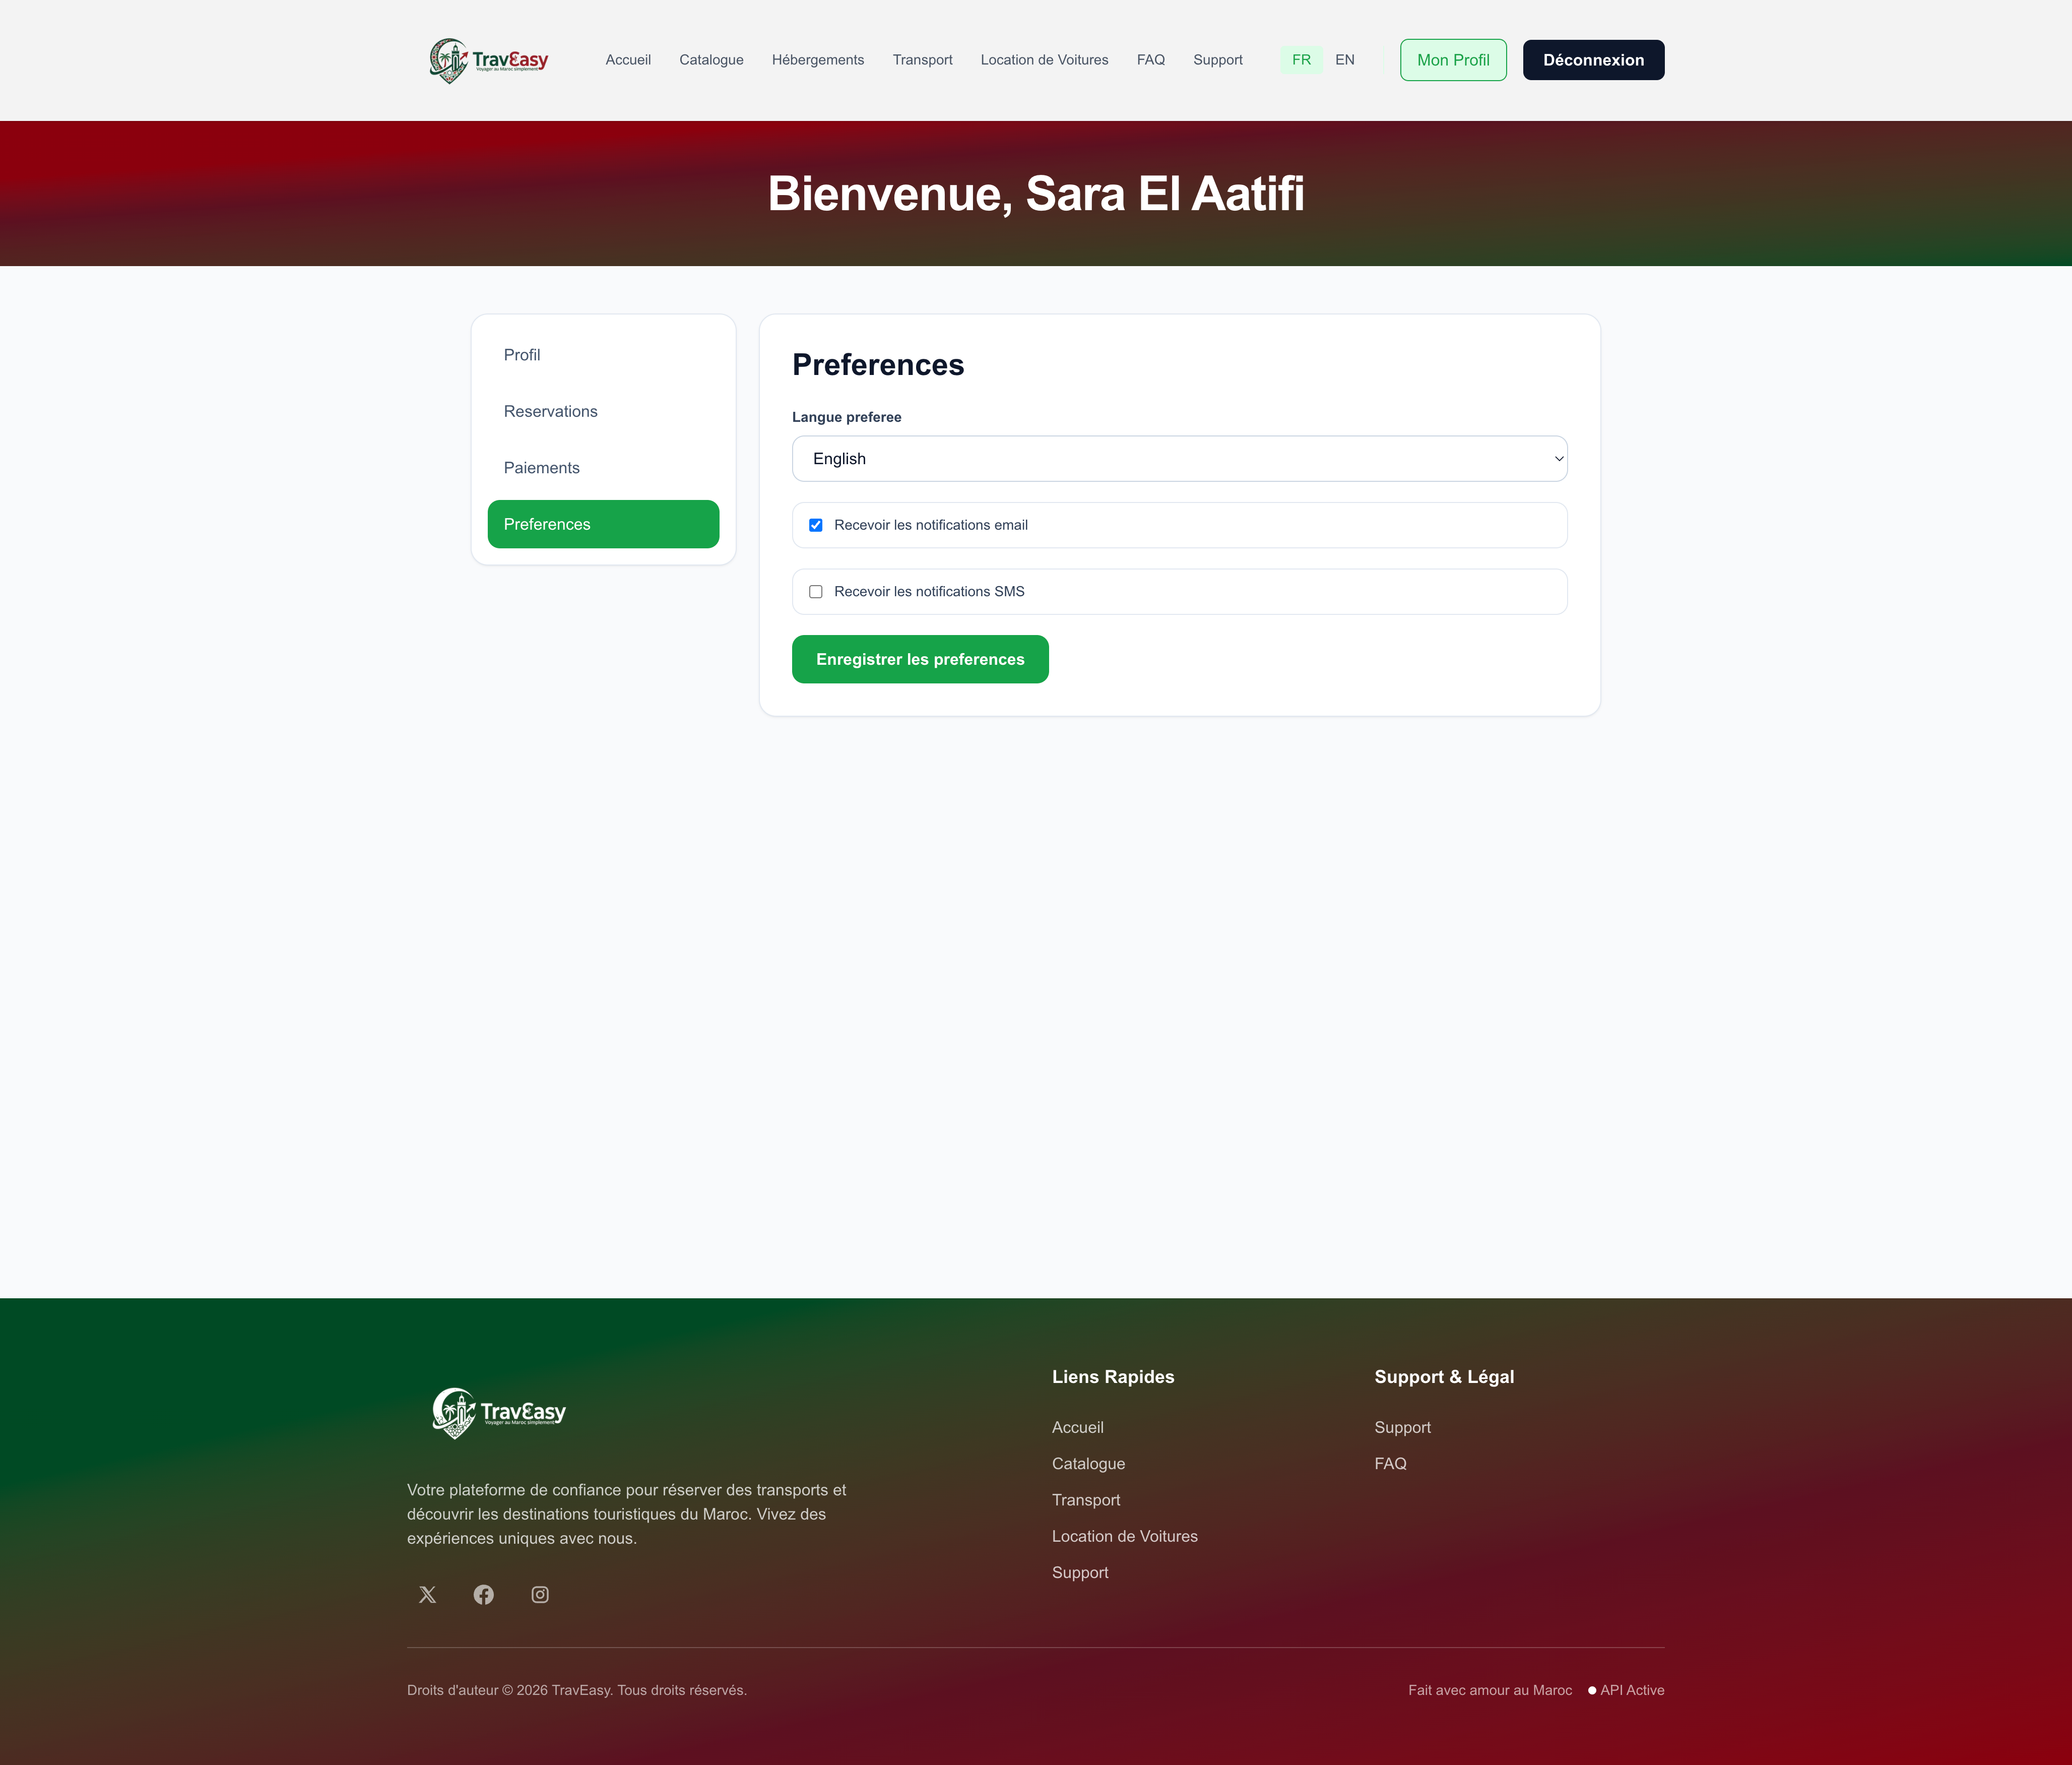
\includegraphics[width=\textwidth]{preference.png}
\caption{Onglet des préférences dans l’espace profil}
\label{fig:Onglet preferences profil}
\end{figure}

Cet onglet permet à l'utilisateur de personnaliser son expérience en gérant ses préférences, contribuant ainsi à une navigation plus adaptée à ses besoins et centres d'intérêt.

\end{spacing}



\subsection{Espace administrateur}
\vspace{0.5cm}
\begin{spacing}{1.5}
\justifying
L’espace administrateur constitue le module de gestion et de supervision de la plateforme. Il permet aux administrateurs de contrôler l’ensemble des données et des services afin d’assurer le bon fonctionnement du système. Ce module intègre des fonctionnalités de \textbf{gestion des utilisateurs}, permettant de consulter, modifier ou supprimer les comptes selon les besoins. Il offre également des outils de \textbf{gestion des lieux touristiques}, facilitant l’ajout, la mise à jour et la suppression des informations relatives aux destinations et activités proposées. En outre, l’administrateur peut assurer le suivi des opérations grâce à la \textbf{gestion des réservations}, qui permet de consulter et de contrôler les différentes demandes effectuées par les utilisateurs. Enfin, un tableau de bord dédié à la \textbf{consultation des statistiques} fournit une vue d’ensemble sur l’activité de la plateforme, notamment le nombre d’utilisateurs, de réservations et d’avis, contribuant ainsi à une meilleure prise de décision et à l’amélioration continue des services proposés.
%Ajouter des captures du tableau de bord administrateur.
\begin{figure}[H]
\centering
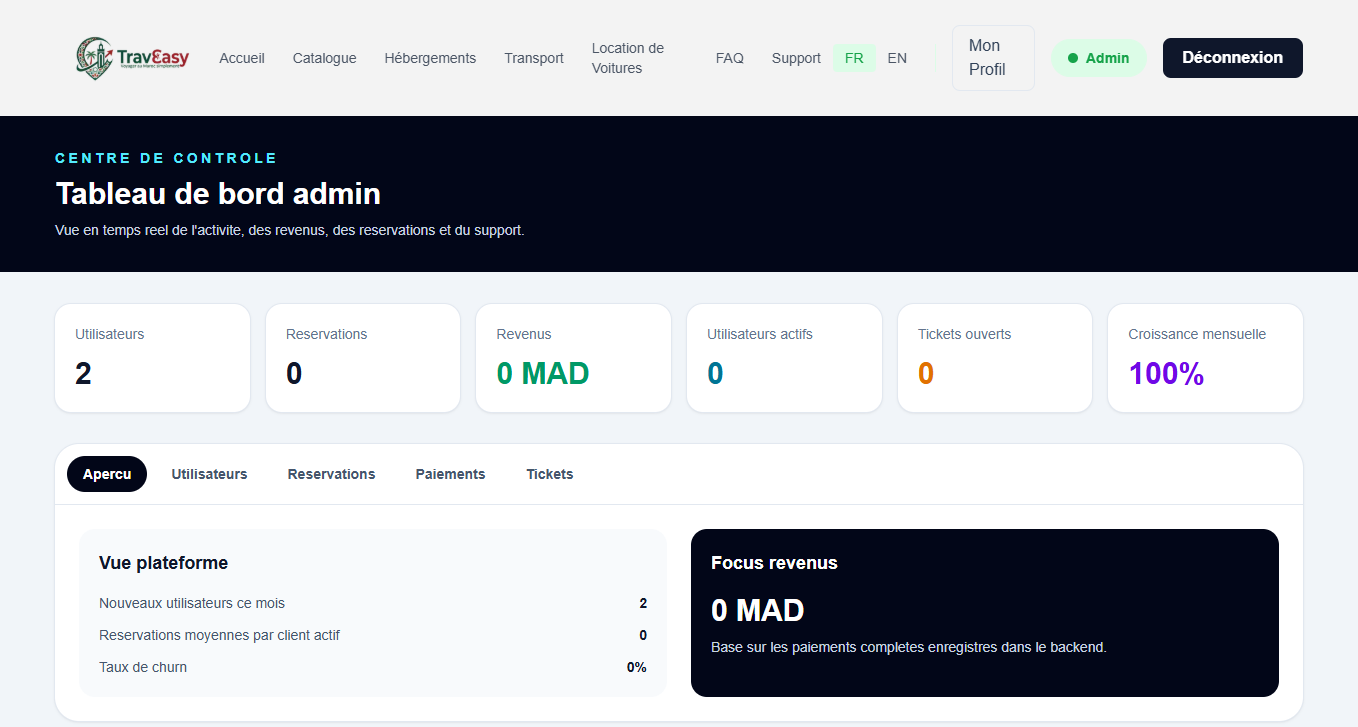
\includegraphics[width=\textwidth]{admin.png}
\caption{Tableau de bord administrateur}
\label{fig:Tableau de bord administrateur}
\end{figure}

Le tableau de bord administrateur offre une vue d'ensemble sur l'activité de la plateforme, incluant le nombre d'utilisateurs, de réservations et d'avis. Il centralise également les outils de gestion des utilisateurs, des lieux touristiques et des réservations, facilitant la supervision et la prise de décision.

\end{spacing}

\end{spacing}
\subsection{Module FAQ et support}
\vspace{0.5cm}
\begin{spacing}{1.5}
\justifying
Le module FAQ et support a été développé afin d'accompagner les utilisateurs tout au long de leur expérience sur la plateforme TravEasy. Il se compose de deux volets complémentaires : une \textbf{foire aux questions (FAQ)} et un \textbf{formulaire de contact et de support}.

La section FAQ regroupe les réponses aux interrogations les plus fréquentes des utilisateurs, couvrant des thématiques variées telles que la création de compte, la gestion des réservations, les modalités de paiement, et les conditions d'utilisation de la plateforme. Cette ressource permet aux utilisateurs de trouver des réponses rapidement et de manière autonome, sans nécessiter l'intervention du service d'assistance.

Le formulaire de contact permet quant à lui aux utilisateurs de soumettre des demandes d'assistance, de signaler des problèmes techniques ou d'envoyer des suggestions d'amélioration. Les messages sont transmis directement à l'équipe d'administration via un service d'envoi de courrier électronique sécurisé (SMTP), garantissant un traitement rapide et efficace des requêtes.

\begin{figure}[H]
\centering
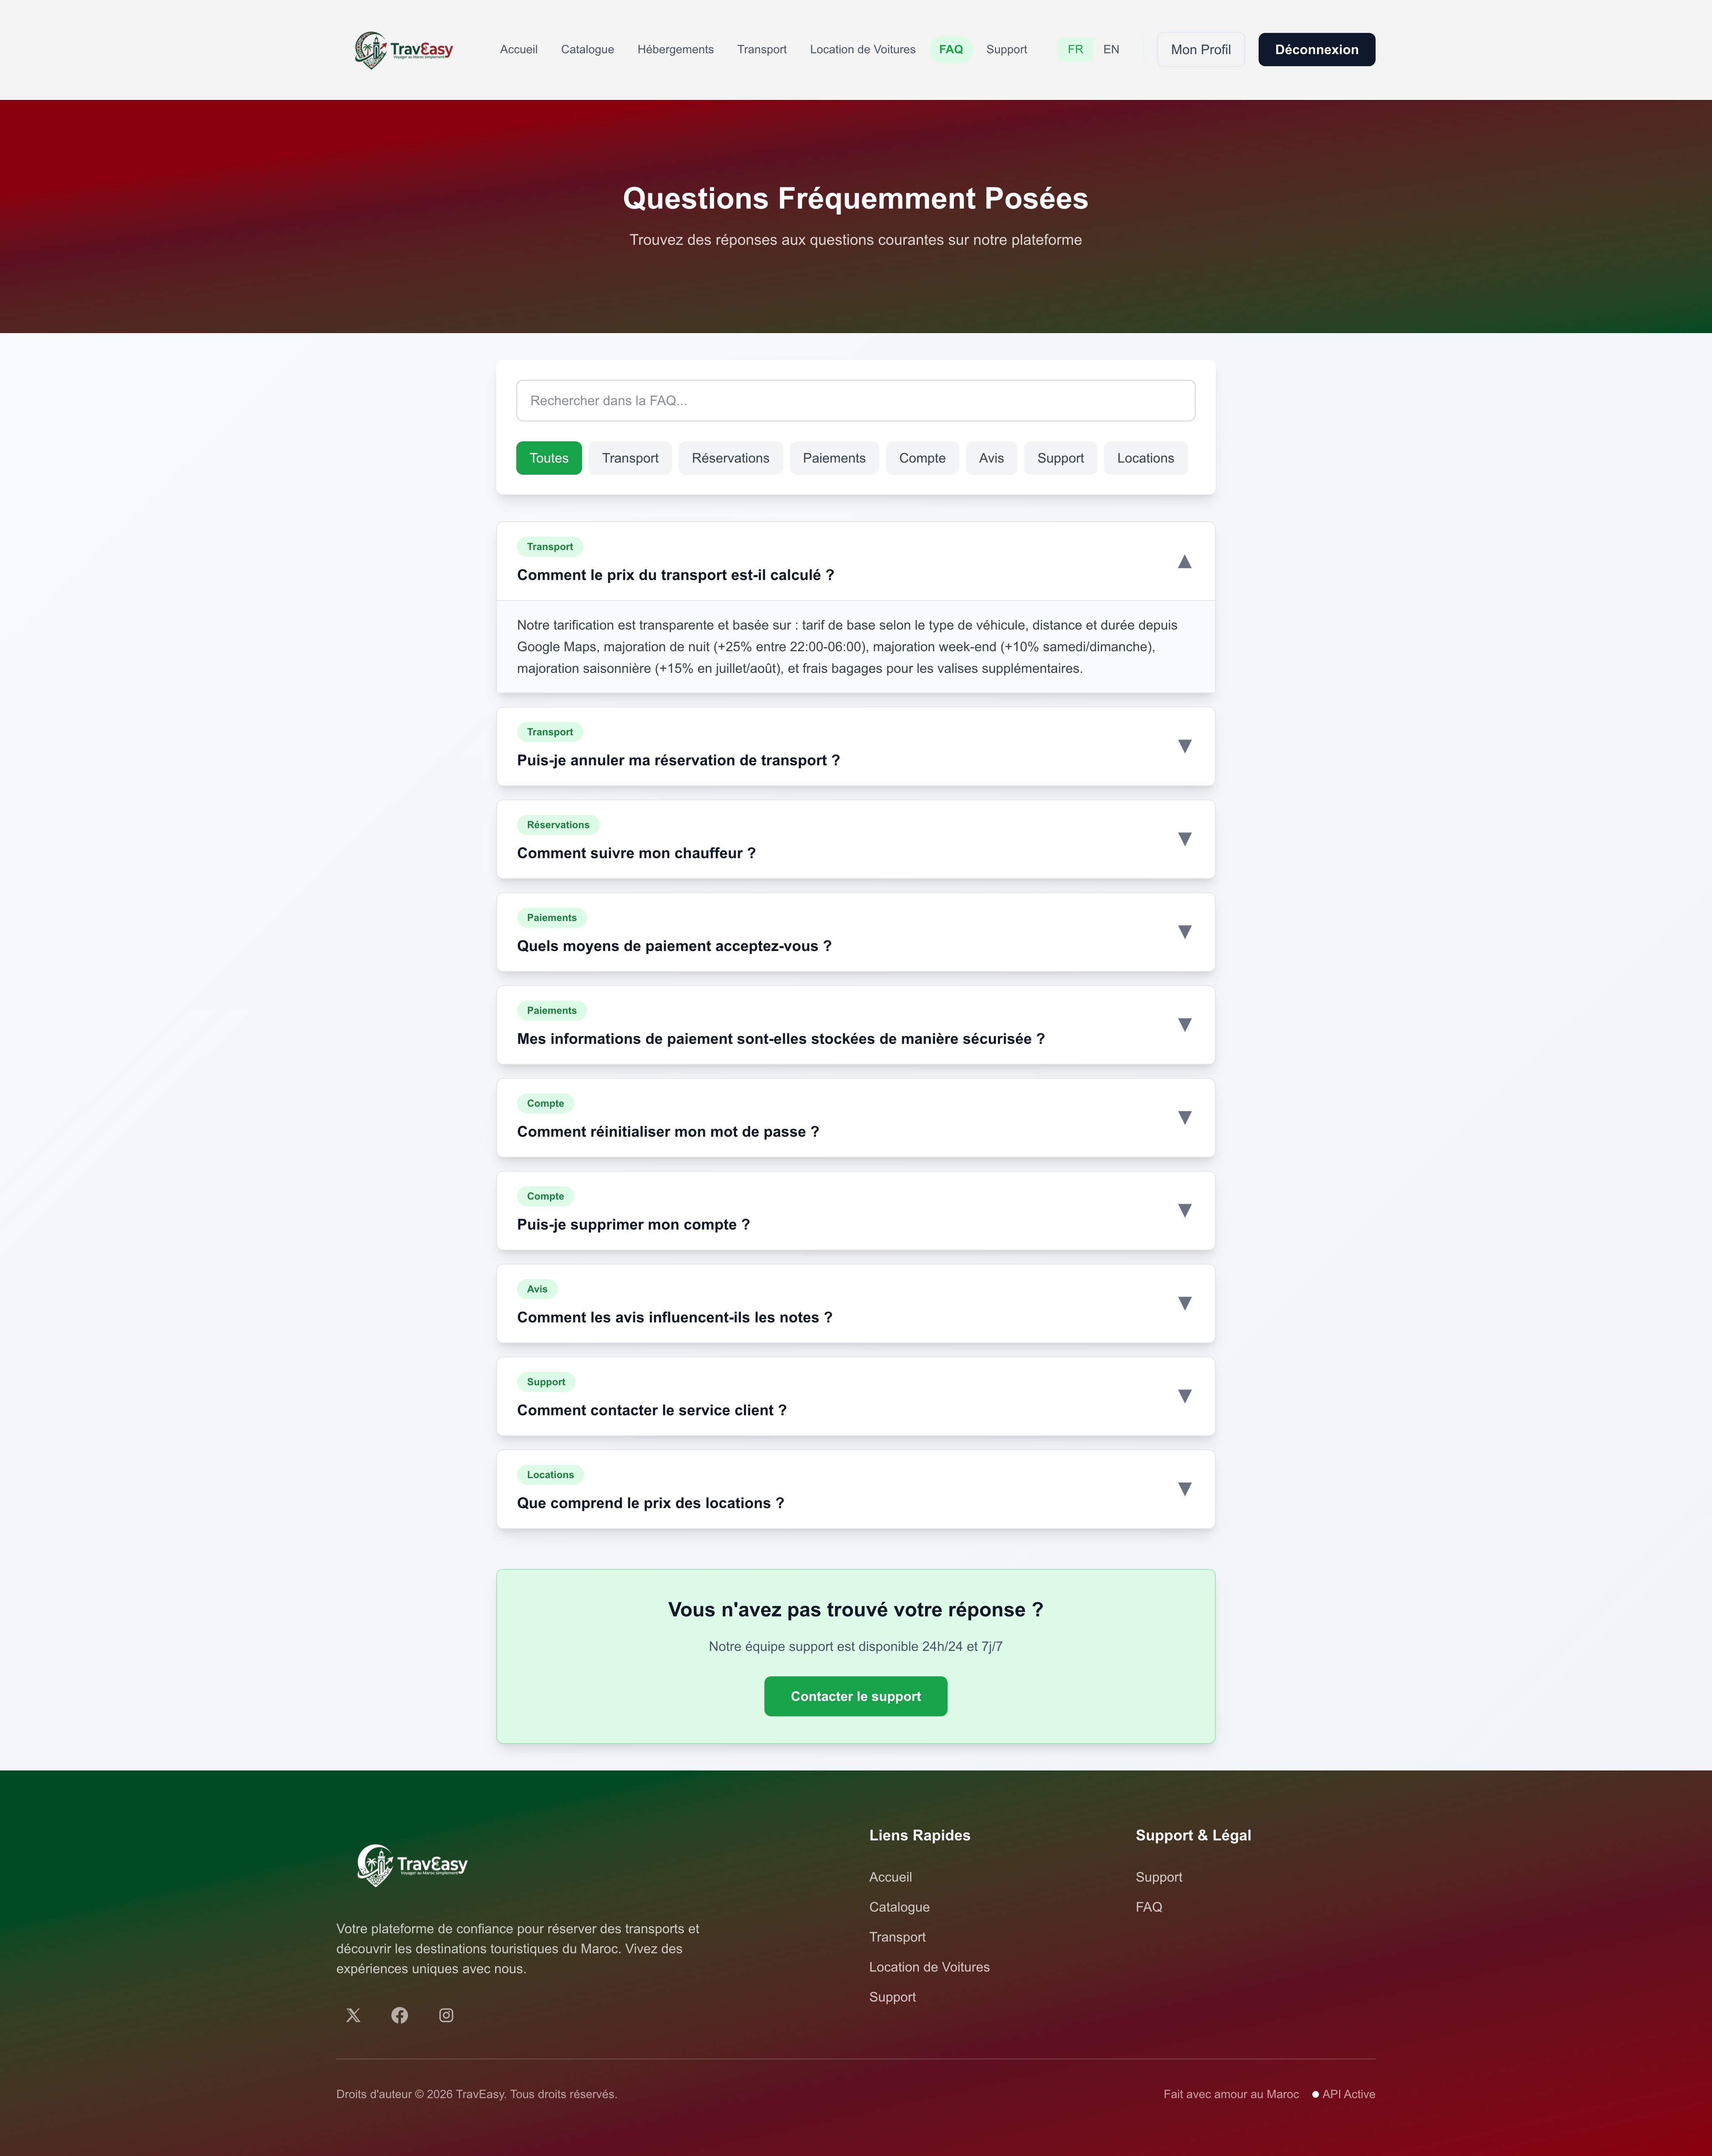
\includegraphics[width=0.85\textwidth]{faq.png}
\caption{Page FAQ de la plateforme TravEasy}
\label{fig:faq}
\end{figure}

La page FAQ regroupe les réponses aux questions les plus fréquentes des utilisateurs, couvrant des thématiques telles que la création de compte, la gestion des réservations, les modalités de paiement et les conditions d'utilisation, permettant une assistance autonome et rapide.

\begin{figure}[H]
\centering
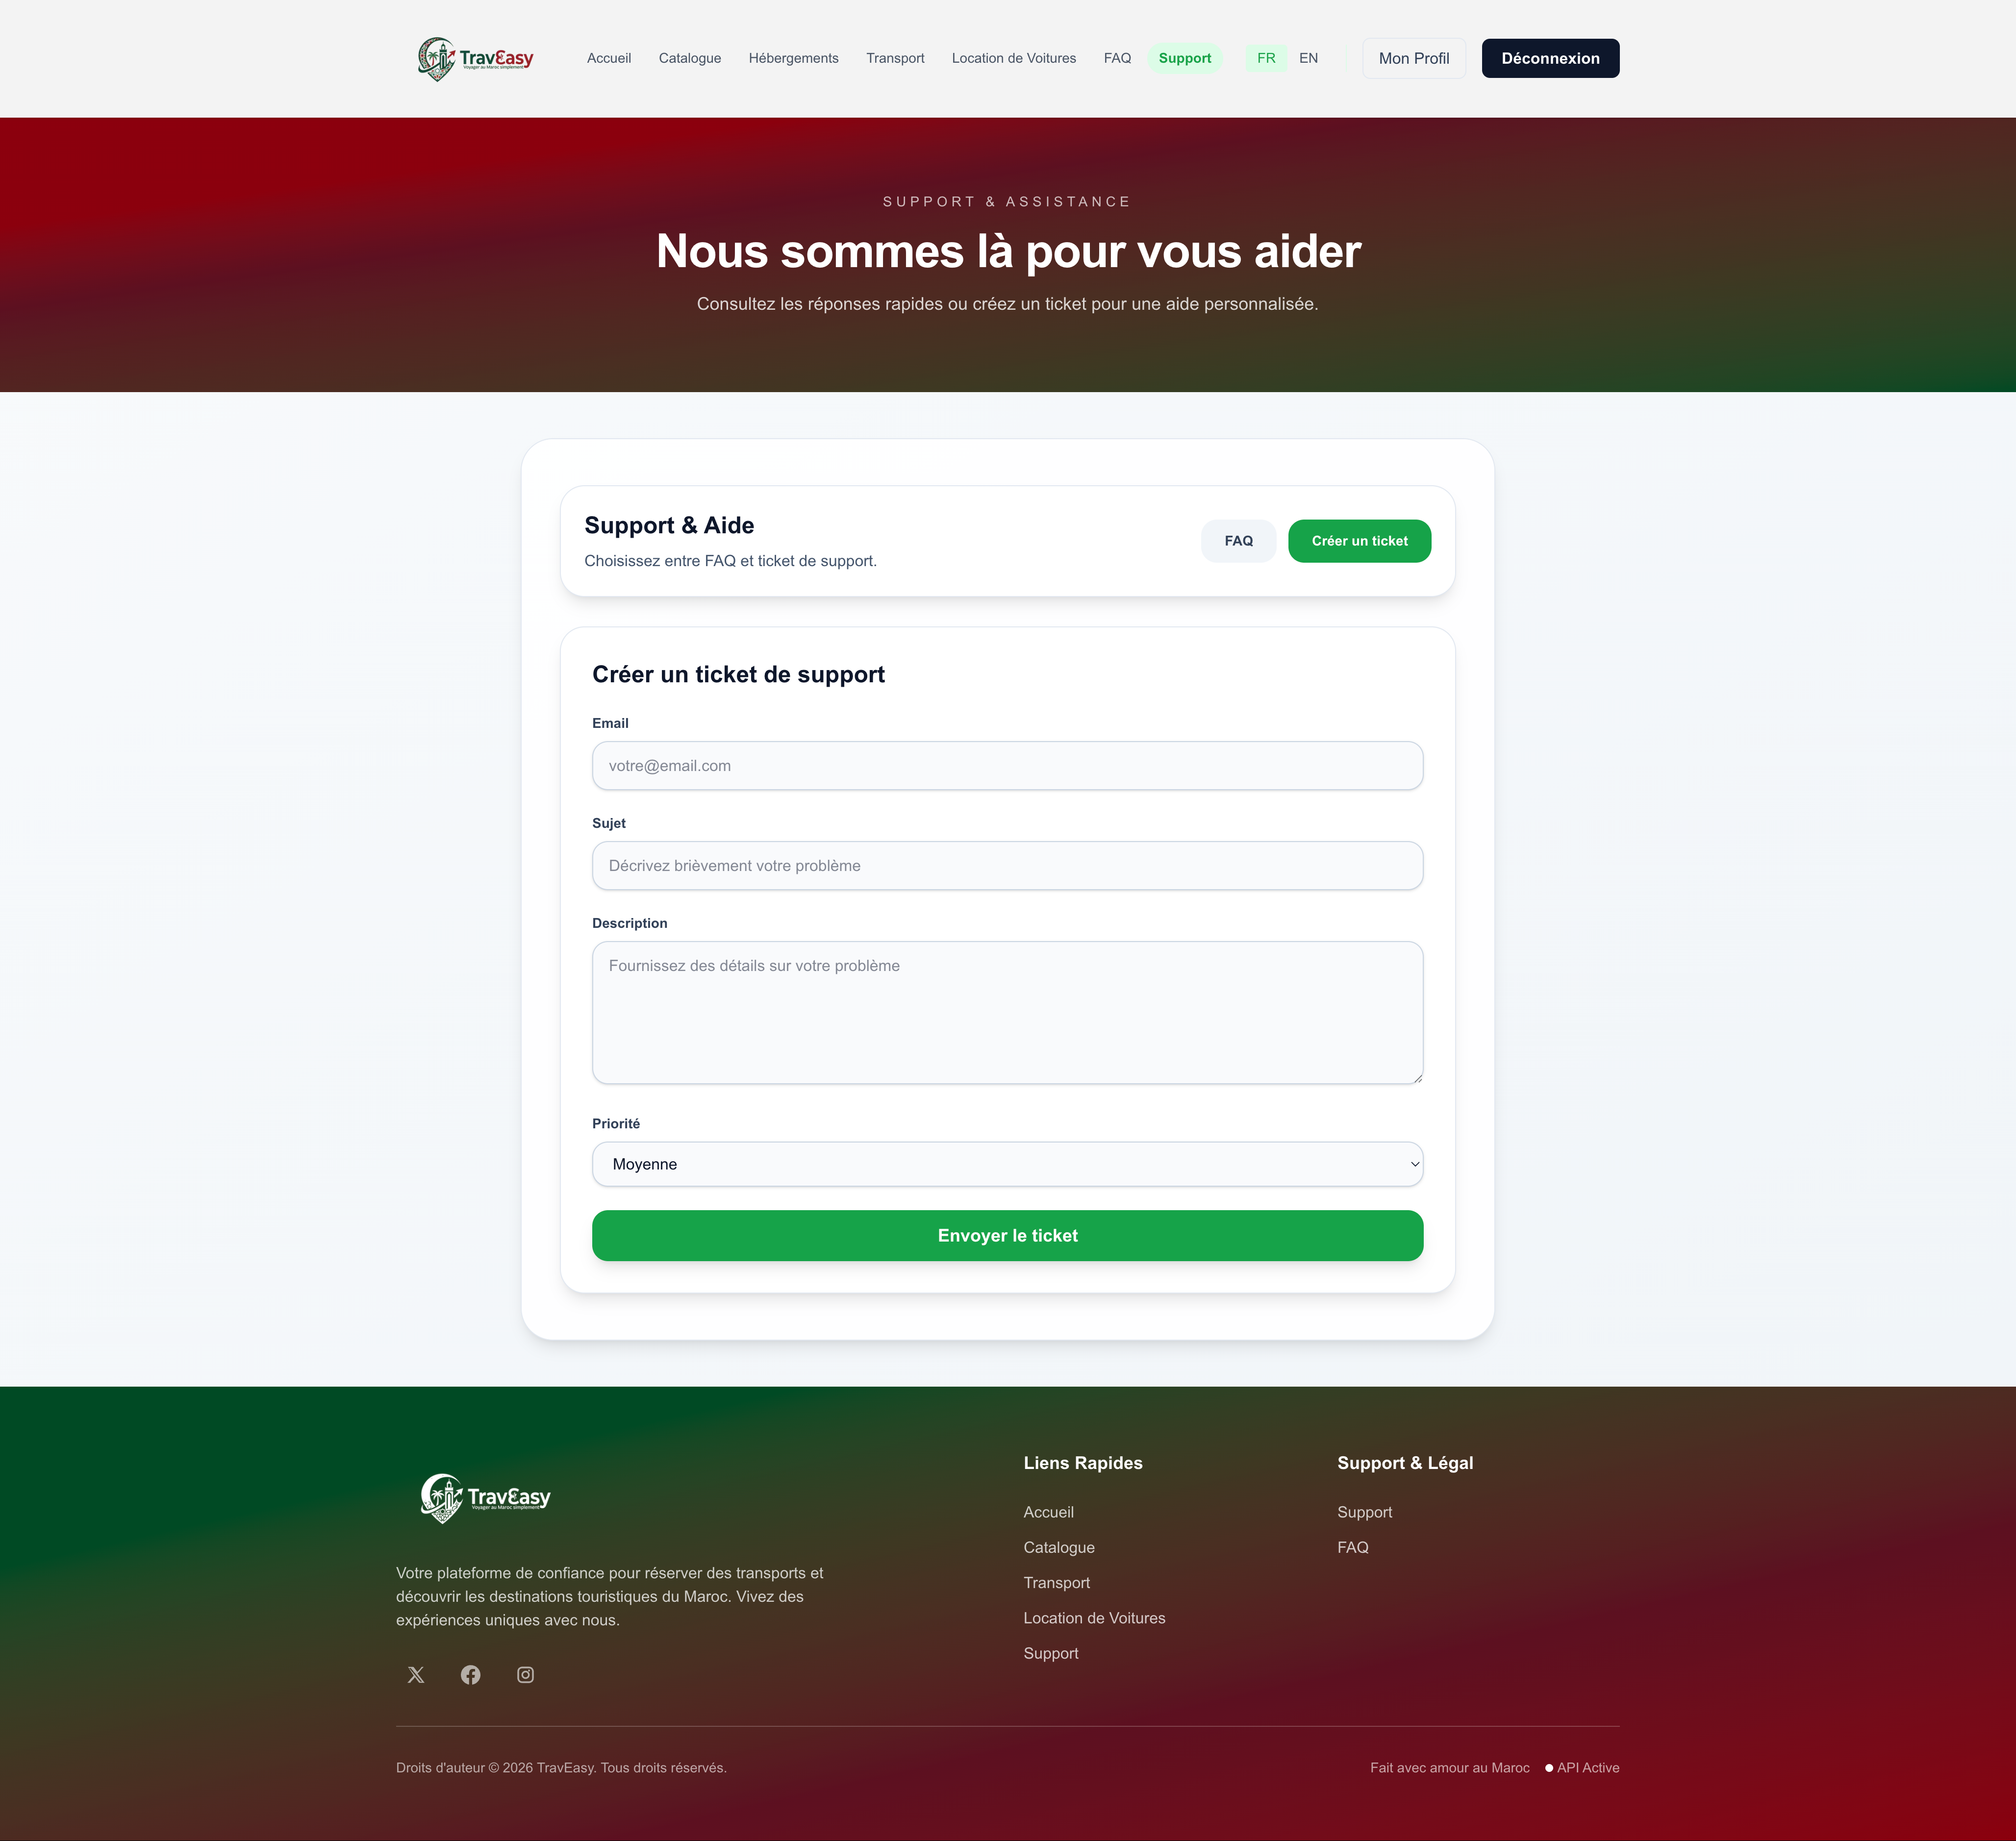
\includegraphics[width=0.85\textwidth]{support.png}
\caption{Formulaire de contact et de support}
\label{fig:support}
\end{figure}


Le formulaire de contact permet aux utilisateurs de soumettre des demandes d'assistance, de signaler des problèmes techniques ou d'envoyer des suggestions. Les messages sont transmis directement à l'équipe d'administration via un service SMTP sécurisé, garantissant un traitement rapide des requêtes.

\end{spacing}
\end{spacing}
\section{Implémentation des API REST}
\vspace{0.5cm}
\begin{spacing}{1.5}
\justifying
Afin d’assurer la communication entre le frontend et le backend, la plateforme repose sur une architecture basée sur des API REST. Ces interfaces permettent l’échange de données entre les différentes composantes du système à travers des requêtes HTTP standardisées. Plusieurs endpoints ont été développés pour répondre aux besoins fonctionnels de la plateforme.
\begin{itemize}
    \item \textbf{Authentification}
\end{itemize}
Les services d’authentification permettent la création de comptes utilisateurs et la gestion des connexions sécurisées.
\begin{StdTable}[H]{API d'Authentification}{tab:api_auth}{|X|X|X|}
\hline
\textbf{Méthode} & \textbf{Endpoint} & \textbf{Description} \\ \hline
POST & /api/auth/register & Inscription d’un nouvel utilisateur \\ \hline
POST & /api/auth/login & Authentification \\ \hline
\end{StdTable}

\begin{itemize}
    \item \textbf{Transport}
\end{itemize}
Les endpoints relatifs au transport permettent de calculer le coût d’un trajet et de gérer les réservations effectuées par les utilisateurs.
\begin{StdTable}[H]{API de Transport}{tab:api_transport}{|X|X|X|}
\hline
\textbf{Méthode} & \textbf{Endpoint} & \textbf{Description} \\ \hline
GET & /api/transport/price & Calcul du tarif d’un trajet \\ \hline
POST & /api/transport/book & Création d’une réservation de transport \\ \hline
\end{StdTable}
\begin{itemize}
    \item \textbf{Paiement}
\end{itemize}
Le module de paiement expose des services permettant d’effectuer des transactions sécurisées et de consulter l’historique des paiements.
\begin{StdTable}[H]{API de Paiement}{tab:api_paiement}{|X|X|X|}
\hline
\textbf{Méthode} & \textbf{Endpoint} & \textbf{Description} \\ \hline
POST & /api/payment & Traitement d’un paiement \\ \hline
GET & /api/payment/history & Consultation de l’historique des paiements \\ \hline
\end{StdTable}
\begin{itemize}
    \item \textbf{Lieux touristiques}
\end{itemize}
Ces endpoints permettent d’accéder aux informations relatives aux destinations et lieux touristiques disponibles sur la plateforme.
\begin{StdTable}[H]{API des Lieux Touristiques}{tab:api_places}{|X|X|X|}
\hline
\textbf{Méthode} & \textbf{Endpoint} & \textbf{Description} \\ \hline
GET & /api/places & Récupération de la liste des lieux touristiques \\ \hline
GET & /api/places/\{id\} & Consultation des détails d’un lieu touristique spécifique \\ \hline
\end{StdTable}
\textbf{CONCLUSION}
L’implémentation de ces API REST assure une séparation claire entre les couches de présentation et de traitement des données, favorisant ainsi la modularité, la maintenabilité et l’évolutivité de la plateforme.


\end{spacing}
\section{Sécurité de l’application}
\vspace{0.5cm}
\begin{spacing}{1.5}
\justifying
La sécurité constitue un aspect essentiel de la plateforme, notamment en raison de la gestion des données personnelles des utilisateurs, des réservations et des transactions financières. Afin de garantir la confidentialité, l’intégrité et la disponibilité des données, plusieurs mécanismes de sécurité ont été mis en œuvre.
\begin{itemize}
    \item \textbf{Authentification avec Firebase}
\end{itemize}
L’authentification des utilisateurs est assurée par \textbf{Firebase Authentication}. L’inscription et la connexion peuvent se faire soit via \textbf{e-mail/mot de passe}, soit via \textbf{SSO Google}. Après authentification, Firebase gère de manière sécurisée les jetons de session et l’identité des utilisateurs, ce qui permet de protéger l’accès aux ressources de la plateforme.
\begin{itemize}
    \item \textbf{Protection des mots de passe}
\end{itemize}
Les mots de passe des utilisateurs ne sont jamais stockés en clair. Pour les comptes créés avec e-mail/mot de passe, leur sécurisation est prise en charge par \textbf{Firebase Authentication}, qui applique des mécanismes de protection adaptés avant tout stockage. Cette approche renforce la sécurité des comptes utilisateurs en cas de compromission des données.
\begin{itemize}
    \item \textbf{Validation des entrées}
\end{itemize}
Toutes les données saisies par les utilisateurs font l’objet d’une validation côté client et côté serveur. Cette étape permet de vérifier la conformité des informations reçues et de prévenir les erreurs de saisie ainsi que certaines attaques exploitant des données malveillantes.
\begin{itemize}
    \item \textbf{Protection contre les injections SQL}
\end{itemize}
Afin de sécuriser les échanges avec la base de données, l’application utilise des requêtes paramétrées et des mécanismes de validation des données. Cette approche permet de limiter les risques d’\textbf{injection SQL}, l’une des attaques les plus courantes visant les applications web.
\begin{itemize}
    \item \textbf{Utilisation du protocole HTTPS}
\end{itemize}
Les communications entre les utilisateurs et le serveur sont protégées par le protocole \textbf{HTTPS}, qui assure le chiffrement des données échangées sur le réseau. Cette mesure garantit la confidentialité des informations sensibles et réduit les risques d’interception ou de modification des données lors de leur transmission.
\begin{itemize}
    \item \textbf{Sécurisation des paiements}
\end{itemize}
Les opérations de paiement sont réalisées à travers des plateformes spécialisées telles que \textbf{Stripe} et \textbf{PayPal}, reconnues pour leur haut niveau de sécurité. Ces services appliquent des mécanismes avancés de protection des transactions et assurent la conformité aux normes internationales de sécurité relatives aux paiements électroniques. Ainsi, les informations bancaires des utilisateurs ne sont jamais directement stockées ou traitées par la plateforme.

L’ensemble de ces mécanismes contribue à renforcer la sécurité globale de l’application, à protéger les données des utilisateurs et à garantir la fiabilité des services proposés par la plateforme.


\end{spacing}
\section{Conclusion}
\vspace{0.5cm}
\begin{spacing}{1.5}
\justifying
Ce chapitre a été consacré à la réalisation de la plateforme web touristique unifiée \textbf{TravEasy}. Nous y avons présenté l’environnement de développement adopté ainsi que les différentes technologies utilisées pour la conception et l’implémentation du système. Les principaux modules fonctionnels, notamment l’authentification, la recherche et la recommandation, la réservation de transport, le paiement, la gestion des avis ainsi que l’espace administrateur, ont également été détaillés. Enfin, l’implémentation des API REST et les mécanismes de sécurité mis en place ont permis de garantir la fiabilité, la performance et la protection des données au sein de la plateforme. L’ensemble de ces réalisations a abouti à une solution répondant aux objectifs fixés pour le projet et offrant une expérience utilisateur fluide et sécurisée. Le chapitre suivant sera consacré aux tests, à la validation et à l’évaluation de la plateforme développée.

\end{spacing}
\newpage
\chapter{ Tests et validation}
\newpage
\section{Introduction}
\vspace{0.5cm}
\begin{spacing}{1.5}
\justifying
À l’issue de la phase de réalisation, il est essentiel de procéder à une série de tests afin de vérifier la conformité et le bon fonctionnement de la plateforme web touristique unifiée \textbf{TravEasy}. Cette étape permet de s’assurer que les fonctionnalités implémentées répondent aux objectifs du projet et offrent un niveau satisfaisant de qualité, de performance et de sécurité. Elle vise également à identifier d’éventuelles anomalies et à valider la fiabilité du système dans différents scénarios d’utilisation.

Les tests effectués portent sur les principaux modules de la plateforme, notamment l’authentification des utilisateurs, la recherche et la consultation des lieux touristiques, la réservation de transport, le système de paiement ainsi que le module d’avis et de notation. Les résultats obtenus permettent d’évaluer le comportement de l’application et de confirmer son aptitude à répondre aux besoins des utilisateurs dans des conditions réelles d’exploitation.


\end{spacing}

\section{Stratégie de test}
\vspace{0.5cm}
\begin{spacing}{1.5}
\justifying
Afin de garantir la qualité et la fiabilité de la plateforme \textbf{TravEasy}, une stratégie de test a été mise en place tout au long du processus de validation. Cette démarche a permis de vérifier le bon fonctionnement des différentes fonctionnalités, d’assurer la cohérence des interactions entre les modules et d’évaluer la robustesse du système face à différents scénarios d’utilisation.

Les tests réalisés se répartissent en plusieurs catégories :

\begin{itemize}
    \item \textbf{Tests fonctionnels}
\end{itemize}
Les tests fonctionnels ont pour objectif de vérifier que chaque fonctionnalité de la plateforme répond correctement aux exigences prévues. Ils portent notamment sur l’authentification des utilisateurs, la recherche de lieux touristiques, la réservation de transport, le paiement en ligne ainsi que la gestion des avis et des notations.
\begin{itemize}
    \item \textbf{Tests d’intégration}
\end{itemize}
Les tests d’intégration visent à valider la communication et l’échange de données entre les différents modules de l’application. Ils permettent de s’assurer que les composants du système fonctionnent de manière cohérente lorsqu’ils sont utilisés conjointement.
\begin{itemize}
    \item \textbf{Tests de sécurité}
\end{itemize}
Les tests de sécurité ont été réalisés afin d’évaluer la protection des données et des accès utilisateurs. Ils concernent notamment l’authentification par SSO Google, email et mot de passe, la validation des entrées utilisateur et la protection contre les attaques courantes telles que les injections SQL.
\begin{itemize}
    \item \textbf{Tests de performance}
\end{itemize}
Les tests de performance permettent de mesurer la rapidité de traitement des requêtes ainsi que la réactivité globale de la plateforme. Ils ont pour objectif de vérifier que l’application offre une expérience utilisateur fluide même en présence de plusieurs utilisateurs ou de volumes importants de données.

L’ensemble de ces tests contribue à assurer la stabilité, la sécurité et la qualité globale de la plateforme avant sa mise en production.

\end{spacing}

\section{Tests fonctionnels}
\vspace{0.5cm}
\begin{spacing}{1.5}
\justifying
\subsection{Test du module d'inscription}
\vspace{0.5cm}
\begin{spacing}{1.5}
\justifying
\textbf{Objectif}

L’objectif de ce test est de vérifier qu’un nouvel utilisateur peut créer un compte sur la plateforme et que les mécanismes de validation des données fonctionnent correctement.

\textbf{Cas de test}
\begin{StdTable}[H]{Tests Fonctionnels - Inscription}{tab:test_inscription}{|X|X|X|X|}
\hline
\textbf{ID} & \textbf{Action} & \textbf{Résultat attendu} & \textbf{Résultat obtenu} \\ \hline
TF01 & Saisir des informations valides & Compte créé avec succès & Conforme \\ \hline
TF02 & Saisir une adresse e-mail déjà utilisée & Affichage d’un message d’erreur & Conforme \\ \hline
TF03 & Laisser le champ mot de passe vide & Refus de la création du compte & Conforme \\ \hline
\end{StdTable}


\textbf{Analyse des résultats}

Les tests réalisés sur le module d’inscription ont confirmé le bon fonctionnement du processus de création de compte. La plateforme accepte les informations valides et empêche l’enregistrement de données incorrectes ou incomplètes grâce aux mécanismes de validation mis en place. Les résultats obtenus sont conformes aux comportements attendus, ce qui permet de valider la fiabilité de cette fonctionnalité.

%Insérer ici une capture du formulaire d'inscription.

\end{spacing}

\subsection{Test du module de connexion}
\vspace{0.5cm}
\begin{spacing}{1.5}
\justifying
\textbf{Objectif}

L’objectif de ce test est de vérifier le bon fonctionnement du processus d’authentification des utilisateurs et de s’assurer que seuls les utilisateurs disposant d’identifiants valides peuvent accéder à la plateforme.

\textbf{Cas de test}
\begin{StdTable}[H]{Tests Fonctionnels - Connexion}{tab:test_connexion}{|X|X|X|X|}
\hline
\textbf{ID} & \textbf{Action} & \textbf{Résultat attendu} & \textbf{Résultat obtenu} \\ \hline
TF04 & Saisir une adresse e-mail et un mot de passe corrects & Connexion réussie & Conforme \\ \hline
TF05 & Saisir un mot de passe incorrect & Affichage d’un message d’erreur & Conforme \\ \hline
TF06 & Tenter une connexion avec un utilisateur inexistant & Accès refusé & Conforme \\ \hline
\end{StdTable}
%tableau 

\textbf{Analyse des résultats}

Les tests effectués sur le module de connexion ont permis de valider le mécanisme d’authentification mis en place. La plateforme autorise l’accès aux utilisateurs disposant d’identifiants valides et bloque les tentatives de connexion non autorisées. Les messages d’erreur sont correctement affichés lorsque les informations saisies sont incorrectes ou lorsqu’un compte n’existe pas. Les résultats obtenus sont conformes aux attentes, confirmant ainsi la fiabilité et la sécurité du processus d’authentification.


\end{spacing}

\subsection{Test du module de recherche touristique}
\vspace{0.5cm}
\begin{spacing}{1.5}
\justifying
\textbf{Objectif}

L’objectif de ce test est de valider le bon fonctionnement du moteur de recherche multicritère de la plateforme et de vérifier que les résultats affichés correspondent aux critères sélectionnés par l’utilisateur.

\textbf{Cas de test}
\begin{StdTable}[H]{Tests Fonctionnels - Recherche de lieux touristiques}{tab:test_recherche_lieux}{|X|X|X|X|}
\hline
\textbf{ID} & \textbf{Action} & \textbf{Résultat attendu} & \textbf{Résultat obtenu} \\ \hline
TF07 & Recherche par catégorie & Liste des lieux filtrée selon la catégorie choisie & Conforme \\ \hline
TF08 & Recherche par note & Résultats triés selon les notes attribuées & Conforme \\ \hline
TF09 & Recherche par prix & Résultats cohérents selon le critère de prix & Conforme \\ \hline
\end{StdTable}
%tableau 
\textbf{Analyse des résultats}

Les tests réalisés ont confirmé le bon fonctionnement du module de recherche touristique. Les recherches effectuées retournent correctement les lieux correspondant aux critères sélectionnés et les options de tri permettent d’afficher des résultats pertinents et cohérents. Les résultats obtenus sont conformes aux attentes, ce qui valide l’efficacité du moteur de recherche et améliore l’expérience de navigation des utilisateurs au sein de la plateforme.


\end{spacing}


\subsection{Test du module de réservation de transport}
\vspace{0.5cm}
\begin{spacing}{1.5}
\justifying
\textbf{Objectif}

L’objectif de ce test est de vérifier le bon fonctionnement du processus de réservation de transport, notamment le calcul automatique du tarif, l’enregistrement de la réservation et la génération de la facture associée.

\textbf{Cas de test}
\begin{StdTable}[H]{Tests Fonctionnels - Réservation de Transport}{tab:test_reservation_transport}{|X|X|X|X|}
\hline
\textbf{ID} & \textbf{Action} & \textbf{Résultat attendu} & \textbf{Résultat obtenu} \\ \hline
TF10 & Sélection d’un trajet & Affichage du prix calculé & Conforme \\ \hline
TF11 & Confirmation de la réservation & Réservation enregistrée avec succès & Conforme \\ \hline
TF12 & Génération de la facture & Facture créée au format PDF & Conforme \\ \hline
\end{StdTable}
%tableau

\textbf{Analyse des résultats}

Les tests effectués sur le module de réservation de transport ont confirmé le bon fonctionnement des différentes étapes du processus. Le système calcule correctement le tarif du trajet en appliquant les règles métier définies, notamment la prise en compte de la distance et des éventuelles majorations. L’enregistrement de la réservation est réalisé avec succès et une facture est automatiquement générée après validation de l’opération. Les résultats obtenus sont conformes aux attentes, ce qui permet de valider la fiabilité de ce module.


\end{spacing}

\subsection{Test du module d'hébergement}
\vspace{0.5cm}
\begin{spacing}{1.5}
\justifying
\textbf{Objectif}

L’objectif de ce test est de vérifier le bon fonctionnement du module d’hébergement, notamment les fonctionnalités de recherche, de filtrage, de pagination et d’accès aux informations détaillées des établissements touristiques.

\textbf{Cas de test}
\begin{StdTable}[H]{Tests Fonctionnels - Recherche d'Hébergements}{tab:test_hebergements}{|X|X|X|X|}
\hline
\textbf{ID} & \textbf{Cas de test} & \textbf{Résultat attendu} & \textbf{Résultat obtenu} \\ \hline
TH01 & Recherche par ville & Résultats filtrés selon la ville sélectionnée & Conforme \\ \hline
TH02 & Filtre par type d’hébergement & Affichage des hébergements correspondants & Conforme \\ \hline
TH03 & Filtre par nombre d’étoiles & Résultats corrects & Conforme \\ \hline
TH04 & Filtre par gamme de prix & Affichage correct des résultats & Conforme \\ \hline
TH05 & Pagination des résultats & Navigation correcte entre les pages & Conforme \\ \hline
TH06 & Bouton « Détails » & Redirection vers le site officiel de réservation & Conforme \\ \hline
\end{StdTable}
\textbf{Analyse des résultats}

Les tests réalisés ont permis de confirmer le bon fonctionnement de l’ensemble des fonctionnalités du module d’hébergement. Les recherches et les différents filtres appliqués retournent des résultats cohérents avec les critères sélectionnés par l’utilisateur. Le système de pagination facilite la navigation entre les résultats, tandis que la consultation des détails et les redirections vers les sites officiels des établissements s’effectuent correctement.

\end{spacing}
\subsection{Test du système de paiement}
\vspace{0.5cm}
\begin{spacing}{1.5}
\justifying
\textbf{Objectif}

L’objectif de ce test est de vérifier le bon fonctionnement du système de paiement en ligne, notamment la validation des transactions, la gestion des paiements refusés et la génération des reçus de paiement.

\textbf{Cas de test}
\begin{StdTable}[H]{Tests Fonctionnels - Paiement}{tab:test_paiement}{|X|X|X|X|}
\hline
\textbf{ID} & \textbf{Action} & \textbf{Résultat attendu} & \textbf{Résultat obtenu} \\ \hline
TF13 & Effectuer un paiement valide & Paiement accepté & Conforme \\ \hline
TF14 & Utiliser une carte refusée & Affichage d’un message d’erreur & Conforme \\ \hline
TF15 & Génération du reçu de paiement & Reçu disponible après validation du paiement & Conforme \\ \hline
\end{StdTable}
%tableau

\textbf{Analyse des résultats}

Les tests réalisés ont permis de valider le bon fonctionnement du système de paiement. Les transactions valides sont correctement traitées et confirmées, tandis que les paiements refusés génèrent des messages d’erreur appropriés. De plus, un reçu est automatiquement généré à l’issue de chaque transaction réussie. L’ensemble des opérations est enregistré de manière fiable, garantissant ainsi la traçabilité et la sécurité des transactions effectuées sur la plateforme.

\end{spacing}


\subsection{Test du système d'avis}
\vspace{0.5cm}
\begin{spacing}{1.5}
\justifying
\textbf{Objectif}

L’objectif de ce test est de vérifier le bon fonctionnement du module d’avis et de notation, notamment la publication des avis, l’attribution des notes et l’affichage des évaluations sur la plateforme.


\textbf{Cas de test}
\begin{StdTable}[H]{Tests Fonctionnels - Avis et Notations}{tab:test_avis_notations}{|X|X|X|X|}
\hline
\textbf{ID} & \textbf{Action} & \textbf{Résultat attendu} & \textbf{Résultat obtenu} \\ \hline
TF16 & Ajouter un avis & Avis enregistré avec succès & Conforme \\ \hline
TF17 & Attribuer une note & Recalcul automatique de la moyenne & Conforme \\ \hline
TF18 & Consulter les avis & Affichage correct des avis et des notes & Conforme \\ \hline
\end{StdTable}
%tableau 

\textbf{Analyse des résultats}

Les tests effectués ont permis de valider le bon fonctionnement du système d’avis et de notation. Les utilisateurs peuvent publier leurs avis sans difficulté, les notes attribuées sont correctement prises en compte dans le calcul de la moyenne et les informations sont affichées de manière cohérente sur la plateforme. Les résultats obtenus sont conformes aux attentes et confirment la fiabilité de ce module, qui contribue à améliorer la transparence et l’aide à la décision pour les utilisateurs.

\end{spacing}

\end{spacing}

\section{Tests d'intégration}
\vspace{0.5cm}
\begin{spacing}{1.5}
\justifying
\textbf{Objectif}

Les tests d’intégration ont pour objectif de vérifier la communication et l’échange de données entre les différents modules de la plateforme. Ils permettent de s’assurer que les composants développés fonctionnent correctement lorsqu’ils interagissent entre eux et que les informations sont transmises de manière cohérente tout au long des processus métier.

\textbf{Résultats des tests}
\begin{StdTable}[H]{Résultats des Tests d'Intégration}{tab:test_integration}{|X|X|}
\hline
\textbf{Modules testés} & \textbf{Résultat} \\ \hline
Authentification - Réservation & Conforme \\ \hline
Réservation - Paiement & Conforme \\ \hline
Paiement - Facturation & Conforme \\ \hline
Utilisateur - Avis & Conforme \\ \hline
Recherche - Base de données & Conforme \\ \hline
\end{StdTable}
%tableau
\textbf{Analyse des résultats}

Les tests réalisés ont confirmé le bon fonctionnement des interactions entre les différents modules de la plateforme. Les échanges de données s’effectuent correctement et les processus métier se déroulent sans interruption ni incohérence. Aucune anomalie majeure n’a été détectée lors des essais, ce qui démontre la bonne intégration des composants du système et contribue à garantir la stabilité et la fiabilité globales de l’application.

\end{spacing}


\section{Tests de sécurité}
\vspace{0.5cm}
\begin{spacing}{1.5}
\justifying
\textbf{Objectif}

Les tests de sécurité ont été réalisés afin de vérifier la robustesse de la plateforme face aux risques de sécurité les plus courants. Ils visent à garantir la protection des données des utilisateurs, la sécurisation des accès ainsi que la fiabilité des mécanismes d’authentification et d’autorisation.

\textbf{Vérifications réalisées}
\begin{StdTable}[H]{Résultats des Tests de Sécurité}{tab:test_securite}{|X|X|}
\hline
\textbf{Test} & \textbf{Résultat} \\ \hline
Authentification par SSO Google & Conforme \\ \hline
Authentification par email et mot de passe & Conforme \\ \hline
Hashage des mots de passe (bcrypt) & Conforme \\ \hline
Contrôle d’accès par rôle & Conforme \\ \hline
Validation des entrées utilisateur & Conforme \\ \hline
Protection contre les injections SQL & Conforme \\ \hline
\end{StdTable}
%tableau

\textbf{Analyse des résultats}

Les différents mécanismes de sécurité implémentés ont été testés avec succès. L’authentification basée sur Firebase assure un contrôle sécurisé des accès, 
 Les contrôles d’accès selon les rôles fonctionnent correctement et empêchent les utilisateurs non autorisés d’accéder aux ressources protégées. De plus, la validation des entrées et l’utilisation de requêtes sécurisées permettent de limiter efficacement les risques d’injection SQL et d’autres attaques courantes.


\end{spacing}

\section{Tests de performance}
\vspace{0.5cm}
\begin{spacing}{1.5}
\justifying
\textbf{Objectif}

Les tests de performance ont été réalisés afin d’évaluer la rapidité de réponse de la plateforme et de vérifier que les principales fonctionnalités offrent une expérience utilisateur fluide. Ces tests permettent de mesurer le temps nécessaire à l’exécution des opérations les plus importantes du système.

\textbf{Résultats des tests}
\begin{StdTable}[H]{Résultats des Tests de Performance}{tab:test_performance}{|X|X|}
\hline
\textbf{Fonctionnalité} & \textbf{Temps moyen} \\ \hline
Connexion & 0,8 s \\ \hline
Recherche touristique & 1,2 s \\ \hline
Réservation de transport & 1,4 s \\ \hline
Paiement & 1,8 s \\ \hline
\end{StdTable}
%tableau 

\textbf{Analyse des résultats}

Les résultats obtenus montrent que l’ensemble des fonctionnalités de la plateforme présente des temps de réponse satisfaisants. La connexion des utilisateurs s’effectue rapidement, tandis que les opérations plus complexes, telles que la réservation de transport et le traitement des paiements, restent exécutées dans des délais raisonnables. Les performances observées garantissent une navigation fluide et une utilisation confortable de la plateforme.



\end{spacing}

\section{Validation des objectifs du projet}
\vspace{0.5cm}
\begin{spacing}{1.5}
\justifying
\textbf{Objectif}

Cette étape vise à vérifier que l’ensemble des objectifs définis au début du projet a été atteint et que les fonctionnalités prévues ont été correctement implémentées au sein de la plateforme.

\textbf{Résultats de validation}
\begin{StdTable}[H]{Bilan des Objectifs du Projet}{tab:bilan_objectifs}{|X|X|}
\hline
\textbf{Objectif} & \textbf{Statut} \\ \hline
Gestion des utilisateurs & Atteint \\ \hline
Recherche multicritère & Atteint \\ \hline
Réservation de transport & Atteint \\ \hline
Paiement sécurisé & Atteint \\ \hline
Gestion des avis et notations & Atteint \\ \hline
Interface multilingue & Atteint \\ \hline
Tableau de bord administrateur & Atteint \\ \hline
\end{StdTable}
%tableau

\textbf{Analyse des résultats}

Les résultats obtenus montrent que l’ensemble des fonctionnalités prévues a été développé et validé avec succès. Les différents modules de la plateforme répondent aux besoins identifiés lors de l’analyse du projet et fonctionnent conformément aux attentes. Les tests réalisés ont permis de confirmer la stabilité, la sécurité et les performances de la solution mise en œuvre.


\end{spacing}

\section{Difficultés rencontrées et solutions apportées}
\vspace{0.5cm}
\begin{spacing}{1.5}
\justifying
Au cours du développement de la plateforme \textbf{TravEasy}, plusieurs difficultés techniques ont été rencontrées. Ces défis ont nécessité la mise en œuvre de solutions adaptées afin de garantir le bon fonctionnement et la fiabilité du système.
\begin{itemize}
    \item \textbf{Intégration de Google Maps}
\end{itemize}

\textbf{Problème :}

L’intégration des fonctionnalités de géolocalisation a présenté certaines difficultés, notamment la récupération des coordonnées géographiques des lieux ainsi que le calcul précis des distances entre différents points.

\textbf{Solution :}

Pour répondre à ce besoin, les services proposés par Google Maps API ont été utilisés. Cette solution a permis d’obtenir des données géographiques fiables et d’automatiser les calculs nécessaires à la réservation de transport et à l’affichage des informations de localisation.

\begin{itemize}
    \item \textbf{Gestion de l’authentification}
\end{itemize}

\textbf{Problème :}

La sécurisation des sessions utilisateurs et la protection des informations d’authentification représentaient un enjeu majeur pour la plateforme.

\textbf{Solution :}

Afin de garantir un niveau de sécurité élevé, un système d’authentification basé sur Firebase et SSO Google a été mis en place. De plus, les mots de passe sont protégés grâce à l’utilisation de bcrypt, qui assure leur hachage avant leur stockage dans la base de données.


\begin{itemize}
    \item \textbf{Gestion des paiements}
\end{itemize}

\textbf{Problème :}

La mise en œuvre d’un système de paiement sécurisé nécessitait une validation fiable des transactions et une protection efficace des données financières des utilisateurs.

\textbf{Solution :}

Cette problématique a été résolue par l’intégration de solutions de paiement reconnues telles que Stripe et PayPal. Les transactions sont vérifiées côté serveur avant leur validation définitive, garantissant ainsi la sécurité et l’intégrité des opérations financières.



\end{spacing}
%✅ 10 à 15 captures d'écran réelles de votre application
% Tableaux de cas de tests remplis avec résultats
%✅ Captures Postman des API testées
%✅ Captures de la base de données après insertion
%✅ Courbes ou graphiques de performance (si possible)
%✅ Tableau de validation des objectifs
%✅ Difficultés rencontrées et solutions apportées
%✅ Perspectives futures

\section{Conclusion}
\vspace{0.5cm}
\begin{spacing}{1.5}
\justifying
Ce chapitre a permis de valider la plateforme web touristique unifiée TravEasy à travers une série de tests fonctionnels, d’intégration, de sécurité et de performance. Les résultats obtenus ont confirmé le bon fonctionnement des différents modules, notamment l’authentification, la recherche touristique, la réservation de transport, le paiement en ligne, la gestion des avis ainsi que l’administration du système. Les mécanismes de sécurité mis en place ont démontré leur efficacité dans la protection des données et des accès utilisateurs, tandis que les tests de performance ont révélé des temps de réponse satisfaisants. Malgré certaines difficultés techniques rencontrées lors du développement, les solutions adoptées ont permis de garantir la fiabilité et la robustesse de la plateforme. L’ensemble des objectifs fixés au début du projet ayant été atteint, TravEasy constitue une solution fonctionnelle, sécurisée et adaptée aux besoins des utilisateurs dans le domaine du tourisme numérique.

\end{spacing}




\newpage
\section*{Conclusion Générale}
\addcontentsline{toc}{section}{Conclusion Générale}
\vspace{0.5cm}
\begin{spacing}{1.5}
\justifying
Au terme de ce projet de fin d’études, nous avons pu concevoir et développer TravEasy, une plateforme web touristique unifiée ayant pour objectif de faciliter l’accès aux principaux services touristiques au Maroc à travers une interface unique, moderne et intuitive.

Ce projet nous a permis d’appliquer les connaissances acquises tout au long de notre formation en Développement Informatique, notamment dans les domaines du développement web, de la modélisation UML, de la conception de bases de données, de la sécurité informatique et de la gestion de projets logiciels. L’étude préalable réalisée nous a permis d’identifier les limites des solutions existantes ainsi que les besoins des utilisateurs, servant ainsi de base à la conception d’une solution adaptée au contexte touristique marocain.

La plateforme développée intègre plusieurs fonctionnalités essentielles, notamment la consultation des destinations touristiques, la recherche et le filtrage d’hébergements, la réservation de transports aéroportuaires, la gestion des avis et des notations ainsi qu’une interface bilingue français–anglais destinée à répondre aux attentes d’une clientèle nationale et internationale. L’utilisation de technologies modernes telles que React.js, Node.js, Express.js et MySQL a permis de développer une application performante, évolutive et sécurisée.

Les différentes phases de tests réalisées ont permis de valider le bon fonctionnement des modules développés et de vérifier la conformité de la plateforme aux objectifs définis lors de la phase d’analyse. Les résultats obtenus démontrent que TravEasy constitue une solution pertinente permettant d’améliorer l’expérience utilisateur tout en contribuant à la valorisation de l’offre touristique marocaine à travers les technologies numériques.

Au-delà des objectifs atteints, plusieurs perspectives d’amélioration peuvent être envisagées pour enrichir davantage la plateforme. Parmi celles-ci figurent l’intégration d’un système de réservation directe des hébergements, le développement d’une application mobile, l’ajout de nouvelles langues ainsi que l’intégration de mécanismes de recommandation intelligente permettant de personnaliser davantage l’expérience utilisateur.

Enfin, cette expérience a représenté une opportunité enrichissante tant sur le plan technique que personnel. Elle nous a permis de développer nos compétences en analyse, conception et développement d’applications web tout en renforçant notre capacité à travailler en équipe et à mener à bien un projet informatique complet.

\end{spacing}


\end{document}